%\documentclass[12pt]{amsart}
%\documentclass[12pt]{article}
\documentclass[a4paper,12pt]{report}
\usepackage{titlesec}
%\defbibheading{bibliography}[\refname]{\section*{#1}}
%\titleformat{\chapter}
%\special{papersize=210mm,297mm}
%\setlength{\oddsidemargin}{2cm}
%\setlength{\evensidemargin}{3cm}
%\setlength{\textwidth}{2in}
%\setlength{\textheight}{3in}
%\setlength{\topmargin}{3cm}
%\setlength{\headheight}{0in}
%\setlength{\headsep}{0in}
%\pagestyle{empty}
\usepackage[style=abnt, language=brazil, natbib = true]{biblatex} 
\addbibresource{mypapers.bib}
\usepackage{etoolbox}
\AtBeginEnvironment{table}{\singlespacing}
\usepackage{parskip}
\setlength{\parindent}{1.25cm}
\setlength{\parskip}{0em}
\renewcommand{\baselinestretch}{1.5}
\pagestyle{myheadings}
\markright{}
\usepackage[lmargin=3.0cm,rmargin=2.0cm,tmargin=3.0cm,bmargin=2.0cm]{geometry}
%\usepackage{geometry}
%\geometry{letterpaper}
%\geometry{landscape}
%\usepackage[parfill]{parskip}
%\usepackage{ucs}
\usepackage[utf8]{inputenc}
\usepackage{indentfirst}
\usepackage[portuguese,english]{babel}
%\usepackage{times}
\interfootnotelinepenalty=10000
\usepackage[T1]{fontenc}
\usepackage{graphicx}
\usepackage{amsmath}
\usepackage{boxedminipage}
\usepackage{ragged2e}
\usepackage{leqno}
\usepackage{array}
\usepackage{amssymb, latexsym}
\usepackage{epstopdf}
\usepackage{subfigure}
\usepackage{pdfpages}
%\usepackage[colorlinks=true,allcolors=blue]{hyperref} % simplify
\usepackage[colorlinks=true,allcolors=black]{hyperref} % simplify
%\usepackage[round]{natbib}
\usepackage{threeparttable}
\usepackage{tabularx}
\usepackage{graphicx}
\usepackage{float}
\usepackage{rotating}
\usepackage{booktabs}
\usepackage{caption}
\usepackage[toc,page]{appendix}
\newtheorem{theorem}{Theorem}
\newtheorem{lemma}{Lemma}
\newtheorem{definition}{Definition}
\newtheorem{notation}{Notation}
\newtheorem{assump}{Assumption}
\newtheorem{proposition}{Proposition}
\newtheorem{corollary}{Corollary}[theorem]
\DeclareGraphicsRule{.tif}{png}{.png}{`convert #1 `dirname #1`/`basename #1 .tif`.png}
\DeclareMathOperator{\diag}{diag}
\DeclareMathOperator{\Ima}{Im}
\setlength{\parindent}{18.75pt}
\hypersetup{
	pdftitle={TITLE},
	pdfauthor={AUTHOR},
	pdfsubject={SUBJECT},
	pdfkeywords={KEYWORD} {KEYWORD} {KEYWORD},
	colorlinks=true,
	linkcolor=black,
	citecolor=black,
	filecolor=black,
	urlcolor=black
}
\usepackage{setspace}
%\onehalfspacing


\usepackage[labelfont=bf]{caption} %% for the figure and Tables Caption%%
%\usepackage[textfont=bf]{caption}
\usepackage{standalone}

\makeatletter
\renewcommand*\@makechapterhead[1]{%
	%\vspace*{50\p@}%
	{\parindent \z@ \raggedright \normalfont
		\ifnum \c@secnumdepth >\m@ne
		\huge\bfseries \thechapter \space %\@chapapp\space \thechapter
		%   \par\nobreak
		%  \vskip 20\p@
		\fi
		\interlinepenalty\@M
		\Huge \bfseries #1\par\nobreak
		\vskip 40\p@
}}
\renewcommand*\@makeschapterhead[1]{%
	%\vspace*{50\p@}%
	{\parindent \z@ \raggedright
		\normalfont
		\interlinepenalty\@M
		\Huge \bfseries  #1\par\nobreak
		\vskip 40\p@
}}
\makeatother

\makeatletter
\renewcommand\l@section{\@dottedtocline{1}{0em}{3em}}
\renewcommand\l@subsection{\@dottedtocline{2}{0em}{3em}}
\makeatother
% Some useful commands %%%%%%%%%%

\newcommand{\chapfnt}{\fontsize{12}{19}}
\newcommand{\secfnt}{\fontsize{12}{17}}
\newcommand{\ssecfnt}{\fontsize{12}{14}}
\titleformat{\chapter}[display]
{\normalfont\chapfnt\bfseries}{\chaptertitlename\ \thechapter}{12pt}{\chapfnt}

\titleformat{\section}
{\normalfont\secfnt\bfseries}{\thesection}{1em}{}

\titleformat{\subsection}
{\normalfont\ssecfnt\bfseries}{\thesubsection}{1em}{}

\titlespacing*{\chapter} {0pt}{50pt}{40pt}
\titlespacing*{\section} {0pt}{3.5ex plus 1ex minus .2ex}{2.3ex plus .2ex}
\titlespacing*{\subsection} {0pt}{3.25ex plus 1ex minus .2ex}{1.5ex plus .2ex}



\newcommand\Kh{K\left( \frac{X_i-x}{h_n} \right)}
\newcommand\Kpsi{K\left( \frac{\psi-x}{h_n} \right)}
\newcommand\Xh{\left( \frac{X_i-x}{h_n} \right)}
\newcommand\Xpsi{\left( \frac{\psi-x}{h_n} \right)}
\newcommand\kh{K\left( \frac{X_i-x}{h_n} \right)}
\newcommand\kg{K\left( \frac{X_i-x}{g_n} \right)}
\newcommand\kpsi{K\left( \frac{\psi-x}{h_n} \right)}
\newcommand\xh{\left( \frac{X_i-x}{h_n} \right)}
\newcommand\xpsi{\left( \frac{\psi-x}{h_n} \right)}
\newcommand\lla{L^{(2)}(\lambda_i(X_i-x),\hat{\theta}(x))}
\newcommand\hl{\sigma^{2(2)}(\lambda_{i}^{'}(X_i-x) + x)}
\newcommand\hp{\sigma^{2(1)}(\lambda_{i}^{'}(X_i-x) + x)}
\newcommand\oh{\hat{\theta}(x)}
\newcommand\ohone{\hat{\theta}_1(x)}
\newcommand\ohtwo{\hat{\theta}_2(x)}
\newcommand\ohtt{\hat{\theta}_{2}(x)^{2}}
\newcommand\ott{{\theta}_{2}(x)^{2}}
\newcommand\Rx{R_i(X_i - x)^2}
\newcommand\Rc{\mathbb{R}}

%%%%%%%%%%%%%%%%%%%%%%%

\begin{document}
	
	\defbibheading{bibliography}[\refname]{\section*{#1}}
	
	\begin{titlepage}
		\setlength{\baselineskip}{24pt}
		\centering
		%\begin{center}
		
		\large \bf{
			UNIVERSIDADE FEDERAL DO RIO GRANDE DO SUL \\
			FACULDADE DE CIÊNCIAS ECONÔMICAS \\
			PROGRAMA DE PÓS-GRADUAÇÃO EM ECONOMIA \\ [3cm]
			
			FERNANDO A. BOEIRA SABINO DA SILVA \\ [3cm]
			
			
			{ENSAIOS EM CÓPULAS E FINANÇAS EMPÍRICAS} \\
			
			\vfill
			Porto Alegre \\
			2017}
		
		%\end{center}
		
		
		
	\end{titlepage}

%\includegraphics[angle=0,origin=c,page=1,width=\textwidth]{ficha_catalografica.pdf}

\includepdf{ficha_catalografica.pdf}

	\begin{titlepage}
		\setlength{\baselineskip}{24pt}
		\centering
		%\begin{center}
		\large {
			
			\textbf{FERNANDO A. BOEIRA SABINO DA SILVA} \\ [6cm]
			
			
			\textbf{ENSAIOS EM CÓPULAS E FINANÇAS EMPÍRICAS} \\ [4cm]
			
			
			
			%\begin{flushright}
			\hfill
			\hspace{.45\textwidth}
			\begin{minipage}{.5\textwidth}
				\singlespacing
				Tese submetida ao Programa de Pós-Graduação em Economia da Faculdade de Ciências Econômicas da UFRGS, como quesito parcial para obtenção do título de Doutor em Economia, com ênfase em Economia Aplicada.  \\ [1cm]
				Orientador: Prof. Dr. Flávio A. Ziegelmann \\
			\end{minipage}
			
			%\end{flushright}
			
			
			\vfill
			\bf{
				Porto Alegre \\
				2017}
		}
	\end{titlepage}
	
	
	%%%%%%%%%%%%%%%%%%%%%%%%%%%%%%
	%%% Folha biblioteca %%%%%%%%%%%%%%%%%%
	%%%%%%%%%%%%%%%%%%%%%%%%%%%%%%
	%\includepdf{cip.pdf}
	% comando para incluir a folha fornecida pela biblioteca.
	%%%%%%%%%%%%%%%%%%%%%%%%%%%%%%
	%folha de aprovacao
	
	
	\begin{titlepage}
		\singlespacing
		\setlength{\baselineskip}{24pt}
		\centering
		%\begin{center}
		\large {
			
			\textbf{FERNANDO A. BOEIRA SABINO DA SILVA} \\ [2cm]
			
			
			\textbf{ENSAIOS EM CÓPULAS E FINANÇAS EMPÍRICAS} \\ [1.5cm]
			
			
			
			%\begin{flushright}
			\hfill
			\hspace{.45\textwidth}
			\begin{minipage}{.5\textwidth}
				\singlespacing
				Tese submetida ao Programa de Pós-Graduação em Economia da Faculdade de Ciências Econômicas da UFRGS, como quesito parcial para obtenção do
				título de Doutor em Economia, com ênfase em Economia Aplicada.  \\ [1cm]
				%Orientador: Prof. Dr. Flávio A. Ziegelmann \\ [1cm]
			\end{minipage}
			
			%\end{flushright}
			
			\begin{flushleft}
			\noindent
			Aprovada em: Porto Alegre, 25 de abril de 2017.\\
			\vspace{1.5cm}
			
			\noindent
			BANCA EXAMINADORA:\\
			%
			
			\vspace{4pt}
			\noindent
			\rule{\textwidth}{1pt}
			Prof. Dr. Flávio Augusto Ziegelmann -- Orientador\\
			UFRGS\\
			
			\vspace{4pt}
			\noindent
			\rule{\textwidth}{1pt}
			Prof. Dr. André Alves Portela Santos\\
			UFSC\\
			
			\vspace{4pt}
			\noindent
			\rule{\textwidth}{1pt}
			Prof. Dr. Guilherme Valle Moura\\
			UFSC\\
			
			\vspace{4pt}
			\noindent
			\rule{\textwidth}{1pt}
			Prof. Dr. Tiago Pascoal Filomena\\
			UFRGS\\
			
			\end{flushleft}
			
}		
	\end{titlepage}
	
	
	\begin{titlepage}
		
		\setlength{\topmargin}{22cm}
		\hfill{Para os meus pais (in memorian).}
	\end{titlepage}
	
	
	\begin{center}
		%\Large \bf
		\section*{\centerline{AGRADECIMENTOS}}
	\end{center}

 		\vspace{0.3cm}
 
		Sou muito grato a todos que me ajudaram nesta caminhada, em especial aos meus pais, irmãos, Cristina e a sua família. 
		
		\vspace{0.3cm}
		
		O amor é o alimento da vida. Cristina me ajudou a trilhar por caminhos com um número muito menor de espinhos, usando muito tempo para me deixar mais seguro de que estava indo na direção correta e sendo exemplo de disciplina.
		
		\vspace{0.3cm}
		
			Ao prof. Flávio pelos ensinamentos, incluindo os exemplos de justiça, correção e sensibilidade.
			
		\vspace{0.3cm}
			
			Aos membros da banca examinadora, pelo tempo dispensado na leitura deste trabalho e pelos comentários e críticas.
			
		\vspace{0.3cm}
			
		Aos meus colegas, em especial Hudson e Gabrielito.
		
		\vspace{0.3cm}
		
		A Tainan por toda a ajuda na editoração final da tese.
		
		\vspace{0.3cm}
		
		Aos professores e técnicos administrativos do PPGE pela dedicação e por todo o apoio.
		
		\vspace{0.3cm}
		
		A todos aqueles que não tenham sido citados aqui, mas que de algum modo colaboraram para a realização deste trabalho.
		
		\vspace{0.3cm}
		
		Por fim, que eu possa aplicar o que recebi para o propósito do bem, desviando de mim os maus pensamentos como o orgulho. 



		%\addcontentsline{toc}{section}{\bf{Resumo}}
		
	%\end{center}
	\thispagestyle{empty}
	
	\setlength{\baselineskip}{24pt}
	
	
	\clearpage
	
	
	%\pagenumbering{roman}
	%\setcounter{page}{1}
	
	%\begin{center}
		%\Large \bf
		\section*{\centerline{RESUMO}}
		%\addcontentsline{toc}{section}{\bf{Resumo}}
	%\end{center}
	\thispagestyle{empty}
	
	\begin{refsection}
	
	\setlength{\baselineskip}{12pt}
	\noindent Nesta tese discutimos abordagens que utilizam cópulas para descrever dependências entre instrumentos financeiros e avaliamos a performance destes métodos. Muitas crises financeiras aconteceram desde o final da década de 90, incluindo a crise asiática (1997), a crise da dívida da Rússia (1998), a crise da bolha da internet (2000), as crises após o 9/11 (2001) e a guerra do Iraque (2003), a crise do \emph{subprime} or crise financeira global (2007-08), e a crise da dívida soberana europeia (2009). Todas estas crises levaram a uma perda maciça de riqueza financeira e a um aumento da volatilidade observada, e enfatizaram a importância de uma política macroprudencial mais robusta. Em outras palavras, perturbações financeiras tornam os processos econômicos altamente não-lineares, levando os principais bancos centrais a tomarem medidas contrárias para conter a angústia financeira. Devido aos complexos padrões de dependência dos mercados financeiros, uma abordagem multivariada em grandes dimensões para a análise da dependência caudal é seguramente mais perspicaz do que assumir retornos com distribuição normal multivariada. Dada a sua flexibilidade, as cópulas são capazes de modelar melhor as regularidades empiricamente verificadas que são normalmente atribuídas a retornos financeiros multivariados: (1) volatilidade condicional assimétrica com maior volatilidade para grandes retornos negativos e menor volatilidade para retornos positivos \citep{h98}; (2) assimetria condicional \citep{ait01,chen01,patton01}; (3) excesso de curtose \citep{t01,andreou01}; e (4) dependência temporal não linear \citep{cont01,campbell97}. A principal contribuição dos ensaios é avaliar se abordagens mais sofisticadas do que o método da distância e o tradicional modelo de Markowitz podem tirar proveito de quaisquer anomalias/fricções de mercado. Os ensaios são uma tentativa de fornecer uma análise adequada destas questões usando conjuntos de dados abrangentes e de longo prazo. Empiricamente, demonstramos que as abordagens baseadas em cópulas são úteis em todos os ensaios, mostrando-se benéficas para modelar dependências em diferentes cenários, avaliando as medidas de risco caudais mais adequadamente e gerando rentabilidade superior a dos \emph{benchmarks} utilizados. \\
	
	\noindent
	\textbf{Palavras chave}: Alocação de Ativos. Copula. Distância. Alta Frequência. Seleção de Portfólios. Medidas Realizadas. Gerenciamento de Riscos. S\&P500. Bootstrap Estacionário. Arbitragem Estatística. WCVaR.
	
	\clearpage
	
	\begin{center}
		%\Large \bf
		\section*{\centerline{ABSTRACT}}
		%\addcontentsline{toc}{section}{\bf{Abstract}}
	\end{center}
	
	\setlength{\baselineskip}{12pt}
	\noindent \rm In this thesis we discuss copula-based approaches to describe statistical dependencies within financial instruments and evaluate its performance. Many financial crises have occurred since the late 1990s, including the Asian crisis (1997), the Russian national debt crisis (1998), the dot-com bubble crisis (2000), the crises after 9-11 (2001) and Iraq war (2003), the subprime mortgage crisis or global financial crisis (2007-08), and the European sovereign debt crisis (2009). All of these crises lead to a massive loss of financial wealth and an upward in observed volatility and have emphasized the importance of a more robust macro-prudential policy. In other words, financial disruptions make the economic processes highly nonlinear making the major central banks to take counter-measures in order to contain financial distress. The methods for modeling uncertainty and evaluating the market risk on financial markets are now under more scrutiny after the global financial crisis. Due to the complex dependence patterns of financial markets, a high-dimensional multivariate approach to tail dependence analysis is surely more insightful than assuming multivariate normal returns. Given its flexibility, copulas are able to model better the empirically verified regularities normally attributed to multivariate financial returns: (1) asymmetric conditional volatility with higher volatility for large negative returns and smaller volatility for positive returns \citep{h98}; (2) conditional skewness \citep{ait01,chen01,patton01}; (3) excess kurtosis \citep{t01,andreou01}; and (4) nonlinear temporal dependence \citep{cont01,campbell97}. The principal contribution of the essays is to assess if more sophisticated approaches than the distance method and plain Markowitz model can take advantage of any market anomalies/fricctions. The essays are one attempt to provide a proper analysis in these issues using a long-term and comprehensive datasets. We empirically show that copula-based approaches are useful in all essays, proving beneficial to model dependencies in different scenarios, assessing the downside risk measures more adequately and yielding higher profitability than the benchmarks. \\
	
	\noindent
	\textbf{Keywords}: Asset Allocation. Copula. Distance. High-Frequency. Portfolio Selection. Realized Measures. Risk Management. S\&P500. Stationary Bootstrap. Statistical Arbitrage. WCVaR.
	
	
	
	%\begin{center}
	%\Large \bf
	%{Abstract\normalsize   \\[0.4in]}
	%\end{center}
	\thispagestyle{empty}
	\renewcommand{\contentsname}{\centerline{Sumário}}
	\tableofcontents
	\thispagestyle{empty}
	
	%\listoffigures
	%\listoftables
	
	\chapter{Introduction}
	\thispagestyle{myheadings}
	\markright{}
	
	\pagenumbering{arabic}
	\setcounter{page}{10}
	
	
	
	\setlength{\baselineskip}{12pt}
	%\pagestyle{plain}
	
	This thesis is composed by three essays. In the first and third essays, we investigate whether copulas can take advantage of any market anomalies/fricctions and thus improve the profitability of pairs trading. The second essay deals with an asset allocation problem in which we want to protect an investor against the worst possible scenario.
	
	Pairs trading is an arbitrage strategy that involves identifying pairs of securities that historically move together and going short on the overvalued instrument and long on the undervalued as soon as a relative mispricing signal occurs and close the positions once the normalized prices cross. The distance method is the most known technique used to measure the spread or divergence between a pair of stocks. However, it is known that the distance method has a multivariate normal nature since it assumes a symmetric distribution of the spread between the normalized prices of the securities within a pair and it uses a single distance measure, which can be seen as an alternative measurement of the linear association, to describe the relationship between two stocks \citep{xie14}. We know that if the series have joint normal distribution, then the linear correlation fully describes the dependence between between stocks. However, it is well known that the dependence between two securities is rarely jointly normal \citep{campbell97,cont01,ane03,mcneil15}. The main feature of joint distributions characterized by tail dependence is the presence of heavy, and possibly asymmetric, tails. In this case, the traditional hypothesis of (multivariate) Gaussianity is completely inadequate. Therefore, a single distance measure may fail to catch the dynamics of the spread between a pair of securities, and thus initiate and close the trades at non-optimal positions.
	
	In the first essay, we employ a mixed copula model, which consists in fitting, initially, the daily returns of the formation period using an ARMA(p,q)-GARCH(1,1) to model the marginals. For each pair we test the following elliptical and Archimedean copula functions: Gaussian, Student's t, Clayton, Frank, Gumbel, one Archimedean mixture copula consisting of the optimal linear combination of Clayton, Frank and Gumbel copulas and one mixture copula consisting of the optimal linear combination of Clayton, t and Gumbel copulas. These mixtures are chosen because these Archimedean copulas contain different tail dependence characteristics. It combines a copula with lower tail dependence and a copula with upper tail dependence to produce a more flexible copula capable of modeling the multivariate log returns. Hence, by using a mixture copula we cover a wider range of possible dependence structures within a single model. This allows us to capture better the dependence between the individual assets, which strongly influences the risk measures.
	
	Using data from the S\&P500 stocks from 1990 to 2015, we find that the mixed copula strategy is able to generate a higher mean excess return than the traditional distance method under different weighting structures when the number of tradeable signals is equiparable. In addition, the mixed copula approach delivers economically larger alphas than the distance method for both weighting schemes, especially on fully invested capital, for Top 5 pairs. However, results suggest, since neither strategy is consistently superior in all subperiods, at least on committed capital, that the strategies may be combined to yield a viable long-short strategy.
	
	In the second essay we compare, using data from the S\&P500 stocks from 1990 to 2015, the Worst Case Copula-CVaR with two benchmarks: (i) a multidimensional gaussian copula model, and (ii) an equally weighted portfolio. 
	
	The most well known portfolio optimization approach was introduced by \citet*{markowitz1952}. However, one of the assumptions of his work is that returns are normally distributed and that the risk is measured by the portfolio variance. In order to manage market risk we need to employ statistical models that are able to deal more adequately with empirically observed extreme events in financial markets than a Gaussian distribution does.
	
	It is also known that mean-variance frontier is very sensitive to the inputs. Therefore, a robust optimization framework is required and we need to deal with stochastic uncertainty sets to protect investor against the worst case within this set. Copulas are also a very flexible tool for describing uncertainty, since they capture very well tail dependence in the presence of heavy and asymmetric tails, a common characteristic in the financial markets during financial distress co-movements. In this context, \citet*{rockafellar2000} show how the Value-at-Risk (VaR) and Conditional Value-at-Risk (CVaR) can be computed simultaneously, introducing auxiliary risk measures, and it can be used in conjunction with scenario based optimization algorithms to reduce the problem to a linear programming problem. This allows us to handle a portfolio with a large number of scenarios and instruments in addition to the adequate modeling of risks, constraints and utility functions. \citet*{zhu2009worst} derive the Worst Case CVaR considering a mixture of distributions in a prescribed set, \emph{i.e.}, the worst performing distribution combination in the set in the sense it produces the greatest CVaR. Finally, \citet*{kakouris14} extend their framework considering the use of mixture copulas.
	
	Our empirical analysis shows that the Mixed Copula-CVaR
	approach generates portfolios with better downside risk statistics for any rebalancing period and it is more profitable than the Gaussian Copula-CVaR and 1/N portfolios for daily and weekly rebalancing. To cope with the dimensionality problem we employ a similar approach to that used by \citet*{ggr06} to select a set of assets that are the most
	diversified, in some sense, to the S\&P 500 index in the constituent set. We find that copula-based approaches offer better hedges against losses than the 1/N portfolio. 
	
	
	In the third essay, we use an intra-day realized measure to empirically evaluate a Copula-HEAVY pairs trading model against a Copula-GARCH and distance methods. We used 21 global stock market indexes from January 2000 to June 2016. Algorithmic trading systems can accommodate a wide range of different goals or risk-return preferences. Such environment take a big role in the financial markets today allowing one to operate in a much higher speed - since softwares perform real-time analysis and thus can identify price differentials very quickly - diversifying his/her portfolio more easily and, in particular, are very well suited to arbitrage. The necessary speed for making fast decision requires the use of more accurate methods, justifying the use of high frequency techniques and copulas in order to maximize profit. Moreover, these techniques can provide a better understanding of the market microstructure.
	

	\chapter{Performance of Pairs Trading on the S\&P 500 using Distance and Mixed Copula models}{} %\normalsize \rm  \\[0.4in]}
	%\chapter*{1 Introdução}
	%\addcontentsline{toc}{chapter}{\bf{2 Introdução}}
	\thispagestyle{myheadings}
	\markright{}
	
	
	
	\begin{center}\sc Fernando A. Boeira Sabino da Silva\footnote{Department of Statistics, Federal University of Rio Grande do Sul, Porto Alegre, RS 91509-900, Brazil, e-mail: fsabino@ufrgs.br}, Flavio A. Ziegelmann\footnote{Department of Statistics, Federal University of Rio Grande do Sul, Porto Alegre, RS 91509-900, Brazil, e-mail: flavioz@ufrgs.br}, and João F. Caldeira\footnote{Department of Economics, Federal University of Rio Grande do Sul, Porto Alegre, RS 90040-000, Brazil, e-mail: joao.caldeira@ufrgs.br}\footnote{We thank Cristina Tessari for her extensive suggestions and for helping us obtaining the data used in this paper.}\end{center}
	
	%\begin{center}
	%January, 2010\\[.4in]
	%\end{center}
	
	\setlength{\baselineskip}{12pt}
	\noindent\bf Abstract. \rm We carry out a study to evaluate and compare the relative performance of the distance and mixed copula pairs trading strategies. Using data from the S\&P500 stocks from 1990 to 2015, we find that the mixed copula strategy is able to generate a higher mean excess return than the traditional distance method under different weighting structures when the number of tradeable signals is equiparable. Particularly, the mixed copula and distance methods show a mean annualized value-weighted excess returns after costs on committed and fully invested capital as high as 3.98\% and 3.14\% and 12.73\% and 6.12\%, respectively, with annual Sharpe ratios up to 0.88. The mixed copula strategy shows positive and significant alphas during the sample period after accounting for various risk-factors.\\[.1in]
	
	\noindent \bf Keywords: \rm Distance. Mixed Copula. Two-Dimensional Pairs Trading. S\&P 500. Statistical Arbitrage.\\[.1in]
	\noindent \bf JEL Classifications. \rm C51, C58, G11.
	\clearpage
	
	\setlength{\baselineskip}{12pt}
	%\pagestyle{plain}
	
	\setcounter{footnote}{0}
	\clearpage
	
		\section{Introduction}
	%%\addcontentsline{toc}{section}{\left{Introduction}}
	Pairs trading is a statistical arbitrage strategy that involves the simultaneous long/short of two relatively mispriced stocks which have strong historical co-movements. The performance of the strategies has been recently discussed in several studies with much interest in empirical finance, since the strategy has potential to generate sustained alpha through relatively low-risk positions. In addition, the strategy is claimed to be market neutral, which means that the investors are not exposed to market risk. The strategy was pioneered by Gerry Bamberger and later led by Nunzio Tartaglia's quantitative group at Morgan Stanley in the 1980s. However, it became popular through the study carried out by \citet*{ggr06}, named distance method.
	
	Currently, there are three main approaches for pairs trading: distance, cointegration and copula. In this paper, we will conduct an empirical investigation to offer some evidence of the behavior of the distance and mixed copula strategies under different investment scenarios. 
	
	The performance of the distance method has been measured thoroughly using different data sets and financial markets \citep{ggr06,p09,df10,df12,bv12,cm13,rf15}. In an efficient market, strategies based on mean-reversion concepts should not generate consistent profits. However, \citet*{ggr06} find that pairs trading generates consistent statistical arbitrage profits in the U.S. equity market during 1962-2002 using CSRP data, although the profitability declines over the period. They obtain a mean excess return above 11\% a year during the reported period. The authors attribute the abnormal returns to a non-identified systematic risk factor. They support their view showing that there is a high degree of correlation between the excess returns of no overlapping top pairs even after accounting for risk factors from an augmented version of \citet*{ff93}'s three factors. \citet*{df10} extend their work expanding the data sample and also find a declining trend - 33 basis points (bps) mean excess return per month for 2003-09 versus 124 basis points mean excess return per month for 1962-88. \citet*{df12} show that the distance method is unprofitable after 2002 when trading costs are considered. \citet*{bv12} test the profitability of pairs trading under different weighting structures and trade initiation conditions using data from the Finnish stock market. They also find that their proposed strategy is profitable even after initiating the positions one day after the signal. \citet*{rf15} evaluates distance, cointegration and copula methods using a long-term comprehensive data-set spanning over five decades. They find that the copula method has a weaker performance than the distance and cointegration methods in terms of excess returns and various risk-adjusted metrics.
	
	The distance strategy \citep{ggr06} uses the distance between normalized security prices to capture the degree of mispricing between stocks. According to \citet*{xie14} the distance method has a multivariate normal nature since it assumes a symmetric distribution of the spread between the normalized prices of the stocks within a pair and it uses a single distance measure, which can be seen as an alternative measurement of the linear association, to describe the relationship between two stocks. We know that if the series have joint normal distribution, then the linear correlation fully describes the dependence between securities. However, a main feature of joint distributions characterized by tail dependence is the presence of heavy and possibly asymmetric tails. it is well known that the dependence between two securities are rarely jointly normal and thus the traditional hypothesis of (multivariate) gaussianity is completely inadequate  \citep{campbell97,cont01,ane03,mcneil15}.  Therefore, a single distance measure may fail to catch the dynamics of the spread between a pair of securities, and thus initiate and close the trades at non-optimal positions.
	
	Due to the complex dependence patterns of financial markets, a high-dimensional multivariate approach to tail dependence analysis is surely more insightful than assuming multivariate normal returns. Since its flexibility, copulas are able to model better the empirically verified regularities normally attributed to multivariate financial returns: (1) asymmetric conditional variance with higher volatility for large negative returns and smaller volatility for positive returns \citep{h98}; (2) conditional skewness \citep{ait01,chen01,patton01}; (3) Leptokurdicity \citep{t01,andreou01}; and (4) nonlinear temporal dependence \citep{cont01,campbell97}. Thus, to address these issues, \citet*{lw2013} propose a pairs trading strategy based based on two-dimensional copulas to overcome the limitations of the distance method. However, they evaluate its performance using only three pre-selected pairs over a period of less than three years. \citet*{xie14} employ a similar methodology over a ten-year period with 89 stocks. Both studies find that the performance of copula strategy is superior to the distance strategy. \citet*{xw13} set out the distance and cointegration approaches as special cases of copulas under certain regularity conditions. The authors also recommend further research on how to incorporate copulas in pairs selection. It is suggested there is a possibility of larger profits in terms of returns since copulas deals better with non-linear dependency structures. The approach may sound plausible but it may not lead to a viable standalone trading quantitative strategy due to issues as overfitting, hence do not justifying the marginal performance improvement given by a more complex model. As cited above \citet*{rf15} use a more comprehensive data set consisting of all the stocks in the US market from 1962 to 2014. Meanwhile, they find an opposite result. Particularly, the distance, cointegration and Copula-GARCH strategies show a mean monthly excess return of 36, 33, and 5 bps after transaction costs and 88, 83, and 43 bps before transaction costs.
	
	The main novel contribution of this paper is to employ a mixed copula model in order to capture linear/nonlinear associations and at the same time cover a wider range of possible dependencies structures. We aim to assess if build a more sophisticated model can take advantage of any market frictions/anomalies uncovering relationships and patterns. We find that the mixture copulas are selected for more than 90\% of the pairs in the scenarios investigated and that the strategy is able 
	to generate a higher mean excess return than the distance method when the 
	number of trading signals is equiparable. We also want to investigate the sensitivity of copula method to different opening thresholds and how trading costs and different measures for pairs selection affect the profitability of these strategies.
	
	Our strategy consists in fitting, initially, the daily returns of the formation period using an ARMA(1,1)-GARCH(1,1) to model the marginals. For each pair, we test the following elliptical and Archimedean copula functions: Gaussian, t, Clayton, Frank, Gumbel, one Archimedean mixture copula consisting of the optimal linear combination of Clayton, Frank and Gumbel copulas and one mixture copula consisting of the optimal linear combination of Clayton, t and Gumbel copulas. Following \citet*{ggr06} we calculate returns using two weighting schemes: the return on committed capital and on fully invested capital. The former commits\footnote{We assume zero return for non-open pairs, although in practice one could earn returns on idle capital.}equal amounts of capital to each one of the pairs even if the pair has not been traded\footnote{The commited capital is considered more realistic as it takes into account the opportunity cost of the capital that has been allocated for trading.}, whereas the latter divides all capital between the pairs that are open.
	
	We compare the performance out-of-sample of the strategies using a variety of criteria, all of which are computed using a rolling period procedure similar to that used by \citet*{ggr06} with the exception that the time horizon of formation and trading periods are rolled forward by six months as in \citet*{bv12}. The main criteria we focus are: (1) mean and cumulative excess return, (2) risk-adjusted metrics as Sharpe and Sortino ratios, (3) \% of negative trades, (4) t-values for various risk factors, (5) maximum drawdown between two consecutive days and between two days within a period of maximum six month and (6) total number of pairs opened.
	
	In order to find if pairs trading profitability is associated to exposure to different systematic risk factors\footnote{The single-factor capital asset pricing model (CAPM) of \citet*{s64} and \citet*{l65}, as well as its consumption based version (\citet*{b79}), among other extensions, has been empirically tested and rejected by numerous studies, which show that the cross-sectional variation in expected equity returns cannot be explained by the market beta alone, providing evidence that investors demand compensation for not being able to diversify firm-specific characteristics.}, we regress daily excess returns on seven factors: daily \citet*{ff15}'s five research factors \footnote{\citet*{ff15} found evidences that the three factor model was not sufficient to explain a lot of the variation in average returns related to profitability and investment.} plus momentum and long-term reversal. We find that the intercept is statistically greater than zero for all regressions at 1\% level when considering the mixed copula strategy, showing that our results are robust to the augmented \citet*{ff15}'s risk adjustment factors. In addition, the share of observations with negative excess returns is smaller for the mixed copula than distance strategy.
	
	To test the statistical significance of the returns, standard deviations and Sharpe ratio we use the stationary bootstrap of \citet*{pr94} using the automatic block-length selection of \citet*{pw04} and 10,000 bootstrap resamples. To compute the bootstrap p-values we use the methodology proposed by \citet*{lw08}. We aim to compare the results on a statistical basis to mitigate potential data snooping problems.
	
	The remainder of the paper is organized as follows. The data, a general review of the distance and copula models and the trading strategies we have used are discussed in Section 2. Section 3 summarizes the empirical results of the analysis. Finally, Section 4 provides a brief conclusion. Additional results are reported in the Appendix.
	
	\section{Data and Methodology}
	
Our data set consists of daily data of adjusted closing prices of all stocks that belongs to the S\&P500 market index from July 2nd, 1990 to December 31st, 2015. We obtain adjusted closing prices from Bloomberg and returns on the Fama and French factors from French's website\footnote{\url{http://mba.tuck.dartmouth.edu/pages/faculty/ken.french/Data_Library/det_st_rev_factor_daily.html}}. The data set sample period is made up of 6,426 days and includes a total of 1100 stocks over all periods. Only stocks that are listed during the formation period are included in the analysis, \emph{i.e.}, around 500 stocks in each trading period.


Using data from the Center for Research in Security Prices (CRSP) from 1980 to 2006, \citet*{french2008} estimates that the cost of active investing, including total commissions, bid-ask spreads, and other cost investors pay for trading services, has dropped from 146 basis points in 1980 to 11 basis points in 2006. Considering the US stock live trades on the Nyse-Amex between August 1998 and September 2013 for a large institucional investor, \citet*{fim15} estimate that the average trading costs for market impact (MI) and implementation shortfall methodology (IS) are 8.81 and 9.13 basis points, respectively, while the median trading costs are 6.24 and 7.63 basis points, respectively. For our data we assume trading costs on the order of 10 and 20 basis points.
	
	\vspace{0.6cm}
	
	\subsection{Distance Framework}
	
	Our implementation of the distance strategy is similar to \citet*{ggr06} and \citet*{bv12}. We calculate the spread between the normalized daily closing prices (known as distance) of all combinations of stocks pairs during the next 12 months, named formation period, adjusting them by dividends, stock splits and other corporate actions. Specifically, the pairs are formed using data from January to December or from July to June. Prices are scaled to \$1 at the beginning of each formation period and then evolve using the return series\footnote{%
		Missing values have been interpolated.}.  We then select the top 5, 10,...,35 of those combinations that have the smallest sum of squared spreads, allowing re-selection of a specific pair, during the formation period. These pairs are then traded in the next six months (trading period).
	
	
	In \citet*{ggr06}, when the spread diverges by two or more standard deviations (which is calculated in the formation period) from the mean, the stocks are assumed to be mispriced in terms of their relative value to each other and thus we open a short position in the outperforming stock and a long in the underperforming one. 
	
	The price divergence is expected to be temporary, i.e., the prices are expected to converge to its long-term mean value of 0 (mean-reverting behavior). Hence, the positions are closed once the normalized prices cross. The pair is then monitored for another divergence and thus a pair can complete multiple round-trip trades. Trades that do not converge can result in a loss if they are still open at the end of the trading period when they are automatically closed. This results in fat left tails. Therefore, since the conditional variance is empirically higher for large negative returns and smaller for positive returns, it may be inappropriate to use constant trigger points because the volatility differs at different price levels.
	
	To calculate the daily percentage returns for a pair, we compute%
	\begin{equation}
	\begin{aligned}
	r_{pt}=w_{1t}r_{t}^{L}-w_{2t}r_{t}^{S},
	\end{aligned}
	\label{eq:eq34}
	\end{equation}
	where $L$ and $S$ stands for long and short, respectively. Returns $r_{pt}$ can be interpreted as excess returns since in \eqref{eq:eq34} the riskless rate is canceled out when one calculates the long and short excess returns. The weights $w_{1t}$ and $w_{2t}$ are initially assumed to be one. After that, they change according to the changes in the value of the stocks, \emph{i.e.}, $w_{it}=w_{it-1}(1+r_{it-1})$.
	
	\vspace{0.6cm}
	
	\subsection{Copula Framework}
	
		The notion of copula was first introduced by \citet*{sklar1959}. Sklar's theorem states that any multivariate joint distribution can be written in terms of their univariate marginal distribution function and the dependence structure (represented in $C$) between the variables. We state the Sklar's Theorem below.
	
	\vspace{0.6cm}
	
	\begin{theorem}
		(Sklar's Theorem) Let $X_{1},...,X_{d}$ be random variables with
		distribution functions $F_{1},...,F_{d}$, respectively. Then, there exists
		an d-copula C such that,
		\begin{equation}
		F\left( x_{1},...,x_{d}\right) =C\left( F_{1}\left( x_{1}\right)
		,...,F_{d}\left( x_{d}\right) \right) ,  \label{21}
		\end{equation}
	\end{theorem}for all $\mathbf{x}=\left( x_{1},...,x_{d}\right) \in
	%BeginExpansion
	\mathbb{R}
	%EndExpansion
	^{d}$. Conversely, if $C$ is an $d$-copula and $F_{1},...,F_{d}$ are
	distribution functions, then the function $F$ defined by $\left( \ref{21}\right) $ is a $d-$%
	dimensional distribution function with margins $F_{1},...,F_{d}$. Furthermore, if the marginals $F_{1},...,F_{d}$ are all continuous, $C$ is
	unique. Otherwise $C$ is uniquely determined on $\Ima F_{1}\times ...\times \Ima %
	F_{d}$.
	
	Using the Sklar's theorem we can derive an important
	relation between the marginal distributions and a copula. Let $f$ be a
	joint density function (of the $d-$dimensional distribution function $F$)
	and $f_{1},...,f_{d}$ univariate density functions of the margins $%
	F_{1},...,F_{d}$. Assuming that $F\left( \cdot \right) $ and $C\left( \cdot
	\right) $ are differentiable, by $\left( \ref{21}\right)$ we have
	
	\begin{eqnarray}
	\frac{\partial ^{d}F\left( x_{1},...,x_{d}\right) }{\partial
		x_{1}...\partial x_{d}} &\equiv &f\left( x_{1},...,x_{d}\right) =\frac{
		\partial ^{d}C\left( F_{1}\left( x_{1}\right) ,...,F_{d}\left( x_{d}\right)
		\right) }{\partial x_{1}...\partial x_{d}} \\
	&=&c\left( u_{1},...,u_{d}\right) \prod_{i=1}^{d}f_{i}\left( x_{i}\right),
	\label{23}
	\end{eqnarray}%
	where $u_{i}$=$F_{i}\left( x_{i}\right) $, $i=1,...,d$. Thus, copulas are functions that connect a multivariate distribution function and their marginal distributions. Thereafter, copulas accommodate various forms of dependence through suitable choice of the copula ``correlation matrix'' since they conveniently separate marginals from dependence component. These carry on all relevant information about the dependence structure between random variables and allow a greater flexibility in modeling multivariate distributions and their margins. The methodology allows one to derive joint distributions from marginals, even when these are not normally distributed. In fact, copulas allow the marginal distributions to be modeled independently from each other, and no assumption on the joint behavior of the marginals is required, which provides a great deal of flexibility in modeling joint distributions.  From a modelling perspective, Sklar’s Theorem allow us to estimate the multivariate distribution in two parts: (i) finding the marginal distributions; (ii) finding the dependency between the filtered data from (i).
	
	The choice of the copula function is also not dependent on the marginal distributions. Thus, by using copulas, the linearity restriction that applies to the dependence structure of multivariate random variables in a traditional dependence setting is relaxed. Therefore, depending on the chosen copulas, different dependence structures can be modeled to allow for any asymmetries\footnote{Copulas measures lower and upper tail dependencies and nonlinear and linear relationships in a rich set for describing dependencies between pairs. Copula is also invariant under strictly monotonic transformations \citep{cherubini04,nelsen06} and hence the same copula is obtained if we use price or return series, for example.}.
	
	A further important property of copulas concerns the partial derivatives of a copula with respect to its variables. Let now $H$ be a bivariate function with marginal distribution functions $F$ and $G$. According to \citet*{sklar1959} then there exists a copula $C:\left[ 0,1\right] ^{2}\rightarrow \left[ 0,1\right] $ such that $H(x_{1},x_{2})=C(F(x_{1}),G(x_{2}))$ for all for all $x_{1},x_{2}$ $\in\mathbf{R^{2}}$. If $F$ and $G$ are continuous, then $C$ is unique; otherwise, $C$ is uniquely determined in $\Ima F\times \Ima G$. Conversely, if $C$ is a copula and $F$ and $G$ are distribution functions, then the function $H$ is a joint distribution function with marginals $F$ and $G$ and we can write
	\begin{equation}
	\begin{aligned}
	C(u_{1},u_{2})=H(F^{-1}(u_{1}),G^{-1}(u_{2})),
	\end{aligned}
	\label{eq:eq07}
	\end{equation}
	where $u_{1}=F(x_{1})$ $\Rightarrow $ $x_{1}=F^{-1}(u_{1})$, $u_{2}=G(x_{2}))\Rightarrow $ $x_{2}=G^{-1}(u_{2})$ and $F^{-1}$ and $G^{-1}$ are the quasi-inverses of $F$ and $G$, respectively. For any copula $C$, $\frac{\partial C\left( u_{1},u_{2}\right) }{\partial u_{1}}$ and $\frac{\partial C\left( u_{1},u_{2}\right) }{\partial u_{2}}$ exist almost everywhere. The proposition below states that the partial derivatives of a copula function corresponds to the conditional probabilities of the random variables \citep[see][]{cherubini04,nelsen06}.
	
	\vspace{0.6cm}
	
	\begin{proposition}
		Let $U_{1}$ and $U_{2}$ be two random variables with distribution $U(0,1)$. Then,
	\end{proposition}
	\begin{eqnarray*}
		P\left( U_{1}\leq u_{1}\left\vert U_{2}=u_{2}\right. \right)  &=&\frac{%
			\partial C\left( u_{1},u_{2}\right) }{\partial u_{2}}=P\left( X_{1}\leq
		x_{1}\left\vert X_{2}=x_{2}\right. \right) , \\
		P\left( U_{2}\leq u_{2}\left\vert U_{2}=u_{1}\right. \right)  &=&\frac{%
			\partial C\left( u_{1},u_{2}\right) }{\partial u_{1}}=P\left( X_{2}\leq
		x_{2}\left\vert X_{1}=x_{1}\right. \right) 
	\end{eqnarray*}
	where
	\begin{equation}
	\begin{aligned}
	\frac{\partial C\left( u_{1},u_{2}\right) }{\partial u_{2}}=P\left( U_{1}\leq u_{1}\left\vert
	U_{2}=u_{2}\right. \right) =\underset{h\rightarrow 0}{lim}P\left( U_{1}\leq u_{1}\left\vert
	u_{2}\leq U_{2}\leq u_{2}+h\right. \right)
	\end{aligned}
	\label{eq:eq08}
	\end{equation}
	and
	\begin{equation}
	\begin{aligned}
	\frac{\partial C\left( u_{1},u_{2}\right) }{\partial u_{1}}=P\left( U_{2}\leq u_{2}\left\vert
	U_{1}=u_{1}\right. \right) =\underset{h\rightarrow 0}{lim}P\left( U_{2}\leq u_{2}\left\vert
	u_{1}\leq U_{1}\leq u_{1}+h\right. \right).
	\end{aligned}
	\label{eq:eq09}
	\end{equation}
	
	By using the fact that the partial derivative of the copula function gives the conditional distribution function, \citet*{xie14} define a measure to denote the degree of mispricing:
	
	\vspace{0.6cm}
	
	\begin{definition}
		(Mispricing Index) Let $R_{t}^{X}$ and $R_{t}^{Y}$ represent the random variables of the daily returns of stocks $X$ and $Y$ on time $t$, and
		the realizations of those returns on time t are $r_{t}^{X}$ and $r_{t}^{Y}$, we have
		\begin{eqnarray*}
			MI_{X\mid Y}^{t} & = & P(R_{t}^{X}<r_{t}^{X}\mid R_{t}^{Y}=r_{t}^{Y}) \\
			& \text{and}  & \\
			MI_{Y\mid X}^{t} & = & P(R_{t}^{Y}<r_{t}^{Y}\mid R_{t}^{X}=r_{t}^{X}),
		\end{eqnarray*}
		where $MI_{X|Y}$ and $MI_{Y|X}$ are named the mispricing indexes.
	\end{definition}
	
	Therefore, the conditional probabilities $MI_{X\mid Y}^{t}$ and $MI_{Y\mid X}^{t}$ indicate whether the return of $X$ is considered high or low at time $t$, given the information on the return of $Y$ on the time $t$ and the historical relation between the two stocks' returns, and vice-versa. For example, if the value of $MI_{X\mid Y}^{t}$ is equal to $0.5$, $r_{t}^{X}$ is neither too high nor too low given $r_{t}^{Y}$ and their historical relation. In other words, the historical data indicate that, on average, there is an equal number of observations of the return of $X$ being larger or smaller than $r_{t}^{X}$ if the return of stock $Y$ is equal to $r_{t}^{Y}$ and therefore, a conditional value of 0.5 means that the two underlying stocks are considered fairly-valued. In this case, we can say that stock $X$ is fairly priced relative to stock $Y $ on day $t$. 
	
	Given current realizations $r_{t}^{X}$ and $r_{t}^{Y}$, if $F_{X}$ and $F_{Y} $ are the marginal distribution functions of $R_{t}^{X}$ and $R_{t}^{Y} $ and C is the copula connecting $F_{X}$ and $F_{Y}$ , we define $u_{1}=F_{X}\left( r_{t}^{X}\right) $ and $u_{2}=F_{Y}\left( r_{t}^{Y}\right) $, and have
	
	\begin{equation}
	\begin{aligned}
	MI_{X\mid Y}^{t}& = &\frac{\partial C(u_{1},u_{2})}{\partial u_{2}} & = & P(R_{t}^{X}<r_{t}^{X}\mid R_{t}^{Y}=r_{t}^{Y}) \\
	& \text{and} & \\
	MI_{Y\mid X}^{t}& = &\frac{\partial C(u_{1},u_{2})}{\partial u_{1}}& = & P(R_{t}^{X}<r_{t}^{X}\mid R_{t}^{Y}=r_{t}^{Y}).
	\end{aligned}
	\label{eq:eq31}
	\end{equation}
	\vspace{0.6cm}
	
	Note that the conditional probabilities, $M_{t}^{X\left\vert Y\right. }$ and $%
	M_{t}^{Y\left\vert X\right. }$ , only measure the degrees of relative
	mispricing for a single day. To determine an overall degree of relative
	mispricing we follow \citet*{rf15}. Initially, let $m_{1,t}$ and $m_{2,t}$ be the
	overall mispricing indexes of stocks $X_{1}$ and $X_{2}$, defined by $\left(
	M_{t}^{X\left\vert Y\right. }-0.5\right) $ and $\left( M_{t}^{Y\left\vert
		X\right. }-0.5\right) $, respectively. At beggining of each
	trading period two cumulative mispriced indexed $M_{1}$ and $M_{2}$ are set
	to zero and then evolve for each day through%
	
	
	\begin{eqnarray*}
		M_{1,t} &=&M_{1,t-1}+m_{1,t} \\
		M_{2,t} &=&M_{2,t-1}+m_{2,t}
	\end{eqnarray*}
	
	Positive (negative) $M_{1}$ and negative (positive) $M_{2}$ are interpreted
	as stock 1 (stock 2) being overvalued relative to stock 2 (stock 1).
	
	We
	perform a sensitivity analysis to open a long-short position once one of the
	cumulative indexes is above 0.05, 0.10,..., 0.55 and the other one is below
	-0.05, -0.10,....,-0.55 at the same time for Top 5, 10,....,35 pairs. The
	positions are unwound when both cumulative mispriced indexes return to zero.
	The pairs are then monitored for other possible trades throughout the
	remainder of the trading period.
	
	\citet*{rf15} propose the following steps to obtain $M_{1,t}$ and $M_{2,t}$ using copulas: (1) First, we calculate daily returns for each stock during the formation period and
	estimate the marginal distributions of these returns separately by fitting an appropriate ARMA(p,q)-GARCH(1,1) model\footnote{We look for the best ARMA(p,q) model up to order (1,1).} to each univariate time series by obtaining the estimates $\widehat{\mu }_{i}$ and $\widehat{\sigma }_{i}$ of the conditional mean and variance of these processes, respectively. Moreover, using the estimated parametric models, we construct the standardized residuals vectors given, for each $i=1,...,t$, by
	\begin{equation}
	\begin{aligned}
	\widehat{\varepsilon }_{i}=\frac{x_{i}-\widehat{\mu }_{i}}{\widehat{\sigma }_{i}}.
	\end{aligned}
	\label{eq:eq32}
	\end{equation}
	
	The standardized residuals vectors are then converted to the pseudo-observations $z_{i}=\frac{n}{n+1}F_{i}\left( \widehat{\varepsilon }_{i}\right) $, where $F_{i}$ is estimated by using their empirical distribution function; 
	
	\vspace{0.3cm}
	\vspace{0.3cm}
	
	(2) After obtaining the estimated marginal distributions from the previous step
	, we estimate the two-dimensional copula model to data that has been transformed to [0,1] margins to connect the joint distributions with the marginals $F_{X}$ and $F_{Y}$, i.e.,
	\[
	H\left( r_{t}^{X},r_{t}^{Y}\right) =C\left(F_{X}\left( r_{t}^{X}\right)
	,F_{Y}\left( r_{t}^{Y}\right) \right) , 
	\]%
	where $H$ is the joint distribution, $r_{t}^{X}$ e $r_{t}^{Y}$ are stock
	returns and $C$ is the copula that best fits the uniform marginals and estimate its parameter(s). Copulas that are tested in this step are Gaussian, t, Clayton, Frank, Gumbel, one Archimedean mixture copula consisting of the optimal linear combination of Clayton, Frank and Gumbel copulas and one mixture copula consisting of the optimal linear combination of Clayton, t and Gumbel copulas.\footnote{Archimedean copulas contain different tail dependence characteristics. Clayton and Gumbel are nonsymmetric copulas that describe more accurately lower and upper tail dependence, respectively. The Frank copula is the only bivariate reflection symmetric Archimedean family but it has different properties when compared to the bivariate gaussian and bivariate t copulas. Hence, by using mixture copulas we cover a wider range of possible dependencies within a single model.}.
	
	Specifically, a mixture of Clayton, Frank and Gumbel copulas and a mixture of  Clayton, t and Gumbel copulas can be written, respectively, as
	\begin{equation}
	\mathcal{C}_{\theta}^{CFG}\left(u_{1},u_{2}\right)=\pi_{1}\mathcal{C}_{\alpha}^{C}\left(u_{1},u_{2}\right)+\pi_{2}\mathcal{C}_{\beta}^{F}\left(u_{1},u_{2}\right)+\left(1-\pi_{1}-\pi_{2}\right)\mathcal{C}_{\delta}^{G}\left(u_{1},u_{2}\right),
	\label{eq:eq24}
	\end{equation}
	
	and
	
	\begin{equation}
	\mathcal{C}_{\xi}^{CFG}\left(u_{1},u_{2}\right)=\pi_{1}\mathcal{C}_{\alpha}^{C}\left(u_{1},u_{2}\right)+\pi_{2}\mathcal{C}_{\Sigma,\nu}^{t}\left(u_{1},u_{2}\right)+\left(1-\pi_{1}-\pi_{2}\right)\mathcal{C}_{\delta}^{G}\left(u_{1},u_{2}\right),
	\label{eq:eq25}
	\end{equation}
	where $\theta=\left(\alpha,\beta,\delta\right)'$ are the Clayton, Frank and Gumbel copula (dependence) parameters and $\xi=\left(\alpha,(\Sigma,\nu),\delta\right)'$ are the Clayton, t and Gumbel copula parameters, respectively, and $\pi_{1}$, $\pi_{2} \in [0,1]$. The estimates are obtained by the minimization of the negative log-likelihood consisting of the weighted densities of the copulas; 
	
	\vspace{0.3cm}
	\vspace{0.3cm}
	
	(3) Take the first derivative of the copula function to compute conditional
	probabilities and measure mispricing degrees $MI_{X\mid Y}$ and $MI_{Y\mid X}$ for each day in the trading period using the copula and estimated parameters;
	
	\vspace{0.3cm}
	\vspace{0.3cm}
	
	(4) Build long and short positions of $Y$ and $X$ on the days that $M_{1,t}>\Delta_{1}$ and $M_{2,t}<\Delta_{2}$ if there is no positions in $X$ or $Y$. Conversely, build positions long/short of $X$ and $Y$ on the day that $M_{1,t}<\Delta_{2}$ and $M_{2,t}>\Delta_{1}$ if there is no positions in $X$ or $Y$;
	
	\vspace{0.3cm}
	\vspace{0.3cm}
	
	(5) All positions are closed if $M_{1,t}$ reaches $\Delta_{3}$ or $M_{2,t}$ reaches $\Delta_{4}$, where $\Delta_{1},\Delta_{2},\Delta_{3}$ and $\Delta_{4}$ are predetermined thresholds or are automatically closed out on the last day of the trading period if they do not reach the thresholds. Here we use $\Delta_{1}=0.2, \Delta_{2}=-0.2$ and $\Delta_{3}=\Delta_{4}=0$.
	
	\vspace{0.6cm}
	
	\section{Empirical Results}
	
	Next, we summarize the empirical results of the analysis.
	
	\vspace{0.3cm}
	
	\subsection{Profitability of the Strategies}
	
	First, we analyze the sensitivity of the outcomes when the opening thresholds are changed to top 5-35 pairs we provide multiple boxplots in Figures \ref{fig:fig25} and \ref{fig:fig42}. They report annualized excess returns (Figure \ref{fig:fig25}) and annualized Sharpe ratios (Figure \ref{fig:fig42}) for each of the strategies from 1991/2-2015 on commited capital and on fully invested capital after costs (10 bps)\footnote{The numerical experiments show that the performances out-of-sample stay very similar when we consider 20 bps. Since the results are very much alike they are not presented here and are available under request. Hereafter, we consider 10 basis points as transaction costs to report results for the remainder of this paper}. Pairs are formed based on the smallest sum of squared deviations. The last boxplot (from left to right) show the performance for the distance strategy, while the others report the outcomes using multiple opening trigger points for the cumulative mispriced indexes $M_{1}$ and $M_{2}$ (0.05, 0.1, 0.15, 0.2, 0.25, 0.3, 0.35, 0.4, and 0.55). Based on these outcomes we perform the subsequent analyses considering 0.2 as the opening threshold for the mixed copula strategy.
	
	\begin{figure}[H]
		\centering
		%\includegraphics[scale=0.26]{fig26.pdf}
		\caption{\textbf{Annualized returns of pairs trading strategies after costs on committed and fully invested capital}}
		\includegraphics[width=\linewidth,height=7.5cm]{fig26.pdf}
		\captionsetup{justification=raggedright,
			singlelinecheck=false
		}
		\caption*{Source: Author's own elaboration (2017).}
		\caption*{\scriptsize These boxplots show annualized returns on committed (left) and fully invested (right) capital after transaction cost to different opening thresholds from July 1991 to December 2015 for Top 5 to Top 35 pairs. Pairs are formed based on the smallest sum of squared deviations.}
		\label{fig:fig25}
	\end{figure}
	
	
	\begin{figure}[H]
		\centering \tiny
		\caption{\textbf {Sharpe ratio of pairs trading strategies after costs on committed and fully invested capital}}
		%\includegraphics[width=18cm,height=7.5cm]{fig42.pdf}
		\includegraphics[width=\linewidth,height=7.5cm]{fig42.pdf}
		
		\captionsetup{justification=raggedright,
			singlelinecheck=false
		}
		\caption*{Source: Author's own elaboration (2017).}
		\caption*{\justifying \scriptsize These boxplots show Sharpe ratios on committed (left) and fully invested (right) capital after transaction cost to different opening thresholds from July 1991 to December 2015 for Top 5 to Top 35 pairs. Pairs are formed based on the smallest sum of squared deviations.}
		\label{fig:fig42}
	\end{figure}
	
	Table \ref{tab:table101} reports annualized excess returns, annualized Sharpe and Sortino ratios, \citet*{nw87} adjusted t-statistics, share of negative observations, the maximum drawdown in terms of maximum percentage drop between two consecutive days (MDD1) and between two days within a period of maximum six months (MDD2) for both strategies from 1991/2-2015, for Top 5 (Panel A), Top 20 (Panel B), and Top 35 (panel C) pairs after costs (10 bps) \footnote{The numerical experiments show that the performances out-of-sample stay very similar when we consider 20 bps. The outcomes are also robust for the other number of pairs considered. Since the results are very much alike they are not presented here and are available under request. }. Furthermore, Section 1 shows the Return on Committed Capital and Section 2 on Fully Invested Capital. %Panel A lists the results after transaction costs and Panel B before transaction costs. 	
	
	By analyzing Table \ref{tab:table101}, it is possible to observe a series of important facts. First, note that the copula-based pairs strategy outperforms the distance method for all metrics for Top 5 pairs and committed capital. The mixed copula strategy yields the highest average excess returns and reach a Sharpe ratio of 0.63, slightly more than double what we get from investing in the tradicional distance method. The Sortino ratio confirms that the mixed copula model offers better risk-adjusted returns. The statistics also indicate that the mixed copula model delivers the highest t-statistics (statistically and economically significant at 1\%) and a lower probability of a negative trade, where the share of days with negative returns (41.79\%) is consistently less than the market performance (47.45\% of negative returns over the period). Furthermore, the summary statistics also show that mixed copula method offers better hedges against losses than the distance strategy for Top 5 pairs on committed capital when considering the downside risk statistics $MDD1$ and $MDD2$. We find that the number of tradeable signals is only equiparable in this study for the different strategies for Top 5 pairs. We will explore this point further in the next subsection.
	
	The listed results for Top 20 and Top 35 pairs on committed capital show that the distance strategy is more profitable than the mixed copula method, although the Sharpe ratios are similar, indicating that returns are alike when we take into account the risks taken. All profits are now economically and statistically significant at 1\%. Overall, the copula method is again a less risky strategy regarding the drawdown measures.
	
	Section 2 of Table \ref{tab:table101} shows results on fully invested capital scheme. We can note that this approach yields a higher Sharpe and Sortino ratios for the copula-based strategy and the excess return of the portfolio averaged 11.6\% a year (almost thrice the return of the committed capital approach), with large and significant Newey-West adjusted t-statistic of 4.26 for Top 5 pairs. Apart the tail risk (drawdown) measures, the mixed copula method consistently outperforms the distance strategy for all pairs considered.\\
	
	\begin{threeparttable}[H]
		\centering \tiny
		\caption{Excess returns of pairs trading strategies on portfolios of Top 5, 20 and 35 pairs after costs.}
		\begin{tabularx}{\textwidth}{@{\extracolsep{\fill}}llllllll@{}}
			\toprule
			Strategy & Mean  & Sharpe & Sortino & t-stat & \% of negative   & MDD1 & MDD2 \\
			& Return (\% ) & ratio &  ratio     &  &  trades     &       &  \\
			\midrule
			\multicolumn{8}{c}{\textbf{Section 1: Return on Committed Capital}} \\
			\multicolumn{8}{c}{\textit{Panel A - Top 5 pairs}} \\
			&       &       &       &       &       &       &  \\
			Distance & 2.60  & 0.31  & 0.58  & $1.86^{*}$  & 46.98 & -6.73    & -19.62 \\
			Mixed Copula &  3.98  &  0.63  & 1.08  &  $3.49^{***}$  &  41.79 &  -4.36  &  -9.29 \\
			\multicolumn{1}{r}{} & \multicolumn{1}{r}{} & \multicolumn{1}{r}{} & \multicolumn{1}{r}{} & \multicolumn{1}{r}{} & \multicolumn{1}{r}{} & \multicolumn{1}{r}{} & \multicolumn{1}{r}{} \\
			\multicolumn{8}{c}{\textit{Panel B - Top 20 pairs}} \\
			&       &       &       &       &       &       &  \\
			Distance &  $3.14^{*(<)}$  &  0.65  & 1.13  & $3.32^{***}$  & 48.02 & -3.88  & -9.69 \\
			Mixed Copula  & 1.24  & 0.64  & 1.04  & $3.52^{***}$  & 41.33 &  -2.07  &  -3.43  \\
			\multicolumn{1}{r}{} & \multicolumn{1}{r}{} & \multicolumn{1}{r}{} & \multicolumn{1}{r}{} & \multicolumn{1}{r}{} & \multicolumn{1}{r}{} & \multicolumn{1}{r}{} & \multicolumn{1}{r}{} \\
			\multicolumn{8}{c}{\textit{Panel C - Top 35 pairs}} \\
			&       &       &       &       &       &       &  \\
			Distance &  $3.06^{***(<)}$ &  0.76  & 1.34  & $3.87^{***}$  & 48.02 & -2.70  & -7.52 \\
			Mixed Copula & 0.82  & 0.73  & 1.19  & $3.95^{***}$  & 41.31 &  -1.18  &  -1.98  \\
			\multicolumn{1}{r}{} & \multicolumn{1}{r}{} & \multicolumn{1}{r}{} & \multicolumn{1}{r}{} & \multicolumn{1}{r}{} & \multicolumn{1}{r}{} & \multicolumn{1}{r}{} & \multicolumn{1}{r}{} \\
			\midrule
			\multicolumn{8}{c}{\textbf{Section 2: Return on Fully Invested Capital}} \\
			\multicolumn{8}{c}{\textit{Panel A - Top 5 pairs}} \\
			&       &       &       &       &       &       &  \\
			Distance & 4.01  & 0.28  & 0.57  & $1.81^{*}$  & 46.98 & -8.70    & -38.36  \\
			Mixed Copula & $11.58^{*(>)}$  & $0.78^{**(>)}$  & 1.43  & $4.26^{***}$  & 41.79 & -9.00  & -25.68 \\
			\multicolumn{1}{r}{} & \multicolumn{1}{r}{} & \multicolumn{1}{r}{} & \multicolumn{1}{r}{} & \multicolumn{1}{r}{} & \multicolumn{1}{r}{} & \multicolumn{1}{r}{} & \multicolumn{1}{r}{} \\
			\multicolumn{8}{c}{\textit{Panel B - Top 20 pairs}} \\
			&       &       &       &       &       &       &  \\
			Distance & 6.12  & 0.67  & 1.20  & $3.58^{***}$  & 48.02 & -5.43  & -20.03 \\
			Mixed Copula  & $12.30^{**(>)}$  & 0.85  & 1.54  & $4.60^{***}$  & 41.31 & -9.00  & -25.68  \\
			\multicolumn{1}{r}{} & \multicolumn{1}{r}{} & \multicolumn{1}{r}{} & \multicolumn{1}{r}{} & \multicolumn{1}{r}{} & \multicolumn{1}{r}{} & \multicolumn{1}{r}{} & \multicolumn{1}{r}{} \\
			\multicolumn{8}{c}{\textit{Panel C - Top 35 pairs}} \\
			&       &       &       &       &       &       &  \\
			Distance & 5.71  & 0.75  & 1.37  & $4.01^{***}$  & 48.02 & -4.23  & -15.07 \\
			Mixed Copula & $12.73^{**(>)}$  & 0.88  & 1.59  & $4.73^{***}$  & 41.28 & -9.00  & -25.68  \\
			\multicolumn{1}{r}{} & \multicolumn{1}{r}{} & \multicolumn{1}{r}{} & \multicolumn{1}{r}{} & \multicolumn{1}{r}{} & \multicolumn{1}{r}{} & \multicolumn{1}{r}{} & \multicolumn{1}{r}{} \\
			\bottomrule
		\end{tabularx}\%
		\begin{tablenotes}
			\item \textit{Note:} \scriptsize \tiny Summary statistics of the annualized excess returns, annualized Sharpe and Sortino ratios on portfolios of top 5, 20 and 35 pairs between July 1991 and December 2015 (6,173 observations). Pairs are formed based on the smallest sum of squared deviations. The t-statistics are computed using Newey-West standard errors with a six-lag correction. The columns labeled MDD1 and MDD2 compute the largest drawdown in terms of maximum percentage drop between two consecutive days and between two days within a period of maximum six months, respectively.
			\item \scriptsize $^{\ast\ast\ast}$, $^{\ast\ast}$, $^{\ast}$  significant at 1\%, 5\% and 10\% levels, respectively.
			\item \tiny The symbol labels (>) and (<) indicate that the null hypothesis represented in \ref{eq:eq153} is rejected in favor of the alternative and that the average excess returns and/or the Sharpe Ratio of the mixed copula strategy are found greater (>) or lower (<) than the average excess returns and/or the Sharpe Ratio of the distance strategy, respectively.
			\item Source: Author's own elaboration (2017).
		\end{tablenotes}
		\label{tab:table101}
	\end{threeparttable}
	
	
	\vspace{0.6cm}
	
	%albeit with higher volatility.
	
	Figure \ref{fig:fig49} show cumulative excess returns through the full dataset for both strategies for Top 5 (top), Top 20 (center) and Top 35 (bottom) pairs. The left panels displays cumulative returns on committed capital, whereas the right panels on fully invested capital. The patterns found in the figure strengthen the mean returns and t-statistics displayed in Table \ref{tab:table101}. It should be noted that the mixed copula strategy achieves a very favorable out-of-sample performance relative to the distance approach after the subprime mortgage crisis, especially after 2010 for Top 5 pairs (when the number of trades is comparable) on committed capital. 
	
	\begin{figure}[H]
		\centering
		\caption{\textbf{Cumulative excess returns of pairs trading strategies after costs}}
		%\includegraphics[scale=0.7]{fig49.pdf}
		\includegraphics[width=\linewidth]{fig49.pdf}
		\captionsetup{justification=raggedright,
			singlelinecheck=false
		}
		\caption*{Source: Author's own elaboration (2017).}
		\caption*{\scriptsize This figure shows how an investment of \$1 evolves from July 1991 to December 2015 for each of the strategies.}
		\label{fig:fig49}
	\end{figure}
	
	Figure \ref{fig:fig50} shows five-year rolling window Sharpe ratio after costs. The figure reveals mixed results over the long-term period. However, when the number of tradeable signals is similar (Top 5 pairs), the copula-based approach yields the highest five-year Sharpe ratio (up to 1.41) on committed capital in 68.94\% of the days. In 26.22\% of the days over the period the copula method delivers a rolling Sharpe ratio above 1, whereas the distance strategy never attains 1. In fact, in only 25.4\% of the full period the distance approach produces a five-year Sharpe ratio above 0.5 (and most often below zero after 2014), indicating that the strategy does not reward the risk taken.
	
	For Top 20 and Top 35 pairs on committed capital the strategies show a more competitive pattern. The distance model presents a greater rolling window Sharpe ratio in 53.37\% and 50.99\% of the days, respectively. However, as we will explore further, the distance approach is a more volatile strategy, identifying a greater number of trading opportunities (more opportunities to make profit) than the copula approach, making the comparison less reliable for a larger number of pairs. The 5-year Sharpe ratios for distance and mixed copula methods surpass one in 24.97\% and 24.04\% for Top 20 pairs, and 31.92\% and 30.33\% for Top 35 pairs, respectively.
	
	For fully invested weighting scheme the mixed copula approach achieves the highest five-year risk-adjusted statistic over the long-term period in 88.5\%, 69.14\% and 61.8\% of the data sample for Top 5, Top 20 and Top 35 pairs, respectively.
	
	
	\begin{figure}[H]
		\centering
		\caption{\textbf{Cumulative excess returns of pairs trading strategies after costs}}
		\includegraphics[width=\linewidth]{fig50.pdf}
		\captionsetup{justification=raggedright,
			singlelinecheck=false
		}
		\caption*{Source: Author's own elaboration (2017).}
		\caption*{\scriptsize This figure shows how the 5-year rolling window Sharpe ratio evolves from July 1996 to December 2015 for each of the strategies.}
		\label{fig:fig50}
	\end{figure}
	
	\vspace{0.6cm}
	
	Figure \ref{fig:fig51} shows the densities of the five-year Sharpe ratios after costs estimated by means of \citet*{sj1991} bandwidth. As can be observed, the densities reinforce our findings in Figure \ref{fig:fig50}, showing that the right-hand tail of the distribution of the copula-based strategy remains long for Top 5 pairs.
	
	
	\begin{figure}[H]
		\centering
		\caption{\textbf{Densities of 5-year rolling window Sharpe ratio after costs}}
		\includegraphics[width=\linewidth]{fig51_SJ.pdf}
		\captionsetup{justification=raggedright,
			singlelinecheck=false
		}
		\caption*{Source: Author's own elaboration (2017).}
		\caption*{\scriptsize This figure shows how the 5-year rolling window Sharpe ratio densities evolve from July 1996 to December 2015 for each of the strategies using the method of \citet*{sj1991} to select the bandwidths.}
		\label{fig:fig51}
	\end{figure}
	
	One possible criticism might be that the conclusions are based on only one realization of the stochastic process of asset returns computed from the observed series of prices, since among thousands of different strategies is very likely that we find some that show superior performance in terms of excess return or Sharpe Ratio. In order to mitigate data-snooping criticisms, we use the stationary bootstrap\footnote{It allows for weakly dependent correlation over time.} of \citet*{pr94} to compute the bootstrap p-values using the methodology proposed by \citet*{lw08}. 
	
	Our bootstrapped null distributions result from Theorem 2 of \citet*{pr94}. We select the optimal block length for the stationary bootstrap following \citet*{pw04}. As the optimal bootstrap block-length is different for each strategy, we average\footnote{We also use the optimal block size for each strategy. We find that the results are robust to the optimal block size, and therefore, we do not report them here.} the block-lengths found to proceed the comparisons between the mixed copula and the distance strategies.
	
	To test the hypotheses that the average excess returns and Sharpe Ratios of the copula-based strategy are equal to that of distance method, that is,
	\begin{equation}
	H_{0}:\mu_{c}-\mu_{d}=0  \ \ \textrm{and}
	\ \  H_{0}:\frac{\mu_{c}}{\sigma_{c}}-\frac{\mu_{d}}{\sigma_{d}}=0,
	\label{eq:eq153}
	\end{equation}
	we compute, following \citet*{davison1997}, a two-sized $p$-value using $B=10000$ (stationary) bootstrap re-samples as follows:
	\begin{equation}
	p_{sboot}=
	\begin{cases}
	2\frac{\sum_{b=1}^{B}\mathbb{I}\{0< t^{\ast(b)}\}+1}{B+1}, &\text{if} ~~median\left\{ t^{\ast \left( 1\right) },...,t^{\ast \left( B\right)}\right\} > 0, \\
	2\frac{\sum_{b=1}^{B}\mathbb{I}\{0\geq t^{\ast(b)}\}+1}{B+1}, &\text{otherwise},
	\end{cases}
	\label{eq:eq152}
	\end{equation}
	where $\mathbb{I}$ is the indicator function, $t^{\ast(b)}$ are the values in each block stationary bootstrap replication, and B denotes the number of bootstrap replications.
	
	The symbol labels (>) and (<) in Table \ref{tab:table101} indicate that the respective null hypothesis is rejected in favor of the alternative and that the average excess returns and/or the Sharpe Ratio of the mixed copula approach are found greater or lower than the average excess returns and/or the Sharpe Ratio of the distance method, respectively.
	
	Overall, these results reinforce the ones previously obtained. As can be observed, the distance approach is more profitable than the copula method, at least at 10\%, for Top 20 and Top 35 pairs on committed capital. On the other hand, the copula approach significantly outperforms the distance strategy in terms of mean excess returns and in risk-adjusted returns when the number of tradeable signals is comparable (Top 5 pairs) on fully invested weighting structure.

\vspace{1.0cm}
	
	\subsection{Trading statistics}
	
Table \ref{tab:table102} reports trading statistics. Panel A, B and C report results for Top 5, Top 20 and Top 35 pairs, respectively. The average price deviation trigger for opening pairs is listed in the first row of each panel. We can observe that, in average, we initiate the positions before when using the distance approach. The positions are initiated when prices have diverged by 5.94\%, 6.81\%, and 7.29\% for Top 5, Top 20, and Top 35 pairs, respectively. Similar to \citet*{ggr06}, the trigger spread increases with the number of pairs for all approaches\footnote{\citet*{ggr06} explains that the standard deviation of the prices increases as the proximity of the securities in price space decreases, thus increasing the trigger spreads.}.

The table reveals that the average number of pairs traded per six-month period is only equiparable among the strategies for Top 5 pairs. For Top 20 and Top 35 pairs the total number of pairs opened is about 75\% and 138\% when starting positions based on the distance approach. This suggests that a two standard deviation trigger as opening criterion is less conservative than the opening threshold suggested by \citet*{rf15} using the cumulative mispriced indexed $M1$ and $M2$. Thus, the distance approach will be able to identify more trading opportunities to profit making the comparison less meaningful, although in practice the benefits are partly offset by the trading costs.

%	 This suggests that in practice one could be able to find an optimal criterion (trigger level) to initiate pairs trading as a function of trading costs and assumptions of the underlying pricing process. 

%	
%	In addition, using different threshold criteria to initiate the pairs, we found that the two standard deviation trade trigger criterion used in Gatev et al. could be reduced with a commensurate increase in pairs trade profits in theory, although in practice the benefits are partly offset by the costs. 
%	
%	As the opening threshold is always set to two standard deviations, the divergence required to open positions are lower for less volatile spreads
%	
%	conservative
%	
%	DM’s opening criterion is the divergence of the pair’s spread from the two historical standard deviation threshold.

Finally, note that each pair is held open, in average, by 50.7 and 37.7 trading days (2.4 and 1.8 months) under the distance and copula approaches, respectively, for Top 5 pairs, which indicates that they are a medium-term investment under these strategies.\\

\begin{threeparttable}[H]
	\centering \scriptsize
	\caption{Trading statistics.}
	\begin{tabularx}{\textwidth}{@{\extracolsep{\fill}}p{5cm}p{1cm}p{1cm}p{1cm}p{1cm}@{}}
		\toprule
		\multicolumn{1}{c}{Strategy} & Distance & Mixed Copula \\
		\midrule
		& \multicolumn{4}{c}{\textit{Panel A: Top 5}} \\
		& &  \\
		Average price deviation trigger for opening pairs & 0.0594 & 0.0665  \\
		Total number of pairs opened &  352   &  348   \\
		Average number of pairs traded per six-month period & 7.18 & 7.10    \\
		Average number of round-trip trades per pair & 1.44 & 1.42   \\
		~~Standard Deviation & 1.0128 & 1.33   \\
		Average time pairs are open in days &  50.70 &  37.70  \\
		~~Standard Deviation & 39.24 & 38.93    \\
		Median time pairs are open in days &  38.5  &  19          \\
		& &  \\
		& \multicolumn{4}{c}{\textit{Panel B: Top20}} \\
		& & \\
		Average price deviation trigger for opening pairs & 0.0681 & 0.0821    \\
		Total number of pairs opened &  1312  &  749     \\
		Average number of pairs traded per six-month period & 26.78 & 15.29   \\
		Average number of round-trip trades per pair & 1.34 & 0.76  \\
		~Standard Deviation & 0.99 & 0.99    \\
		Average time pairs are open in days & 51.65 & 23.60   \\
		~Standard Deviation & 39.62 & 32.90    \\
		Median time pairs are open in days & 41    & 9           \\
		& & \\
		& \multicolumn{4}{c}{\textit{Panel C: Top 35}} \\
		& & \\
		Average price deviation trigger for opening pairs & 0.0729 & 0.0893   \\
		Total number of pairs opened & 2238  & 941   \\
		Average number of pairs traded per six-month period & 45.68 & 19.20 \\
		Average number of round-trip trades per pair & 1.30 & 0.55   \\
		~Standard Deviation & 1.02 & 0.84   \\
		Average time pairs are open in days & 52.72 &  19.35   \\
		~Standard Deviation & 40.48 & 30.56  \\
		Median time pairs are open in days & 42    & 6           \\
		\bottomrule
	\end{tabularx}%
	\begin{tablenotes}
		\item \textit{Note:} \tiny  Trading statistics for portfolio of top 5, 20 and 35 pairs between July 1991 and December 2015 (49 periods). Pairs are formed over a 12-month period according to a minimum-distance (sum of squared deviations) criterion and then traded over the subsequent 6-month period. Average price deviation trigger for opening a pair is calculated as the price difference divided by the average of the prices.
		\item Source: Author's own elaboration (2017).
	\end{tablenotes}
	\label{tab:table102}%
\end{threeparttable}%

\vspace{1.0cm}

	\subsection{Regression on Fama-French asset pricing factors}
	
	In one attempt to understand the economic drivers behind our data and to evaluate whether pairs trading profitability is a compensation for risk, we regress daily excess returns onto various risk factors: daily \citet*{ff15}'s five research factors, the excess return on a broad market portfolio, ($R_{m} - R_{f}$), the difference between the return on a portfolio of small stocks and the return on a portfolio of large stocks ($SMB$, small minus big), the difference between the return on a portfolio of high book-to-market stocks and the return on a portfolio of low book-to-market stocks ($HML$, high minus low), the difference between the return of the most profitable stocks and the return of the least profitable stocks ($RMW$, robust minus weak), the difference between the return of stocks that invest conservatively and the return of stocks that invest aggressively ($CMA$, conservative minus aggressive) plus momentum (Mom),  short-term reversal (SRev), and long-term reversal (Rev) factors, \emph{i.e.},
	%	\footnote{Mom is the average return on two (big and small) high prior return portfolios minus the average return on the two low prior return portfolios
	
	\begin{equation}
	\begin{aligned}
	R_{i,d}-R_{f,d}&=\alpha _{i}+\beta _{i}\left( R_{m,d}-R_{f,d}\right)+s_{i}SMB_{d}+h_{i}HML_{d}+r_{i}RMW_{d}\\
	&~+c_{i}CMA_{d}+m_{i}Mom_{d}+v_{i}SRev_{d}+l_{i}LRev_{d}+\varepsilon _{i,d}.
	\end{aligned}
	\label{eq:eq101}
	\end{equation}
	
	All the data used to fit the above regressions are described in and obtained from Kenneth French’s data library\footnote{\url{http://http://mba.tuck.dartmouth.edu/pages/faculty/ken.french/data_library.html}}. We select the model in terms of an approximation to the mean squared prediction error using Bayesian Information Criterion (BIC) (\citet*{Schwarz1978}). Based on this variable selection procedure we remove the short-term reversal factor from the model. 
	
	The main purpose of these regressions is to estimate the intercept alpha - the average excess return not explained by these factors. The standard errors have been adjusted for heteroscedasticity and autocorrelation by using Newey-West adjustment with six lags.
	
	Tables \ref{tab:table103}, \ref{tab:table104} and \ref{tab:table105} report the coefficients and corresponding Newey-West t-statistics of regressing daily portfolio return series onto \citet*{ff15}'s five research factors plus momentum and long-term reversal factors for each of the strategies from 1991/2-2015, after transaction costs, for Top 5, Top 20 and Top 35 pairs, respectively. For each table, Section 1 lists the Return on Committed Capital and Section 2 on Fully Invested Capital. Panel A provides results after transaction costs and Panel B before transaction costs.
	
	Table \ref{tab:table103} shows the results for Top 5 pairs. It is clear that the mixed copula approach produces larger alphas than the distance method for both weighting schemes, especially on fully invested capital. It should also be noted that the alphas provided by copula and distance strategies are significant at 1\% and 10\%, respectively, after accouting for all the previously mentioned factors. Thus, the results show that the profits are not fully explained by the other factors.
	
	From Table \ref{tab:table103} one could also observe that the market premium slopes are larger for the distance method, especially on committed capital, and significant at 1\% for both strategies. The SMB coefficients are only significant at 10\% on committed capital for the mixed copula model, whereas the value effect premium (HML factor) slopes are significant at 5\% for the distance approach. In addition, we find that returns are negatively correlated with momentum loadings for both methods at 1\% on committed capital, although a larger negative effect on the performance is found when we use the 2.0 standard deviation threshold. We also find that excess returns are driven by the momentum factor on fully invested capital, although only significant at 5\% for the copula approach. Furthermore, the exposures of pairs trading return strategies to the reversal factor are negative for both weighting schemes and significant at 5\% for the distance approach on committed and fully invested capital, while it is only significant to the less conservative approach for the mixed copula strategy. The correlation of the excess returns with other traditional equity risk premia factors (RMA and CMW) is nearly zero. Finally, It should be noted that the results show that the exposures to the various	sources of systematic profile risk provide a low explanation of the average excess returns for any strategy as measured by the R-square and adjusted R-squared, particularly for the copula-based pairs strategy, 
	indicating that the method is nearly factor-neutral over the whole sample period.
	
	The regression on asset pricing factors for Top 5 pairs strengthen the patterns found in the Figure \ref{fig:fig49}, indicating that the mixed copula strategy is able to produce relatively economically larger profits after costs than the distance approach when the number of tradeable signals is equiparable. Tables \ref{tab:table104} and \ref{tab:table105} provided in Appendix report the regressions for Top 20 and Top 35 pairs. As expected, one could observe that the results are in agreement the patterns found in the center and bottom of Figure \ref{fig:fig49}.
	
	\begin{sidewaystable}
	\centering \scriptsize
	\caption{Systematic risk of Top 5 pairs: \textcolor{blue}{Fama and French} \textcolor{blue}{(2016)}'s five factors plus Momentum and Long-Term Reversal.}
	\begin{threeparttable}[H]
		\begin{tabularx}{\textwidth}{@{\extracolsep{\fill}} lllllllllll@{}}
			\toprule
			\multicolumn{1}{c}{Strategy} & \multicolumn{1}{c}{Intercept} &  \multicolumn{1}{c}{Rm-Rf} &  \multicolumn{1}{c}{SMB} &  \multicolumn{1}{c}{HML} &  \multicolumn{1}{c}{RMW} &  \multicolumn{1}{c}{CMA} & 
			\multicolumn{1}{c}{Mom} &  \multicolumn{1}{c}{LRev} &  \multicolumn{1}{c}{$R^{2}$} & \multicolumn{1}{c}{$R^{2}_{adj}$} \\
			\midrule
			\multicolumn{11}{c}{\textbf{Section 1: Return on Committed Capital}} \\
			\multicolumn{1}{c}{} & \multicolumn{1}{c}{} & \multicolumn{1}{c}{} & \multicolumn{1}{c}{} & \multicolumn{1}{c}{} & \multicolumn{1}{c}{} & \multicolumn{1}{c}{} & \multicolumn{1}{c}{} & \multicolumn{1}{c}{} & \multicolumn{1}{c}{} & \\
			\multicolumn{1}{c}{Distance} & 0.0116 & 0.0422 & -0.0152 & 0.0489 & 0.0064 & -0.0058 & -0.0513 & -0.0433 & 0.0282 & 0.0271 \\
			\multicolumn{1}{c}{} & $(1.8964)^{*}$ & $(4.2196)^{***}$ & (-0.7099) & $(2.0508)^{**}$ & (0.2537) & (-0.1822) & $(-4.8063)^{***}$ & $(-1.9673)^{**}$ & & \\
			\multicolumn{1}{c}{Mixed Copula} &  0.0165 & 0.0247 & -0.0207 & 0.0186 & -0.0166 & 0.0131 & -0.0258 & -0.0274 &  0.0154 &  0.0143 \\
			\multicolumn{1}{c} {}&  $(3.5469)^{***}$ & $(3.6774)^{***}$ & $(-1.8296)^{*}$ & (1.2035) & (-0.9918) & (0.6299) & $(-2.9972)^{***}$ & (-1.5702) &  & \\
			
			&       &       &       &       &       &       &       &       &       &       \\
			\midrule
			\multicolumn{11}{c}{\textbf{Section 2: Return on Fully Invested Capital}} \\
			&       &       &       &       &       &       &       &       &       &    \\
			\multicolumn{1}{c}{Distance} & 0.0187 & 0.0793 & -0.0138 & 0.0774 & 0.0319 & 0.0030 & -0.0780 & -0.0755 & 0.0250 & 0.0239 \\
			\multicolumn{1}{c}{} & $(1.7536)^{*}$ & $(4.8800)^{***}$ & (-0.4545) & $(2.2184)^{**}$ & (0.7571) & (0.0525) & $(-4.3007)^{***}$ & $(-1.9656)^{**}$ & & \\
			
			\multicolumn{1}{c}{Mixed Copula} &  0.0466 & 0.0702 & -0.0401 & 0.0717 & -0.0253 & 0.0414 & -0.0391 & -0.1069 & 0.0179 & 0.0168 \\
			\multicolumn{1}{c} {}&  $(4.1685)^{***}$ & $(3.5090)^{***}$ & -1.4507 & 1.6355 & -0.5956 & 0.7471 & $(-2.1901)^{**}$ & $(-2.0807)^{**}$ & & \\
			\bottomrule
		\end{tabularx}
		\begin{tablenotes}
			\item \textit{Note:} \tiny  This table shows results of regressing daily portfolio return series onto \textcolor{blue}{Fama and French} \textcolor{blue}{(2016)}'s five factors factors plus momentum and long-term reversal over July 1991 and December 2015 (6173 observations). Section 1 shows the Return on Committed Capital and Section 2 on Fully Invested Capital after transaction costs. Pairs are formed based on the smallest sum of squared deviations. The t-statistics (shown in parentheses) are computed using Newey-West standard errors with six lags.
			\item \scriptsize $^{\ast\ast\ast}$, $^{\ast\ast}$, $^{\ast}$  significant at 1\%, 5\% and 10\% levels, respectively.
			\item Source: Author's own elaboration (2017).
		\end{tablenotes}
	\end{threeparttable}%
	\label{tab:table103}%
\end{sidewaystable}%
	
	\newpage
	
	\subsection{Sub-period analysis}
	
We split the full sample period into five sub-periods: (1) July 1991 to December 1995, (2) January 1996 to December 2000, (3) January 2001 to December 2005, (4) January 2006 to December 2010, and (5) January 2010 to December 2015. The third sub-period corresponds to the bear market that comprises the dotcom crisis and the September 11th terrorist attack, whereas the fourth sub-period corresponds to the subprime mortgage financial crisis period.

Figures \ref{fig:fig6} and \ref{fig:fig7} show the profitability and risk-adjusted patterns of both strategies for Top 5 (top), Top 20 (center) and Top 35 (bottom) pairs after costs, respectively, for each sub-period on commited capital (left) and fully invested capital (right). 

Overall, the mixed copula strategy achieves a favorable out-of-sample performance relative to the distance approach in the second and third subperiods (1996-2000 and 2001-2005) and after the subprime mortgage crisis, while the distance method delivers a significant better performance in the first (1991-1995) and fourth subperiods when the number of trades (Top 5 pairs) are similar on committed capital. It should be noted that the distance strategy shows a more constant pattern during the main volatile periods, and a very poor performance (negative mean excess returns) after the financial crisis. For fully invested weighting scheme the results are consistent with we have found in the full period analysis (see the right panels in Figure \ref{fig:fig49}).

The results for Top 20 and Top 35 pairs are in agreement with what we expected from previous analyses. The main difference is the performance of the strategies in the second subperiod on committed capital.

The results suggest, since neither strategy is consistently superior in all subperiods, at least on committed capital, that the strategies may be combined to yield a viable long-short strategy.

\begin{figure}[H]
	\centering
	\caption{\textbf{Average excess returns of pairs trading strategies after costs for each sub-period}}
	\includegraphics[width=\linewidth]{fig1_sub.pdf}
	\captionsetup{justification=raggedright,
		singlelinecheck=false
	}
	\caption*{Source: Author's own elaboration (2017).}
	\caption*{\scriptsize This figure shows how the 5-year rolling window Sharpe ratio densities evolve from July 1996 to December 2015 for each of the strategies using the method of \citet*{sj1991} to select the bandwidths.}
	\label{fig:fig6}
\end{figure}

\begin{figure}[H]
	\centering
	\caption{\textbf{Sharpe Ratio of pairs trading strategies after costs for each sub-period}}
	\includegraphics[width=\linewidth]{fig2_sub.pdf}
	\captionsetup{justification=raggedright,
		singlelinecheck=false
	}
	\caption*{Source: Author's own elaboration (2017).}
	\caption*{\scriptsize This figure shows how the 5-year rolling window Sharpe ratio densities evolve from July 1996 to December 2015 for each of the strategies using the method of \citet*{sj1991} to select the bandwidths.}
	\label{fig:fig7}
\end{figure}

\vspace{1.0cm}
	
	\section{Concluding Remarks}
	
The main objective of the paper is to compare the copula and distance estimation procedures to understand better the factors that affect the profitability of the strategies and to find if the approaches can produce sustainable alpha.

The comparison made by means of an empirical investigation suggests that the copula strategy has a superior performance than the distance approach when the number of trades is comparable.

The main findings are summarized below.

\begin{enumerate}
	
	
	\item By capturing linear/nonlinear associations and covering a wider range of possible dependencies structures, the mixed copula strategy is able to generate a higher mean excess return than the distance method when the number of trading signals is equiparable.
	
	\vspace{0.3cm}
	
	\item 	The mixed copula approach delivers economically larger alphas than the distance method for both weighting schemes, especially on fully invested capital, for Top 5 pairs. It should also be noted that the alphas provided by copula and distance strategies are significant at 1\% and 10\%, respectively, after accouting for several asset pricing factors such as momentum, liquidity, profitability and investment. Thus, the results show that the profits are not fully explained by the other factors.
	
	\vspace{0.3cm}
	
	
	\item	The results suggest, since neither strategy is consistently superior in all subperiods, at least on committed capital, that the strategies may be combined to yield a viable long-short strategy.
	
\end{enumerate}

\vspace{0.3cm}

Finally, we provide some suggestions for future research to improve our findings. First, we could create similar copula-based arbitrage for triplets to increase information dependency information and measure relative pricing more comprehensively. Second, since daily returns only capture close-to-close volatility, leaving much to be said regarding the actual volatility of the stocks intra-day, the inclusion of realized measures of volatility using higher frequency data may indeed prove beneficial. Third, we could borrow some ideas from statistical/machine learning and perform a model validation during the formation period rather than simply selecting the pairs. After choosing the pairs by whatever criterion has been adopted, we could check its predictive power by splitting data into two subsets. The idea is to select and fit the model based entirely on one part of the data, and then test it on the remaining part. Fourth, we could improve the method of pairs selection before using the copula approach. Since copulas capture better nonlinear dependence structures, we suspect that if we use a nonlinear association measurement such as the randomized dependency coefficient \citep{lopez2013randomized}, or a procedure based on data mining tools as random forest \citep{dlrz10} to select the pairs, the performance of the copula method may be enhanced. \\

	\addcontentsline{toc}{section}{References}
%	\bibliographystyle{rfs}
%	\bibliography{mypapers}[heading=none]
    \printbibliography[title={REFERENCES}]
    \end{refsection}
   

	
	\newpage
	
	\section*{Appendix A - Regressions on asset pricing factors}

	\addcontentsline{toc}{section}{Appendix A - Regressions on asset pricing factors}
	\vspace{0.6cm}
	
	\setcounter{table}{0}
	\renewcommand{\thetable}{A.\arabic{table}}
	
	
This appendix contains the regressions on asset pricing factors for Top 20 and Top 35 pairs for both strategies.

\begin{sidewaystable}
	\centering \scriptsize
	\caption{Systematic risk of Top 20 pairs: \textcolor{blue}{Fama and French} \textcolor{blue}{(2016)}'s five factors plus Momentum and Long-Term Reversal.}
	\begin{threeparttable}[H]
		\begin{tabularx}{\textwidth}{@{\extracolsep{\fill}} lllllllllll@{}}
			\toprule
			\multicolumn{1}{c}{Strategy} & \multicolumn{1}{c}{Intercept} &  \multicolumn{1}{c}{Rm-Rf} &  \multicolumn{1}{c}{SMB} &  \multicolumn{1}{c}{HML} &  \multicolumn{1}{c}{RMW} &  \multicolumn{1}{c}{CMA} & 
			\multicolumn{1}{c}{Mom} &  \multicolumn{1}{c}{LRev} &  \multicolumn{1}{c}{$R^{2}$} & \multicolumn{1}{c}{$R^{2}_{adj}$} \\
			\midrule
			\multicolumn{11}{c}{\textbf{Section 1: Return on Committed Capital}} \\
			\multicolumn{1}{c}{} & \multicolumn{1}{c}{} & \multicolumn{1}{c}{} & \multicolumn{1}{c}{} & \multicolumn{1}{c}{} & \multicolumn{1}{c}{} & \multicolumn{1}{c}{} & \multicolumn{1}{c}{} & \multicolumn{1}{c}{} & \multicolumn{1}{c}{} & \\
			\multicolumn{1}{c}{Distance} & 0.0131 & 0.0258 & -0.0078 & 0.0045 & -0.0136 & 0.0325 & -0.0342 & -0.0330 & 0.0277 & 0.0266 \\
			\multicolumn{1}{c}{} & $(3.4717)^{***}$ & $(5.0243)^{***}$ & (-0.6229) & (0.3818) & (-0.8488) & $(1.8151)^{*}$ & $(-4.9021)^{***}$ & $(-2.3743)^{**}$ & & \\
			\multicolumn{1}{c}{Mixed Copula} & 0.0050 & 0.0071 & -0.0028 & 0.0010 & -0.0024 & 0.0036 & -0.0061 & -0.0058 & 0.0091 & 0.0079 \\
			\multicolumn{1}{c}{} & $(3.5317)^{***}$ & $(3.5187)^{***}$ & (-0.7514) & (0.2195) & (-0.4938) & (0.5762) & $(-2.1883)^{**}$ & (-1.1018) & & \\
			
			&       &       &       &       &       &       &       &       &       &       \\
			\midrule
			\multicolumn{11}{c}{\textbf{Section 2: Return on Fully Invested Capital}} \\
			&       &       &       &       &       &       &       &       &       &    \\
			\multicolumn{1}{c}{Distance} & 0.0255 & 0.0485 & -0.0128 & 0.0210 & -0.0099 & 0.0604 & -0.0710 & -0.0553 & 0.0305 & 0.0294 \\
			\multicolumn{1}{c}{} & $(3.6809)^{***}$ & $(5.1809)^{***}$ & (-0.5533) & (0.8965) & (-0.3448) & $(1.7816)^{*}$ & $(-4.9449)^{***}$ & $(-2.0788)^{**}$ & & \\
			\multicolumn{1}{c}{Mixed Copula} & 0.0490 & 0.0674 & -0.0419 & 0.0644 & -0.0295 & 0.0410 & -0.0233 & -0.1186 & 0.0163 & 0.0152 \\
			\multicolumn{1}{c}{} & $(4.4947)^{***}$ & $(3.3944)^{***}$ & (-1.5363) & (1.4682) & (-0.7013) & (0.7465) & (-1.3647) & $(-2.3591)^{**}$ & & \\
			\bottomrule
		\end{tabularx}
		\begin{tablenotes}
			\item \textit{Note:} \tiny  This table shows results of regressing daily portfolio return series onto \textcolor{blue}{Fama and French} \textcolor{blue}{(2016)}'s five factors factors plus momentum and long-term reversal over July 1991 and December 2015 (6173 observations). Section 1 shows the Return on Committed Capital and Section 2 on Fully Invested Capital after transaction costs. Pairs are formed based on the smallest sum of squared deviations. The t-statistics (shown in parentheses) are computed using Newey-West standard errors with six lags.
			\item \scriptsize $^{\ast\ast\ast}$, $^{\ast\ast}$, $^{\ast}$  significant at 1\%, 5\% and 10\% levels, respectively.
			\item Source: Author's own elaboration (2017).
		\end{tablenotes}
	\end{threeparttable}%
	\label{tab:table104}%
\end{sidewaystable}%

\begin{sidewaystable}
	\centering \scriptsize
	\caption{Systematic risk of Top 35 pairs: \textcolor{blue}{Fama and French} \textcolor{blue}{(2016)}'s five factors plus Momentum and Long-Term Reversal.}
	\begin{threeparttable}[H]
		\begin{tabularx}{\textwidth}{@{\extracolsep{\fill}} lllllllllll@{}}
			\toprule
			\multicolumn{1}{c}{Strategy} & \multicolumn{1}{c}{Intercept} &  \multicolumn{1}{c}{Rm-Rf} &  \multicolumn{1}{c}{SMB} &  \multicolumn{1}{c}{HML} &  \multicolumn{1}{c}{RMW} &  \multicolumn{1}{c}{CMA} & 
			\multicolumn{1}{c}{Mom} &  \multicolumn{1}{c}{LRev} &  \multicolumn{1}{c}{$R^{2}$} & \multicolumn{1}{c}{$R^{2}_{adj}$} \\
			\midrule
			\multicolumn{11}{c}{\textbf{Section 1: Return on Committed Capital}} \\
			\multicolumn{1}{c}{} & \multicolumn{1}{c}{} & \multicolumn{1}{c}{} & \multicolumn{1}{c}{} & \multicolumn{1}{c}{} & \multicolumn{1}{c}{} & \multicolumn{1}{c}{} & \multicolumn{1}{c}{} & \multicolumn{1}{c}{} & \multicolumn{1}{c}{} & \\
			\multicolumn{1}{c}{Distance} & 0.0122 & 0.0279 & -0.0046 & -0.0048 & 0.0050 & 0.0283 & -0.0322 & -0.0252 & 0.0343 & 0.0332 \\
			\multicolumn{1}{c}{} & $(3.9305)^{***}$ & $(5.5504)^{***}$ & (-0.5391) & (-0.4967) & (0.4059) & $(1.9636)^{**}$ & $(-5.3765)^{***}$ & $(-1.9921)^{**}$ & & \\
			\multicolumn{1}{c}{Mixed Copula} & 0.0033 & 0.0044 & -0.0015 & -0.0001 & -0.0020 & 0.0035 & -0.0035 & -0.0035 & 0.0094 & 0.0082 \\
			\multicolumn{1}{c}{} & $(3.9574)^{***}$ & $(3.8052)^{***}$ & (-0.6902) & (-0.0400) & (-0.6919) & (0.9766) & $(-2.1733)^{**}$ & (-1.1366) & & \\
			&       &       &       &       &       &       &       &       &       &       \\
			\midrule
			\multicolumn{11}{c}{\textbf{Section 2: Return on Fully Invested Capital}} \\
			&       &       &       &       &       &       &       &       &       &    \\
			
			\multicolumn{1}{c}{Distance} & 0.0230 & 0.0525 & -0.0142 & -0.0062 & 0.0112 & 0.0682 & -0.0630 & -0.0515 & 0.0372 & 0.0361 \\
			\multicolumn{1}{c}{} & $(4.0660)^{***}$ & $(5.3566)^{***}$ & (-0.9048) & (-0.3052) & (0.4935) & $(2.5580)^{**}$ & $(-5.4671)^{***}$ & $(-2.0365)^{**}$ & & \\
			\multicolumn{1}{c}{Mixed Copula} & 0.0504 & 0.0688 & -0.0408 & 0.0615 & -0.0335 & 0.0476 & -0.0233 & -0.1209 & 0.0167 & 0.0155 \\
			\multicolumn{1}{c}{} & $(4.6266)^{***}$ & $(3.4792)^{***}$ & (-1.5037) & (1.3997) & (-0.7938) & (0.8707) & (-1.3632) & $(-2.4150)^{**}$ & & \\
			\bottomrule
		\end{tabularx}
		\begin{tablenotes}
			\item \textit{Note:} \tiny  This table shows results of regressing daily portfolio return series onto \textcolor{blue}{Fama and French} \textcolor{blue}{(2016)}'s five factors factors plus momentum and long-term reversal over July 1991 and December 2015 (6173 observations). Section 1 shows the Return on Committed Capital and Section 2 on Fully Invested Capital after transaction costs. Pairs are formed based on the smallest sum of squared deviations. The t-statistics (shown in parentheses) are computed using Newey-West standard errors with six lags.
			\item \scriptsize $^{\ast\ast\ast}$, $^{\ast\ast}$, $^{\ast}$  significant at 1\%, 5\% and 10\% levels, respectively.
			\item Source: Author's own elaboration (2017).
		\end{tablenotes}
	\end{threeparttable}%
	\label{tab:table105}%
\end{sidewaystable}%
	
	
	\newpage
	
\chapter{Worst Case CVaR Portfolio Optimization with Multidimensional Copulas}
\thispagestyle{myheadings}
\markright{}


%\begin{center}
%\Large \sc Nonparametric Frontier Estimation in Two Steps\normalsize \rm  \\[0.4in]
%\end{center}
\begin{center}\sc Fernando A. Boeira Sabino da Silva,\footnote{Department of Statistics, Federal University of Rio Grande do Sul, Porto Alegre, RS 91509-900, Brazil, e-mail: fsabino@ufrgs.br} and Flavio A. Ziegelmann\footnote{Department of Statistics, Federal University of Rio Grande do Sul, Porto Alegre, RS 91509-900, Brazil, e-mail: flavioz@ufrgs.br}\end{center}
%\date{}                                           % Activate to display a given date or no date

\begin{refsection} 
\renewcommand{\thetable}{\arabic{table}}
%\begin{document}
\setlength{\baselineskip}{12pt}
\noindent\bf Abstract. \rm Using data from the S\&P 500 stocks from 1990 to 2015, we measure the
downside market risk by Conditional Value-at-Risk (CVaR) subject to return
constraints following the approach of \citet*{rockafellar2000,rockafellar2002%
} and the extended framework of \citet*{kakouris14} through the use of
multidimensional mixed archimedean copulas. We implement a dynamic investing
viable strategy where the portfolios are optimized using three different length of
rolling calibration windows. The out-of-sample performance is evaluated and
compared against two benchmarks; a multidimensional gaussian copula model and a
constant mix portfolio. Our empirical analysis shows that the Mixed Copula-CVaR
approach generates portfolios with better downside risk statistics for any rebalancing period and it is more profitable than the Gaussian Copula-CVaR and 1/N portfolios for daily and weekly rebalancing. To cope with the dimensionality problem we employ a similar approach to that used by \citet*{ggr06} to select a set of assets that are the most
diversified, in some sense, to the S\&P 500 index in the constituent set. We find that copula-based approaches offer better hedges against losses than the 1/N portfolio. The accuracy of VaR forecasts is determined by how well they minimize a capital requirement loss function (CR). In order to mitigate data-snooping problems we apply a test for superior predictive ability (SPA) proposed by  \citet*{hansen2005test} to determine which model significantly minimizes this expected loss function. The test is implemented via stationary bootstrap of \citet*{pr94} using the automatic block-length selection of \citet*{pw04} and 10,000 bootstrap resamples. We find that the minimum average loss of the mixed Copula-CVaR approach is smaller than the average performance of the Gaussian Copula-CVaR.
\\[.1in]




\noindent \bf Keywords: \rm Asset Allocation. Capital Requirement Loss. Copula. Portfolio
Selection. Risk Management. S\&P 500. Superior Predictive Ability. Stationary Bootstrap. WCCVaR.\\[.1in]
\noindent \bf JEL Classifications. \rm C15; C52; C53; C61; C63; G11.
\clearpage



\setlength{\baselineskip}{12pt}
%\pagestyle{plain}

\section{Introduction}

\label{introduction}

The seminal article Portfolio Selection published by  \citet*{
	markowitz1952} introduces the foundation for modern portfolio theory (MPT) or mean-variance analysis. Markowitz considered the problem of an agent who wishes to find the maximum (expected) return for a given level of risk or minimize risk for a given level of return. He identified that, by diversifying a portfolio among investments
that have different return patterns, investors can build such an efficient
portfolio.

Quantile functions are commonly used for measuring the market risk of models
with parameter uncertainty and variability. Portfolio optimization involving
a mean-value-at-risk (mean-VaR) portfolio and the CVaR have been analyzed by %
\citet*{alexander2002} and \citet*{rockafellar2000}, respectively. Akin to
the classical Markowitz portfolio, in these approaches we want to determine
the weights that maximize the portfolio return for a specified VaR or CVaR
at a given confidence level or minimize these quantiles for a given
confidence level subject to a fixed portfolio return.

\citet*{artzner1999} show that VaR has undesirable properties such as lack
of sub-additivity and thus it is not a coherent measure. Furthermore, \citet*%
{uryasev2001} show that VaR may be a non-convex function with respect to
portfolio weights, which can yield to multiple portfolio local solutions,
but CVaR is coherent both for continuous and discrete distributions and it
is a convex function. In addition, they show that an outright optimization
with respect to CVaR is numerically difficult due to the dependence of the
CVaR on VaR. However, \citet*{rockafellar2000} show that VaR and CVaR can be
computed simultaneously, introducing auxiliary risk measures, and it can be
used in conjunction with scenario based optimization algorithms reducing the
problem to a linear programming problem which allows us to optimize a
portfolio with very large dimensions and stable numerical implementations.

A well-known problem of the Markowitz model is its sensitivity to the input parameters. In practice, the implementation of strategies based on the risk-return trade-off remains a fundamental challenge in many areas of financial management, since estimation errors of the expected returns of the assets and the covariance matrix of these returns can significantly affect the asset allocations weights, no longer leading to an efficient portfolio. This issue can be overcome by employing robust optimization and
worst case techniques \citet*{zhu2009worst} in which assumptions about the
distribution of the random variable are relaxed, and thus, we obtain the
optimal portfolio solution by optimizing over a prescribed feasible set and
possible densities. \citet*{kakouris14} show how copula-based models can be
introduced in the Worst Case CVaR (WCVaR) framework. This approach is
motivated by an investor's desire to be protected against the worst possible
scenario.

In this paper, we employ a similar methodology to that of \citet*{kakouris14}
and investigate the advantage of such dependence structure through an
empirical study. We evaluate the out-of-sample performance of the Worst Case Copula-CVaR and compare the relative performance of the strategy to the Gaussian Copula-CVaR, a naive 1/N (equally-weighted) and the S\&P 500
index in the long term in terms of wealth accumulation and downside risk.

The main novel contribution of this paper is to select a diversified set of assets that can be useful during crises and tranquil periods, i.e., that somehow involves hedging of decisions to protect the investors against any market conditions and evaluate the approaches using a 50-dimensional archimedean and gaussian copula models without constructing hierarchical copulas.  

Our data set consists of daily data of adjusted closing prices of all
stocks that belong to S\&P 500 market index from July 2st, 1990 to December
31st, 2015. We obtain the adjusted closing prices from Bloomberg. The data
set sample encompasses 6426 days and includes a total of 1100 stocks over
the whole period. We consider only stocks that are listed throughout a 48
plus 6-month period in the analysis, i.e., close to 500 stocks in each
trading period. Moreover, we consider alternative portfolio rebalancing
frequencies and return constraints. Returns are calculated in excess of a risk-free asset.

To be effective in
dealing with uncertainty, we select, among all listed assets in each
formation period, a set of 50 stocks based on the ranked sum of absolute
deviations (the twenty-five largest and smallest) between the normalized
daily closing prices deviations of the S\&P 500 index
and all stocks, adjusting them by dividends, stock splits and other
corporate actions. By selecting a diversified cluster of assets that can be
useful during crises and tranquil periods we address the issue of asset
allocation taking into account the purpose of risk diversification. These
stocks are then evaluated over the next six months.

Our backtest results indicate
that the Worst Case Copula-CVaR approach outperforms consistently the
benchmark strategies in the long term in terms of downside risk measured by VaR, CVaR and capital requirement loss. 

The remainder of the paper is structured as follows. In Section 2 we present
a general review, notations and definitions of the CVaR and mean-variance
optimization methodologies and extends them to our Worst Case framework
through the use of appropriate allowable and uncertainty sets. The data we
use is briefly discussed in Section 3. Section 4 summarizes the empirical
results of the analysis, while Section 5 concludes and provide further ideas
for research.

\vspace{0.6cm}

\section{Specifications of the Models under Analysis}

\label{section2}

\subsection{Conditional Value-at-Risk}

Let $Y$ be a stochastic vector standing for market uncertainties and $F_{Y}$
be its distribution function, i.e., $F_{Y}\left( u\right) =P\left( Y\leq
u\right) $. Let also $F_{Y}^{-1}\left( v\right) =\inf \left\{ u:F_{Y}\left(
u\right) \geq v\right\} $ be its right continuous inverse and assume that it
has a probability density function represented by $p(y)$\footnote{%
	This assumption can be relaxed \citep{uryasev2013}.}. Define the $VaR_{\beta
}$\thinspace\ as the $\beta $-quantile by
\begin{eqnarray}
VaR_{\beta }\left( Y\right) &=& \arg \min \left\{ \alpha \in
%TCIMACRO{\U{211d} }%
%BeginExpansion
\mathbb{R}
%EndExpansion
:P\left( Y\leq \alpha \right) \geq \beta \right\}  \label{one} \\
&=&F_{Y}^{-1}\left( \beta \right) \text{,}  \notag
\end{eqnarray}%
and the $CVaR_{\beta }$ as the solution to the following optimization
problem \citep{pflug2000}:
\begin{equation}
CVaR_{\beta }\left( Y\right) =\inf \left\{ \alpha \in
%TCIMACRO{\U{211d} }%
%BeginExpansion
\mathbb{R}
%EndExpansion
:\alpha +\frac{1}{1-\beta }E\left[ Y-\alpha \right] ^{+}\right\} \text{,}
\label{two}
\end{equation}%
where $\left[ t\right] ^{+}=\max \left( t,0\right) $.

\bigskip \citet*{uryasev1999} have shown that the $CVaR$ is the conditional
expectation of $Y$, given that $Y\geq VaR_{\beta }$, i.e.,
\begin{equation}
CVaR_{\beta }\left( Y\right) =\mathbb{E}\left( Y\left\vert Y\geq VaR_{\beta
}\left( Y\right) \right. \right) .  \label{three}
\end{equation}

Let $f\left( x,y\right) $ be a loss function \ depending upon a decision
vector $x$ that belongs to any arbitrarily chosen subset $X\in
%TCIMACRO{\U{211d} }%
%BeginExpansion
\mathbb{R}
%EndExpansion
^{n}$ and a random vector $y\in
%TCIMACRO{\U{211d} }%
%BeginExpansion
\mathbb{R}
%EndExpansion
^{m}$. In a portfolio optimization problem, the decision vector $x$ can be a
vector of portfolios' weights, $X$ be a set of feasible portfolios,
subject to linear constraints\footnote{%
	For example, we can assume a portfolio $X$ that does not allow short-selling positions (all $x_{i}\geq 0$, for $i=1,...,n$),
	that be fully invested, i.e., the total portfolio weights sum
	up to unity and that the expected return be greater than an arbitrary value $%
	R$.} and $y$ a vector that stands for market variables that can affect the loss.

\bigskip

For each $x$, the loss function $f\left( x,y\right) $ is a random variable
defined on a probability space $\left( \Omega ,\mathcal{F},P_{\mathcal{F}%
}\right) $ having a probability distribution on $\left(
%TCIMACRO{\U{211d} }%
%BeginExpansion
\mathbb{R}
%EndExpansion
,\mathcal{B},P_{\mathcal{B}}\right) $ induced by that of $y$, where $\left(
%TCIMACRO{\U{211d} }%
%BeginExpansion
\mathbb{R}
%EndExpansion
,\mathcal{B},P_{\mathcal{B}}\right) $ stands for a Borel probability space
including, therefore, the open and closed intervals in $%
%TCIMACRO{\U{211d} }%
%BeginExpansion
\mathbb{R}
%EndExpansion
$. The underlying distribution of $y\in
%TCIMACRO{\U{211d} }%
%BeginExpansion
\mathbb{R}
%EndExpansion
^{m}$ is assumed to have a density $p(y)$ and let the probability of $f\left( x,y\right) $ not exceeding some threshold $\alpha$ be denoted by
\begin{equation}
F(x,\alpha)=\int_{f(x,y)\leq \alpha}p(y)\,dy,  \label{four}
\end{equation}
where $F(x,\alpha)$ is the cumulative distribution function for the loss function $f\left( x,y\right) $, non-decreasing and right-continuous with respect to $\alpha$.

Using the previously defined notation $\left( \ref{two}\right) $ we can
write the $CVaR$ function, at confidence level $\beta $, by%
\begin{equation}
CVaR_{\beta }\left( x\right) = \frac{1}{1-\beta }\int_{f(x,y)\geq VaR_{\beta
	}\left( x\right) }f(x,y)p(y)dy\text{,}  \label{five}
\end{equation}

The optimization of $CVaR$ is difficult because of the presence of the $VaR$
in its definition (it requires the use of the nonlinear function max) in
this infinite dimensional problem. The main contribution of \citet*{%
	rockafellar2000} was to define a simpler auxiliary function
\begin{equation}
F_{\beta }\left( x,\alpha \right) = \alpha +\frac{1}{1-\beta }%
\int_{f(x,y)\geq \alpha }\left( f(x,y)-\alpha \right) p(y)dy\text{,}
\label{six}
\end{equation}%
which can be used instead of $CVaR$ directly, without need to compute $VaR$
first due to the following proposition (\citet*{pflug2000}): \bigskip

\begin{proposition}
	The function $F_{\beta }\left( x,\alpha \right) $ is convex with respect to $%
	\alpha $. In addition, minimizing $F_{\beta }\left( x,\alpha \right) $ with
	respect to $\alpha $ gives $CVaR$ and $VaR$ is a minimum point of this
	function with respect to $\alpha $, i.e.
	\begin{equation}
	\underset{\alpha \in
		%TCIMACRO{\U{211d} }%
		%BeginExpansion
		\mathbb{R}
		%EndExpansion
	}{\min }~F_{\beta }\left( x,\alpha \right) =F_{\beta }\left( x,VaR_{\beta
	}\left( x\right) \right) =CVaR_{\beta }(x)  \label{seven}
	\end{equation}
\end{proposition}

Moreover, we can use $F_{\beta }\left( x,\alpha \right) $ to find the optimal weights, $CVaR$ and
$VaR$ simultaneously over an allowable feasible set, i.e.,
\begin{equation}
\underset{x\in X}{\min }~CVaR_{\beta }(x)=\underset{}{\underset{\left(
		x,\alpha \right) \in X\times
		%TCIMACRO{\U{211d} }%
		%BeginExpansion
		\mathbb{R}
		%EndExpansion
	}{\min }F_{\beta }\left( x,\alpha \right) }.  \label{eight}
\end{equation}

\citet*{pflug2000} show that under quite general conditions $F_{\beta
}\left( x,\alpha \right) $ is a smooth function. In addition, if $f(x,y)$ is
convex with respect to $x$, then $F_{\beta }\left( x,\alpha \right) $ is
also convex with respect to $x$. Hence, if the allowable set $X$ is also
convex, we then have to solve a smooth convex optimization problem.

\vspace{0.6cm}

\subsection{Optimization Problem}

Assume that the analytical representation for the density $p(y)$ is not
available, but we can approximate $F_{\beta }\left( x,\alpha \right) $ using
$J$ scenarios, $y_{j}$, $j=1,...,J$ which are sampled from the density
function $p(y)$. Then, we approximate
\begin{eqnarray}
F_{\beta }\left( x,\alpha \right) &=&\alpha +\frac{1}{1-\beta }%
\int_{f(x,y)\geq \alpha }\left( f(x,y)-\alpha \right) p(y)dy  \notag \\
&=&\alpha +\frac{1}{1-\beta }\int_{y\in
	%TCIMACRO{\U{211d} }%
	%BeginExpansion
	\mathbb{R}
	%EndExpansion
	^{m}}\left( f(x,y)-\alpha \right) ^{+}p(y)dy  \label{fb}
\end{eqnarray}%
by its discretized version
\begin{equation*}
\widetilde{F}_{\beta }\left( x,\alpha \right) =\alpha +\frac{1}{\left(
	1-\beta \right) J}\sum_{j=1}^{J}\left( f(x,y_{j})-\alpha \right) ^{+}.
\end{equation*}%
Assuming that the feasible set $X$ and the loss
function $f(x,y_{j})$ are convex and the same for the loss
function $f(x,y_{j})$, we solve the following convex optimization problem:
\begin{equation}
\underset{x\in X,\alpha \in
	%TCIMACRO{\U{211d} }%
	%BeginExpansion
	\mathbb{R}
	%EndExpansion
}{\min }\widetilde{F}_{\beta }\left( x,\alpha \right) .  \label{ten}
\end{equation}

In addition, if the loss function $f(x,y)$ is linear with respect to
\thinspace $x$, then the optimization problem $\left( \ref{ten}\right) $
reduces to the following linear programming (LP) problem:%

%\begin{equation} 
\begin{alignat}{4}
& \underset{x \in \mathbb{R}^{n},z\in 	\mathbb{R}^{J},\alpha \in \mathbb{R}}{\text{minimize}}
& & \alpha +\frac{1}{\left( 1-\beta \right)  J}\sum_{j=1}^{J}z_{j}
\\ 
& \text{subject to} 
& & x\in X,\\
&&& z_{j}\geq f(x,y_{j})-\alpha , \\
&&& z_{j}\geq 0, \; j = 1, \ldots, J.
\end{alignat}
%\end{equation}
%\begin{align}
%\underset{x\in
%	%TCIMACRO{\U{211d} }%
%	%BeginExpansion
%	\mathbb{R}
%	%EndExpansion
%	^{n},z\in
%	%TCIMACRO{\U{211d} }%
%	%BeginExpansion
%	\mathbb{R}^{J},\alpha \in \mathbb{R}
%	%EndExpansion
%}{\min }\alpha +\frac{1}{\left( 1-\beta \right) J}\sum_{j=1}^{J}z_{j}\\
%%\label{eleven}
%\text{subject to }x\in X,\\\label{12}
%z_{j}\geq f(x,y_{j})-\alpha ,\\z_{j}\geq 0,\text{ }j=1,...,J,
%\label{13}
%\end{align}
where $z_{j}$ are indicator variables. By solving the LP problem above we
find the optimal decision vector, $x^{\ast }$, the optimal $VaR$, $\alpha
^{\ast }$, and consequently the optimal $CVaR$, $\widetilde{F}_{\beta
}\left( x=x^{\ast },\alpha=\alpha ^{\ast }\right) $.

Therefore, the optimization problem can be solved using algorithms that are
capable of solving efficiently very large-scale problems with any
distribution within reasonable time and high reliability as, for example,
simplex or interior point methods.

In the next subsections we assume that there are $n$ risky assets and denote
by $r$ their random (log)returns vector, i.e., $\mathbf{r}\mathbf{=}\left(
r_{1},...,r_{n}\right) ^{\top }$, with expected returns $\mathbf{\mu }%
\mathbf{=}\left( \mu _{1},...,\mu _{n}\right) ^{\top }$ and covariance
matrix $\Sigma _{nxn}$. Let also $r_{f}$ represent the risk-free asset
returns and the decision (portfolio's weights) vector by $\mathbf{w}\mathbf{=%
}\left( w_{1},...,w_{n}\right) ^{\top }$. Also assume that $\mathbf{w}\in
\mathcal{W}$, where $\mathcal{W}$ is a feasible set and that the portfolio
return loss function $f_{L}\left( \mathbf{w,r}\right) $ is a convex (linear)
function given by

\begin{equation*}
f_{L}(\mathbf{w},\mathbf{r})=\mathbf{w}^{^{\top }}\mathbf{r}\text{.}
\end{equation*}

By definition, the portfolio return is the negative of the loss, i.e., $-%
\mathbf{w}^{^{\top }}\mathbf{r}$.

\vspace{0.6cm}

\subsection{Worst Case CVaR}

Assume now that we do not have precise information about the distribution of
the random vector $\mathbf{r}$, but that its density belongs to a family of
distributions $\mathcal{P}$ defined by
\begin{equation}
\mathcal{P=}\left\{ \mathbf{r}\left\vert \mathbb{E(}\mathbf{r})=\mathbf{\mu }
,Cov(\mathbf{r})=\Sigma \right. \right\} ,  \label{13b}
\end{equation}
where $\Sigma$ is a positive definite matrix.

Instead of assuming the precise distribution of the random vector $r$,
\citet
*{zhu2009worst} consider the case where the probability distribution $\pi$
is only known to belong to a certain set, say $\mathcal{P}$, defined the
worst-case CVaR (WCVaR) as the CVaR when the worst-case probability
distribution in the set $\mathcal{P}$ occurs.

\bigskip

\begin{definition}
	Given a confidence level $\beta ,$ $\beta \in (0,1),$ the worst-case CVaR
	for fixed $w\in \mathcal{W}$ with respect to the uncertainty set $\mathcal{P}
	$ is defined as
	\begin{eqnarray}
	WCVaR_{\beta }\left( \mathbf{w}\right) &\equiv &\underset{\pi \in \mathcal{P}%
	}{\sup }~ CVaR_{\beta }\left( \mathbf{w}\right)  \notag \\
	&=&\underset{\pi \in \mathcal{P}}{\sup }~\underset{\alpha \in
		%TCIMACRO{\U{211d} }%
		%BeginExpansion
		\mathbb{R}
		%EndExpansion
	}{\min }~F_{\beta }\left(\mathbf{w},\alpha \right)  \label{14}
	\end{eqnarray}
\end{definition}

\citet*{zhu2009worst} further investigated the WCVaR risk measure with
several structures of uncertainty in the underlying distribution. In
particular, \citet*{zhu2009worst} consider the case where the distribution
of $r$ belong to a set of distributions consisting of all mixtures of some
possible distribution scenarios, i.e.,
\begin{equation}
p\left( \cdot \right) \in \mathcal{P}_{M}\equiv \left\{ \sum_{i=1}^{d}\pi
_{i}p^{i}\left( \cdot \right) :\sum_{i=1}^{d}\pi _{i}=1,\text{ }\pi _{i}\geq
0,\text{ }i=1,...,d\right\} ,  \label{15}
\end{equation}%
where $p^{i}\left( \cdot \right) $ denotes the $j$-th likelihood
distribution and define
\begin{eqnarray}
G_{\beta }\left( \mathbf{w},\alpha ,\pi \right) &=&\alpha +\frac{1}{1-\beta }%
\int_{\mathbf{r}\in
	%TCIMACRO{\U{211d} }%
	%BeginExpansion
	\mathbb{R}
	%EndExpansion
	^{n}}\left( f(\mathbf{w},\mathbf{r})-\alpha \right) ^{+}\sum_{i=1}^{d}\pi
_{i}p^{i}(\mathbf{r})d\mathbf{r},\text{ }j=1,...,J  \notag \\
&=&\sum_{i=1}^{d}\pi _{i}G_{\beta }^{i}\left( \mathbf{w},\alpha \right) ,%
\text{ }i=1,...,d,  \label{16}
\end{eqnarray}%
where%
\begin{equation}
G_{\beta }^{i}\left( \mathbf{w},\alpha \right) =\alpha +\frac{1}{1-\beta }%
\int_{\mathbf{r}\in
	%TCIMACRO{\U{211d} }%
	%BeginExpansion
	\mathbb{R}
	%EndExpansion
	^{n}}\left( f(\mathbf{w},\mathbf{r})-\alpha \right) ^{+}p^{i}(\mathbf{r})d%
\mathbf{r},\text{ }i=1,...,d.  \label{17}
\end{equation}%

\vspace{0.3cm}
By theorem 1 of \citet*{zhu2009worst} we can state that for each fixed $%
\mathbf{w}\in \mathcal{W}$,
\begin{eqnarray}
WCVaR_{\beta }\left( \mathbf{w}\right) &=&\underset{}{\underset{\alpha \in
		%TCIMACRO{\U{211d} }%
		%BeginExpansion
		\mathbb{R}
		%EndExpansion
	}{\min }~\underset{\pi \in \Pi }{\max }}~G_{\beta }\left( \mathbf{w},\alpha
,\pi \right)  \notag \\
&=&\underset{}{\underset{\alpha \in
		%TCIMACRO{\U{211d} }%
		%BeginExpansion
		\mathbb{R}
		%EndExpansion
	}{\min }~\underset{\pi \in \Pi }{\max }}\sum_{i=1}^{d}\pi _{j}G_{\beta
}^{i}\left( \mathbf{w},\alpha \right) .  \label{18}
\end{eqnarray}%
Thus, minimizing the worst-case CVaR over $w\in \mathcal{W}$ is equivalent
to the following min-min-sup optimization problem:
\begin{equation}
\underset{}{\underset{\mathbf{w}\in \mathcal{W}}{\min }}~WCVaR_{\beta
}\left( \mathbf{w}\right) =\underset{}{\underset{\mathbf{w}\in \mathcal{W}}{%
		\min }~\underset{\alpha \in
		%TCIMACRO{\U{211d} }%
		%BeginExpansion
		\mathbb{R}
		%EndExpansion
	}{\min }~\underset{\pi \in \Pi }{\sup }}~G_{\beta }\left( \mathbf{w},\alpha
,\pi \right) .  \label{19}
\end{equation}%
\citet*{zhu2009worst} also proved that WCVaR is a coherent risk measure and
it clearly satisfies $WCVaR_{\beta }\left( \mathbf{w}\right) \geq
CVaR_{\beta }\left( \mathbf{w}\right) \geq VaR_{\beta }\left( \mathbf{w}%
\right) $. Thus, $WCVaR_{\beta }\left( \mathbf{w}\right) $ can be
effectively used as a risk measure.

\bigskip

In the next subsections we provide a brief review of copulas and consider
the augmented framework of \citet*{kakouris14} to compute WCVaR through the
use of multidimensional mixture archimedean copulas.

\vspace{0.6cm}

\subsection{Copulas}

Copulas are often defined as multivariate distribution functions whose
marginals are uniformly distributed on $[0,1]$. In other words, a copula $C$
is a function such that
\begin{equation}
C\left( u_{1},...,u_{n}\right) =P\left( U_{1}\leq u_{1},...,U_{n}\leq
u_{n}\right) ,  \label{20}
\end{equation}%
where $U_{i}\sim U[0,1]$ and $u_{i}$ are realizations of $U_{i}$, $i=1,...,n$%
. The margins $u_{i}$ can be replaced by $F_{i}\left( x_{i}\right) $, where $%
x_{i}$, $i=1,...,n$ is a realization of a (continuous) random variable,
since they both belong to the domain $[0,1]$ and are uniformly distributed
by its probability integral transform (note that $P\left( F\left( x\right)
\leq u\right) =P\left( x\leq F^{-1}\left( u\right) \right) =F\left(
F^{-1}\left( u\right) \right) =u$). Therefore, copulas can be used to model
the dependence structure and margins separately, and therefore provide more
flexibility.

\bigskip

Formally, we can define a copula function $C$ as follows. \bigskip

\begin{definition}
	An n-dimensional copula (or simply n-copula) is a function C with domain $%
	[0,1]^{n}$, such that:
\end{definition}

1. C is grounded an $n$-increasing;

2. C has marginal distributions $C_{k},$ $k=1,...,n,$ where $C_{k}(\mathbf{u}%
)=u$ for every $\mathbf{u}=\left( u_{1},...,u_{n}\right) $ in $[0,1]^{n}.$

\bigskip

Equivalently, an $n$-copula is a function
\begin{equation*}
C:[0,1]^{n}\rightarrow \lbrack 0,1]
\end{equation*}%
with the following properties:

(i) (grounded) For all $\mathbf{u}$ in $[0,1]^{n},$ $C(\mathbf{u})=0$, if at
least one coordinate of $\mathbf{u}$ is $0$ and $C(\mathbf{u})=u_{k}$, if
all the coordinates of $\mathbf{u}$ are $1$ except $u_{k};$

(ii) ($n$-increasing) For all $\mathbf{a}$ and $\mathbf{b}$ in $[0,1]^{n}$
such that $a_{i}\leq b_{i}$, for every $i,$ $V_{C}\left( \left[ a,b\right]
\right) \geq 0,$ where $V_{c}$ is called $C-$volume.

One of the main results of the theory of copulas is Sklar's Theorem \citet*{%
	sklar1959}.

\bigskip

\begin{theorem}
	(Sklar's Theorem) Let $X_{1},...,X_{n}$ be random variables with
	distribution functions $F_{1},...,F_{n}$, respectively. Then, there exists
	an n-copula C such that,
	\begin{equation}
	F\left( x_{1},...,x_{n}\right) =C\left( F_{1}\left( x_{1}\right)
	,...,F_{n}\left( x_{n}\right) \right) ,  \label{21} 
	\end{equation}
\end{theorem} 
\noindent for all $\mathbf{x}=\left( x_{1},...,x_{n}\right) \in
%TCIMACRO{\U{211d} }%
%BeginExpansion
\mathbb{R}
%EndExpansion
^{n}$. If $F_{1},...,F_{n}$ are all continuous, then the function $C$ is
unique; otherwise $C$ is determined only on $\Ima F_{1}\times ...\times \Ima %
F_{n}$. Conversely, if $C$ is an $n$-copula and $F_{1},...,F_{n}$ are
distribution functions, then the function $F$ defined above is an $n-$%
dimensional distribution function with marginals $F_{1},...,F_{n}$.

\bigskip

\begin{corollary}
	Let $F$ be an n-dimensional distribution function with continuous marginals $%
	F_{1},...,F_{n}$, and copula $C$. Therefore, for any $\mathbf{u}=\left(
	u_{1},...,u_{n}\right) $ in $\left[ 0,1\right] ^{n}$,
	\begin{equation}
	C\left( u_{1},...,u_{n}\right) =F\left( F_{1}^{-1}\left( u_{1}\right)
	,...,F_{n}^{-1}\left( u_{n}\right) \right) ,  \label{22}
	\end{equation}
	where $F_{i}^{-1}$, $i=1,...,n$ are the quasi-inverses of the marginals.
\end{corollary}

Using the Sklar's theorem and its corollary we can derive an important
relation between the probability density functions and copulas. Let $f$ be a
joint density function (of the $n-$dimensional distribution function $F$)
and $f_{1},...,f_{n}$ univariate density functions of the margins $%
F_{1},...,F_{n}$. Assuming that $F\left( \cdot \right) $ and $C\left( \cdot
\right) $ are differentiable, by $\left( \ref{21}\right) $ and $\left( \ref%
{22}\right) $
\begin{eqnarray}
\frac{\partial ^{n}F\left( x_{1},...,x_{n}\right) }{\partial
	x_{1}...\partial x_{n}} &\equiv &f\left( x_{1},...,x_{n}\right) =\frac{
	\partial ^{n}C\left( F_{1}\left( x_{1}\right) ,...,F_{n}\left( x_{n}\right)
	\right) }{\partial x_{1}...\partial x_{n}} \\
&=&c\left( u_{1},...,u_{n}\right) \prod_{i=1}^{n}f_{i}\left( x_{i}\right) .
\label{23}
\end{eqnarray}%
From a modelling perspective, Sklar's Theorem allow us to separate the
modeling of the marginals $F_{i}\left( x_{i}\right) $ from the dependence
structure, represented in $C$. The copula probability density function
\begin{equation}
c\left( u_{1},...,u_{n}\right) =\frac{f\left( x_{1},...,x_{n}\right) }{
	\prod_{i=1}^{n}f_{i}\left( x_{i}\right) }  \label{24}
\end{equation}%
is the ratio of the joint probability function to what it would have been
under independence. Thus, we can interpret the copula as the adjustment that
we need to make to convert the independence probability density function
into the multivariate density function. In other words, copulas decompose
the joint probability density function from its margins. Now we can estimate
the multivariate distribution in two parts: (i) finding the marginal
distributions; (ii) finding the dependency between the filtered data from
(i). 

Thereafter, copulas accommodate various forms of dependence through suitable choice of the copula ``correlation matrix'' since they conveniently separate marginals from dependence component. The methodology allows one to derive joint distributions from marginals, even when these are not normally distributed. In fact, copulas allow the marginal distributions to be modeled independently from each other, and no assumption on the joint behavior of the marginals is required, which provides a great deal of flexibility in modeling joint distributions.

\bigskip

The reader interested on the history of copulas is referred to \citet*{%
	schweizer2011} and \citet*{nelsen06}. For an extensive list of parametric
copula families see \citet*{joe97} and \citet*{nelsen06} and references
therein. After late 1990's the theory and application of copulas grew
enormously. \citet*{cherubini04} accounts for developments in finance and
stochastic processes.

Here we focus in a special class of copulas called Archimedean. An
Archimedean copula has the form
\begin{equation}
C\left( u_{1},...,u_{n}\right) =\psi \left( \psi ^{-1}\left( u_{1}\right)
+\psi ^{-1}\left( u_{2}\right) +...+\psi ^{-1}\left( u_{n}\right) \right) ,
\end{equation}%
for an appropriate generator $\psi \left( \cdot \right) $, where $\psi :%
\left[ 0,\infty \right] \rightarrow \left[ 0,1\right] $ and satisfies (i) $%
\psi (0)=1$ and $\psi (\infty )=0$; (ii) $\psi $ is $d$-monotone, i.e., $%
(-1)^{k}$d$^{k}\psi \left( s\right) $d$s^{k}\geq 0$ for $k\in \left\{
0,...,d-2\right\} $ and $(-1)^{d-2}$d$^{d-2}\psi \left( s\right) $d$s^{d-2}$
is decreasing and convex. Most of the copulas in this class has a closed
form. Moreover, each member has a single parameter that controls the degree
of dependence, which allow modeling dependence in arbitrarily high
dimensions with only one parameter.

The concept of tail dependence can be especially useful when dealing with
co-movements of assets. Studies on financial markets show that financial
assets have asymmetric distributions and heavy tails. Often elliptical
copulas, like gaussian and t-student copulas are used in Finance. However,
these copulas suffer from an absent or symmetric lower and upper tail
dependence, respectively. Therefore, we need copulas that capture better the
stylized facts and thus give a more complete description of the joint
distribution.

In this paper, the worst case Copula-CVaR is achieved through the use of a
convex linear combination of archimedean copulas consisting of the best
mixture of Clayton, Frank and Gumbel copulas. This mixture is chosen because
these archimedean copulas contain different tail dependence characteristics.
It combines a copula with lower tail dependence, a copula with positive or
negative dependence and a copula with upper tail dependence to produce a
more flexible copula capable of modelling the multivariate log returns.
Hence, by using a mixture copula we cover a wider range of possible
dependencies structures within a single model capturing better the
dependence between the individual assets which strongly influences the risk
measures.

\vspace{0.6cm}

\subsection{Worst Case Copula-CVaR}

Similarly to \citet*{kakouris14} and using the previously defined notations,
let the decision vector be $\mathbf{w=}\left( w_{1},...,w_{n}\right) ^{\top
},$ $\mathbf{u}=\left( u_{1},...,u_{n}\right) $ in $[0,1]^{n}$ be an
stochastic vector, $h\left( \mathbf{w,u}\right) =$ $h\left( \mathbf{w,}%
F\left( \mathbf{x}\right) \right) $ the loss function and $F\left( \mathbf{x}%
\right) =\left( F_{1}\left( x_{1}\right) ,...,F_{n}\left( x_{n}\right)
\right) ^{\top }$ a set of marginal distributions. Also, assume that $\mathbf{u}$ follows a continuous
distribution with copula $C\left( \cdot \right) $.

\bigskip

Given a fixed $\mathbf{w\in }\mathcal{W}$, a random vector $\mathbf{x\in
	%TCIMACRO{\U{211d} }%
	%BeginExpansion
	\mathbb{R}
	%EndExpansion
}^{n}$ and the equation $\left( \ref{23}\right) $, the probability that $%
h\left( \mathbf{w,x}\right) $ does not exceed a threshold $\alpha $ is
represented by
\begin{eqnarray*}
	P\left( h\left( \mathbf{w,x}\right) \leq \alpha \right)  &=&\int_{h\left(
		\mathbf{w,x}\right) \leq \alpha }f\left( \mathbf{x}\right) d\mathbf{x} \\
	&=&\int_{h\left( \mathbf{w,x}\right) \leq \alpha }c\left( F\left( \mathbf{x}%
	\right) \right) \prod_{i=1}^{n}f_{i}\left( x_{i}\right) d\mathbf{x} \\
	&=&\int_{h\left( \mathbf{w,F}^{-1}\left( \mathbf{u}\right) \right) \leq
		\alpha }c\left( \mathbf{u}\right) d\mathbf{u} \\
	&=&C\left( \mathbf{u}\left\vert \widetilde{h}\left( \mathbf{w,u}\right) \leq
	\alpha \right. \right) ,
\end{eqnarray*}%
where $f_{i}\left( x_{i}\right) =\frac{\partial F_{i}\left( x_{i}\right) }{%
	\partial x_{i}}$, $\mathbf{F}^{-1}\left( \mathbf{u}\right) =\left(
F_{1}^{-1}\left( u_{1}\right) ,...,F_{n}^{-1}\left( u_{n}\right) \right) ^{+}
$ and $\widetilde{h}\left( \mathbf{w,u}\right) =h\left( \mathbf{w,F}%
^{-1}\left( \mathbf{u}\right) \right) .$ Thus, we can represent the $VaR_{\beta }$\thinspace\ by
\begin{equation}
VaR_{\beta }\left( \mathbf{w}\right) =\arg \min \left\{ \alpha \in
%TCIMACRO{\U{211d} }%
%BeginExpansion
\mathbb{R}
%EndExpansion
:C\left( \mathbf{u}\left\vert \widetilde{h}\left( w\mathbf{,u}\right) \leq \alpha
\right. \right) \geq \beta \right\}  \label{25}
\end{equation}

and following $\left( \ref{five}\right) $ we can define $CVaR_{\beta }$%
\thinspace\ by%
\begin{equation}
CVaR_{\beta }\left( \mathbf{w}\right) =\frac{1}{1-\beta }\int_{\widetilde{h}\left(
	\mathbf{w,u}\right) \geq VaR_{\beta }\left( \mathbf{w}\right) }\widetilde{h}\left(
\mathbf{w,u}\right) c\left( \mathbf{u}\right) d\mathbf{u,}  \label{26}
\end{equation}

and by $\left( \ref{fb}\right) $ we can write
\begin{equation}
H_{\beta }\left( \mathbf{w},\alpha \right) =\alpha +\frac{1}{1-\beta }\int_{%
	\mathbf{u} \in \left[ 0,1\right] ^{n}}\left( \widetilde{h}\left( \mathbf{w,u}\right)
-\alpha \right) ^{+}c\left( \mathbf{u}\right) d\mathbf{u.}  \label{27}
\end{equation}

\citet*{zhu2009worst} derived the WCVaR considering a mixture of
distributions in a prescribed set as we have seen in equations $\left( \ref%
{14}\right) -\left( \ref{19}\right) $. \citet*{kakouris14} extended their
framework considering a set of copulas $C\left( \cdot \right) \in \mathcal{C}
$.

Let
\begin{equation}
C\left( \cdot \right) \in \mathcal{C}_{M}\equiv \left\{ \sum_{i=1}^{d}\pi
_{i}C_{i}\left( \cdot \right) :\sum_{i=1}^{d}\pi _{i}=1,\text{ }\pi _{i}\geq
0,\text{ }i=1,...,d\right\} ,  \label{28}
\end{equation}%
and similarly to $\left( \ref{16}\right) $
\begin{eqnarray}
H_{\beta }\left( \mathbf{w},\alpha ,\pi \right) &=&\alpha +\frac{1}{1-\beta }%
\int_{\mathbf{u}\in \left[ 0,1\right] ^{n}}\left( \widetilde{h}\left( \mathbf{w,u}%
\right) -\alpha \right) ^{+}\sum_{i=1}^{d}\pi _{i}c_{i}\left( \mathbf{u}%
\right) d\mathbf{u},\text{ }i=1,...,d  \label{28b} \\
&=&\sum_{i=1}^{d}\pi _{i}H_{\beta }^{i}\left( \mathbf{w},\alpha \right) ,%
\text{ }i=1,...,d,  \label{29}
\end{eqnarray}%
where%
\begin{equation}
H_{\beta }^{i}\left( \mathbf{w},\alpha \right) =\alpha +\frac{1}{1-\beta }%
\int_{\mathbf{u}\in \left[ 0,1\right] ^{n}}\left( \widetilde{h}\left( \mathbf{w,u}%
\right) -\alpha \right) ^{+}c_{i}\left( \mathbf{u}\right) d\mathbf{u},\text{
}i=1,...,d.  \label{30}
\end{equation}%
Invoking theorem 1 of \citet*{zhu2009worst} again we can state that for each
fixed $\mathbf{w}\in \mathcal{W}$ the $WCVaR_{\beta }\left( \mathbf{w}%
\right) $ with respect to the set $\mathcal{C}$ is represented by
\begin{eqnarray}
WCVaR_{\beta }\left( \mathbf{w}\right) &=&\underset{}{\underset{\alpha \in
		%TCIMACRO{\U{211d} }%
		%BeginExpansion
		\mathbb{R}
		%EndExpansion
	}{\min }~\underset{\pi \in \Pi }{\max }}~H_{\beta }\left( \mathbf{w},\alpha
,\pi \right)  \notag \\
&=&\underset{}{\underset{\alpha \in
		%TCIMACRO{\U{211d} }%
		%BeginExpansion
		\mathbb{R}
		%EndExpansion
	}{\min }~\underset{\pi \in \Pi }{\max }}\sum_{i=1}^{d}\pi _{i}H_{\beta
}^{i}\left( \mathbf{w},\alpha \right) .  \label{31}
\end{eqnarray}%
Thus, the Worst Case Copula-CVaR with respect to $\mathcal{C}$ is the
mixture copula that produces the greatest CVaR, i.e., the worst performing
copula combination in the set $\mathcal{C}$. Moreover, minimizing the
worst-case Copula-CVaR over $\mathbf{w}\in \mathcal{W}$ can be defined as
the following optimization problem:%
\begin{equation}
\underset{\mathbf{w}\in \mathcal{W}}{\min }WCVaR_{\beta }\left( \mathbf{w}%
\right) =\underset{}{\underset{\mathbf{w}\in \mathcal{W}}{\min }~\underset{%
		\alpha \in
		%TCIMACRO{\U{211d} }%
		%BeginExpansion
		\mathbb{R}
		%EndExpansion
	}{\min }~\underset{\pi \in \Pi }{\sup }}~H_{\beta }\left( \mathbf{w},\alpha
,\pi \right) .  \label{32}
\end{equation}%
Using the approach of \citet*{rockafellar2000} the integral in $\left( \ref%
{30}\right) $ is approximated by sampling realizations from the copulas $%
C_{i}\left( \cdot \right) \in \mathcal{C}$ using as inputs the filtered
uniform margins. If the sampling generates a collection of values $\left(
\mathbf{u}_{i}^{[1]},\mathbf{u}_{i}^{[2]},...,\mathbf{u}_{i}^{[J]}\right) $,
where $\mathbf{u}_{i}^{[j]}$ and $S^{i}$ are the j-th sample drawn from
copula $C_{i}\left( \cdot \right) $ of the mixture copula using as inputs
the filtered uniform margins and its corresponding size, respectively, $%
i=1,...,d,$ we can approximate $H_{\beta }^{i}\left( \mathbf{w},\alpha
\right) $ by
\begin{equation}
\widetilde{H}_{\beta }^{i}\left( \mathbf{w},\alpha \right) =\alpha +\frac{1}{%
	\left( 1-\beta \right) S^{i}}\sum_{j=1}^{S^{i}}\left( \widetilde{h}(\mathbf{w},\mathbf{u}%
_{i}^{[j]})-\alpha \right) ^{+},i=1,..,d
\end{equation}%
Assuming that the allowable set $\mathcal{W}$ is convex and the loss
function $\widetilde{h}\left( \mathbf{w,u}\right) $ is linear with respect to $\mathbf{w}
$ then optimization problem
\begin{equation}
\underset{\mathbf{w}\in \mathcal{W},\alpha \in
	\mathbb{R}
}{\min }\widetilde{H}_{\beta }\left( \mathbf{w},\alpha \right) .
\end{equation}%
reduces to the following LP problem:

\begin{alignat}{3}
& \underset{\mathbf{w}\in
	\mathbb{R}^{n},v\in
	\mathbb{R}^{m},\alpha \in
	\mathbb{R}}{\text{minimize}}
& & \alpha +\frac{1}{\left( 1-\beta \right)  S^{i}}\sum_{i=1}^{S^{i}}v_{i}
\\ 
& \text{subject to} 
& & \mathbf{w}\in \mathcal{W},\\
&&& v_{i}^{\left[ j\right] }\geq \widetilde{h}(\mathbf{w},\mathbf{u}_{i}^{[j]})-\alpha , \\
&&&v_{i}^{\left[ j\right] }\geq 0, \; j = 1, \ldots, J \;  i = 1, \ldots, d
\end{alignat}
where $v_{i}$ are auxiliary indicator (dummy) variables and $%
m=\sum_{i=1}^{d}S^{i}$. By solving the LP problem we find the optimal
decision vector, $\mathbf{w}^{\ast }$, and at "one shot" the optimal $VaR$, $%
\alpha ^{\ast }$, and the optimal $CVaR$, $\widetilde{H}_{\beta }\left(
\mathbf{w}=\mathbf{w}^{\ast },\alpha =\alpha ^{\ast }\right) $.

\vspace{0.6cm}

\section{Methodology}

Our data set consists of daily data of adjusted closing prices of all stocks
that belong to S\&P 500 market index from July 2st, 1990 to December 31st,
2015. We obtain the adjusted closing prices from Bloomberg and
log-returns are calculated in excess of a risk-free asset\footnote{%
	We use 3-month Treasury Bill obtained at %
	\url{https://fred.stlouisfed.org/series/TB3MS} as a proxy for the risk-free
	rate.}. The data set sample period is made up of 6426 days and includes a
total of 1100 stocks over all periods. Only stocks that are listed
throughout in-sample (48-month formation period) and out-of-sample (6
months) periods are included in the analysis.

We want a diversified set of stocks that can be useful during crises and
tranquil periods. To attain a robust portfolio construction, we select a set of 50 stocks (only S\&P 500 constituents) in
each formation period, based on the ranked sum of absolute spreads\footnote{A L1-norm minimization is used for increase robustness.} (the twenty-five largest and smallest) between the normalized
daily closing prices deviations of the
S\&P 500 index and all stocks. The distances are computed using data for January
to December or from July to June. Prices are scaled to 1 at the beginning of
each formation period and then evolve using the return series \footnote{%
	Missing values have been interpolated.}. Specifically, the spread between
the normalized closing prices at time $t$ is computed as
\begin{equation}
\begin{aligned} Spread_{t}=NP_{i,t}-NP_{SP500,t}, \end{aligned}
\label{eq:eq01}
\end{equation}%
where $NP_{i,t}=NP_{i,t-1}\left( 1+r_{i,t}\right) ,$ $i=1,...,N$, $t=2,...,T$%
. We rebalance our portfolio every six months.

Our optimization strategy adopt a sliding window of calibration of T=4 years of daily data (1008 observations in average). Therefore, for example, we use day 1 to 1008 to
estimate the parameters of all models and determine portfolio weights for
day 1009 and then repeat the process including the latest observation and
removing the oldest until reaching the end of the time series. We define $L$
as the number of days in the data set and thus, we compute $L-T-1$ daily
log-returns.


\subsection{Strategies under Analysis}

To apply Worst Case Copula-CVar Portfolio Optimization we go through the
following steps : (1) First we fit an AR(1)-GARCH(1,1) model with skew t-distributed
innovations to each univariate time series selected from distance method;
(2) Using the estimated parametric model, we construct the standardized
residuals vectors given, for each $i=1,...,50$ and $t=1,...,L-T-1$, by
\begin{equation*}
\frac{\widehat{\varepsilon }_{i,t}}{\widehat{\sigma }_{i,t}}.
\end{equation*}%
The standardized residuals vectors are then converted to pseudo-uniform
observations $z_{i,t}=\frac{n}{n+1}F_{i}\left( \widehat{\varepsilon }%
_{i,t}\right) $, where $F_{i}$ is their empirical distribution function; (3)
Estimate the copula model, i.e., fits the multivariate Clayton-Frank-Gumbel
(CFG) Mixture Copula to data that has been transformed to [0,1] margins by

\begin{equation}
C^{CFG}( \Theta ,\mathbf{u}) =\pi _{1}C^{C}( \theta _{1},\mathbf{u}) +\pi
_{2}C^{F}( \theta _{2},\mathbf{u}) +(1-\pi _{1}-\pi _{2}) C^{G}( \theta _{3},%
\mathbf{u})
\end{equation}
where $\Theta=\left(\alpha,\beta,\delta\right)^{\top }$ are the Clayton,
Frank and Gumbel copula parameters, respectively, and $\pi_{1}$, $\pi_{2}
\in [0,1]$. The estimates are obtained by the minimization of the negative
log-likelihood consisting of the weighted densities of the Clayton, Frank
and Gumbel copulas. Probability density function for multivariate
Archimedean copula is computed as described in \citet*{mcneil2009}; (4) Use
the dependence structure determined by the estimated copula for generating $%
J $ scenarios. To simulate data from the three Archimedean copulas we use
the sampling algorithms provided in \citet*{melchiori2006}; (5) compute
t-quantiles for these Monte Carlo draws; (6) Compute the standard deviation $%
\widehat{\sigma }_{i,t}$ using the estimated GARCH model; (7) determine the
simulated daily asset log-returns, i.e., determine the simulated daily
log-returns as $r_{i,t}^{sim}=\widehat{\mu }_{t}+\widehat{\sigma }%
_{i,t}z_{i,t}$; (8) Finally, use the simulated data as inputs when
optimizing portfolio weights by minimizing CVaR for a given confidence level
and a given minimum expected return.

From Sklar's theorem the Gauss copula is given by \begin{equation}C_{p}\left (u_{1} , . . . ,u_{d}\right ) =\mathbf{\Phi }_{p}\left (\Phi ^{ -1}(u_{1}) , . . . ,\Phi ^{ -1}(u_{d})\right ) ,
\end{equation}where $\Phi $ denotes the standard normal distribution function, and $\mathbf{\Phi }_{p}$ denotes the multivariate standard normal distribution function with correlation matrix $P .$ We simulate realizations from a Gaussian Copula repeating the following steps $J$ times. We first perform a Cholesky decomposition of $P$, and set $A$ as the resulting lower triangular matrix. Next we generate a vector $Z =\left (Z_{1} , . . . ,Z_{d}\right )^{ \prime ^{\,}}$of independent standard normal variables and set $X =AZ$. Finally, we compute $U =\left (\Phi (X_{1})\right . , . . . ,\Phi ^{\,}(X_{d}))^{ \prime ^{\,}}$.


For each of the four copulas, we run 1000 return scenarios from the
estimated multivariate CFG Mixture Copula and multivariate Gaussian Copula models for each of the fifty assets.
The weights are recalibrated at a daily, weekly and monthly basis. We assume
that the feasible set $\mathcal{W}$ attends the budget and non-negativity
constraints, i.e., the sum of the weights should be 1  ($\mathbf{w}^{\top }\mathbf{1=}1$) and no short-selling is allowed ($\mathbf{w\geq }0$).


The expected return should be bound
below by an arbitrary value $\overline{r}$, i.e., $\mathbf{w}^{^{\top }}\mathbb{E}\left( \mathbf{r}%
_{p,t+1}\right) \mathbf{\geq }\overline{r}$, where $\overline{r}$ represents the target mean
return.. The confidence level $\beta $ is
set at $\beta =0.95$.


We also consider three benchmarks: the Gaussian Copula portfolio, the equally weighted naive or 1/N portfolio,
where $\mathbf{w=}\left( \frac{1}{N},...,\frac{1}{N}\right) {^{\top }}$ for
any rebalancing date $t$ and the S\&P 500 index as a proxy for market return.

\bigskip

\subsection{Performance Measures}

We assess out-of-sample portfolio allocation performance and its associated
risks by means of the following statistics: mean excess returns, standard
deviation, maximum drawdown between two consecutive days and between two
days within a period of maximum six months, Sharpe ratio, Sortino ratio,
turnover, breakeven costs, VaR$_{0.95}, $CVaR$_{0.95}$ and CR$_{0.95}$.

For each strategy, we compute the optimal weights $\mathbf{w}_{t}$ for each $%
t$ using the moving calibration window. We compute the portfolio excess
return in time $t$, $t=T+1,...,L-1$ by
\begin{equation}
\widehat{r}_{p,t}=\mathbf{w}_{t-1}^{^{\top }}\mathbf{r}_{p,t}-r_{f,t}\text{,}
\end{equation}%
and the portfolio mean excess return as

\begin{equation}
\widehat{\mu }_{p}=\frac{1}{L-T}\sum\nolimits_{t=T+1}^{L-1}\widehat{r}_{p,t}
\end{equation}

\bigskip The portfolio standard deviation and Sharpe ratio are given,
respectively, by
\begin{equation}
\widehat{\sigma }_{p}=\sqrt{\frac{1}{L-T-2}\sum\nolimits_{t=T}^{L-1}\left(
	w_{t}r_{p,t+1}-\widehat{\mu }_{p}\right) ^{2}},
\end{equation}%
and
\begin{equation}
SR=\frac{\widehat{\mu }_{p}}{\widehat{\sigma }_{p}}.
\end{equation}

\bigskip

Denote now by $r_{p}\left( \mathbf{w,}t\right) $ the cumulative portfolio
return at time $t$, where $\mathbf{w}$ are asset weights in the portfolio.
The drawdown function at time $t$ (\citet*{unger2014}) is the defined as the
difference between the maximum of the function $r_{p}\left( \mathbf{w,}%
t\right) $ over the history preceding time $t$ and the value of this
function at time $t$, i.e.,
\begin{equation}
D\left( \mathbf{w,}t\right) =\underset{0\leq \tau \leq t}{\max }\left\{
r_{p}\left( \mathbf{w,}t\right) \right\} -r_{p}\left( \mathbf{w,}t\right) .
\end{equation}%
The maximum drawdown on the interval $[0,T]$ is defined as
\begin{equation}
MaxDD\left( \mathbf{w}\right) =\underset{0\leq \tau \leq t}{\max }\left\{
D\left( \mathbf{w,}t\right) \right\} .
\end{equation}
In other words, the maximum drawdown over a period is the maximum loss from
worst peak to a trough of a portfolio drop from the start to the end of the
period.

\bigskip

The Sortino's ratio (\citet*{sortino1994}) is the ratio of the mean excess
return to the standard deviation of negative asset returns, i.e.,

\begin{equation}
SoR=\frac{\widehat{\mu }_{p}}{\widehat{\sigma }_{p,n}},
\end{equation}%
where

\begin{equation}
\widehat{\sigma }_{p,n}=\sqrt{\frac{1}{L-T-1}\sum\nolimits_{t=T}^{L-1}\left(
	\min \left( 0,\mathbf{w}_{t}^{^{\top }}\mathbf{r}_{t+1}-\mathbf{r}%
	_{MAR}\right) \right) ^{2}},
\end{equation}%
where $\mathbf{r}_{MAR}$ is the value of a minimal acceptable return (MAR),
usually zero or the risk-free rate\footnote{%
	Sortino Ratio is an improvement on the Sharpe Ratio since it is more
	sensitive to extreme risks or downside than measures Sharpe Ratio. Sortino{\
	}contends that risk should be measured in terms of not meeting the
	investment goal. The Sharpe ratio penalizes financial instruments that have
	a lot of upward jumps, which investors usually view as a good thing.}.

\bigskip

We define the portfolio turnover from time $t$ to time $t+1$ as the sum of
the absolute changes in the $N$ risky asset weights, i.e., in the optimal
values of the investment fractions:

\begin{equation}
Turnover=\frac{1}{L-T-1}\sum\nolimits_{t=T}^{L-1}\sum\nolimits_{j=1}^{N}%
\left( \left\vert w_{j,t+}-w_{j,t+1}\right\vert \right) ,
\end{equation}%
where $w_{j,t+}^{{}}$ is the actual weight in asset $j$ before rebalancing
at time $t+1$, and $w_{j,t+1}$ is the optimal weight in asset $j$ at time $%
t+1$. Turnover measures the amount of trading required to implement a
particular portfolio strategy and can be interpreted as the average fraction
of wealth traded in each period. 

\bigskip

We also report the break-even transaction cost proposed by \citet*{bessembinder1995}, which is the level of transaction costs leading to zero
net profits, i.e., the maximum transaction cost that can be imposed before
making the strategies less desirable than the buy-and-hold strategy (see %
\citet*{han2006}). Following \citet*{santos2012} we consider the average net
returns on transaction costs, $\widehat{\mu }_{TC}$, given by
\begin{equation}
\widehat{\mu }_{TC}=\frac{1}{L-T}\sum\nolimits_{t=T}^{L-1}\left[ \left( 1+%
\mathbf{w}_{t}^{^{\top }}\mathbf{r}_{t+1}\right) \left(
1-c\sum\nolimits_{j=1}^{N}\left( \left\vert w_{j,t+1}-w_{j,t+}\right\vert
\right) \right) -1\right] ,
\end{equation}%
where $c$ is\ called breakeven cost when we solve $\widehat{\mu }_{TC}=0.$ Those portfolios that achieve a higher break-even cost are preferable, since the level required to make these portfolios non-profitable are higher.

\vspace{0.3cm}

The Capital requirement loss function (CR) is a regulatory loss function to evaluate VaR forecasts, given by:


\begin{equation}CR_{t} =\max \left [\left (\genfrac{(}{)}{}{}{3 +\delta }{60}\sum _{i =0}^{59}VaR_{\beta  ,t -i}\right ) ,VaR_{\beta  ,t}\right ] ,
\end{equation}where $\delta =\left\{ 
\begin{array}{lr}
0,\text{if }\zeta \leq 4 \\ 
0.3+0.1\left( \zeta -4\right) ,\text{if }5\leq \zeta \leq 6 \\ 
0.65,\text{if }\zeta =7 \\ 
0.65+0.1\left( \zeta -7\right) ,\text{if }8\leq \zeta \leq 9 \\ 
1,\text{if }\zeta \geq 10%
\end{array}%
\right. $\\ 

\vspace{0.3cm} \noindent is a multiplicative factor that depends on the number of violations of the VaR in the previous 250 trading days ($\zeta$). Note that the CR is based on the larger out of the
current VaR estimate and a multiple of the average estimate over the past 60
days.


\vspace{0.3cm}

We compute the capital requirement losses based on the $95\%$ daily VaR
forecasts, and in order to mitigate data-snooping problems we apply a test for superior predictive ability (SPA) proposed by \citet*{hansen2005test} to test which model significantly minimizes the expected loss function (or has a superior predictive ability, in other words). The relative performance of the Mixed Copula-CVaR portfolio to the Gaussian Copula-CVaR portfolio may
be defined as 
\[
d_{m,t}=CR_{g,t}-CR_{m,t},
\]% 
where $m$ and $g$ stands for Mixed and Gaussian Copula CVaR portfolios, respectively.   The null
hypothesis is that the average performance of the Gaussian Copula CVaR portfolio is as small as the minimum average
performance of the Worst Case Copula CVaR portfolio. 
Provided that $E\left( d_{m,t}\right) =\mu _{m,t}$ is well defined, we can
formulate the null hypothesis as 
\[
\left\{ 
\begin{array}{c}
H_{0}:\mu _{m,t}\leq 0 \\ 
H_{1}:\mu _{m,t}>0.%
\end{array}%
\right. 
\]


%    The alternative hypothesis is that the average is that the minimum average loss across the
%   models is smaller than the the average performance of the benchmark. The alternative hypothesis is that the best model is superior to the benchmark

\bigskip

%One of the possible criticisms that can be done is that the conclusions are
%based on only one realization of the stochastic process of asset returns
%based on the observed series of prices, since among thousands of different
%strategies is very likely we find some that show superior performance in
%%terms of excess return or Sharpe Ratio. 
%In order to mitigate data-snooping
%criticisms, we use the stationary bootstrap of \citet*{pr94} to compute
%bootstrap p-values using the methodology proposed by \citet*{lw08} and test
%if the differences between the average excess return and Sharpe ratio of the
%Worst Case Copula-CVaR and the benchmark strategies are significant.to determine which model significantly minimizes the expected loss function.

\bigskip 

The test statistic is given by 
\[
T^{SPA}=\max \left[ \frac{\sqrt{T}\overline{d}%
	_{k,t}}{\widehat{w}_{k}},0\right] ,
\]%
where $\overline{d}_{k,t}=T^{-1}\sum_{t=1}^{T}d_{k,t}$ e $\widehat{w}%
_{k}^{2}$ is some consistent estimator of $w_{k}^{2}$, the variance of $%
\sqrt{T}\overline{d}_{k,t}$. To construct the distributions we bootstraped the original time
series $B=10000$ times and select the optimal block length for the
stationary bootstrap following \citet*{pw04}. Our bootstrapped null
distributions result from Theorem 2 of \citet*{pr94}. Since the optimal
bootstrap block length is different for each strategy we average the block
lengths found to proceed the comparisons between the strategies.

\vspace{0.3cm}


\section{Empirical Results}

Table \ref{tab:table01} reports out-of-sample mean
excess return, standard deviation, Sharpe ratio, Sortino ratio, turnover,
break-even transaction costs, maximum drawdown between two consecutive days
(MDD1) and between two days within a period of maximum six months (MDD2), VaR$_{0.95}$,
CVaR$_{0.95}$ and CR$_{0.95}$ of the different portfolio strategies from 1991/2 to 2015/2
involving daily, weekly and monthly rebalacing frequencies. Returns,
standard deviation, Sharpe ratio and Sortino ratio are summarized in an
annualized basis.

By selecting a diversified set of assets over a long-term period we found that copula-based approaches offer better hedges against losses than the 1/N portfolio.
The WCCVaR approach generates portfolios with better downside risk statistics for any rebalancing period and it is more profitable than the Gaussian Copula-CVaR for daily and weekly rebalancing.

By analyzing Table \ref{tab:table01}, it is clear that
the copula-based allocations consistently outperform the other benchmarks in terms of risk-return adjusted metrics, volatility and maximum drawdown, although the results are somewhat sensitive to the rebalancing window.  We can also note that the Worst Case Copula-CVaR has a superior performance than the Gaussian Copula-CVaR in terms of the downside (tail) risk metrics as VaR, CVaR and CR. 

Although our main objective is to protect investors from the worst possible scenarios it is worthwhile noticing that the WCCVaR strategy
consistently outperforms the other strategies since July 1994 in terms of cumulative excess returns for
any daily and weekly rebalancing frequencies without a minimum expected return constraint \footnote{The numerical experiments show that the performances out-of-sample stay very similar when we consider a daily constraint $\overline{r}{\geq }VaR_{10\%}$. Since the resuls are very much alike they are not presented here and are available under request.}. However, the breakeven costs show that the profits of the copula strategies do not survive for transactions costs greater than 6.2 basis points.\\


\begin{threeparttable}[H]
	\caption{Excess returns of Worst Case Copula-CVaR (WCCVaR), Gaussian Copula-CVaR (GCCVaR), Equal Weights (1/N) portfolios and S\&P 500 market index without a minimum expected return constraint}
	\label{tab:tabletwo}\centering
	\tiny \
	\begin{tabularx}{\textwidth}{@{\extracolsep{\fill}}lcccc@{}}
		\toprule & \textbf{WCCVaR} & \textbf{GCCVaR} & \textbf{1/N} & \textbf{S\&P 500%
		} \\
		\midrule[\heavyrulewidth] \textit{Daily Rebalancing} &  &  &  &  \\
		\midrule[\heavyrulewidth] Mean Return (\%) &  11.29 & 10.59 & 10.52 & 6.61
		\\
		Standard Deviation (\%) & 15.35 &  15.05 & 23.86 & 19.01 \\
		Sharpe Ratio &  0.70 & 0.67 & 0.42 & 0.34 \\
		Sortino Ratio & 1.14 & 1.09 & 0.68 & 0.54 \\
		Turnover & 0.6868 & 0.6425 & 0.0001 &  \\
		Break-even (\%) & 0.0618 & 0.0622 & 275.09 &  \\
		MDD1 (\%) & -13.20 &  -12.89 & -18.00 & -13.20 \\
		MDD2 (\%) &  -38.94 & -41.66 & -71.84 & -52.61 \\
		VaR$_{0.95}$ &  -0.0091 & -0.0109 &  &  \\
		CVaR$_{0.95}$ &  -0.0109 & -0.0135 &  &  \\
		CR$_{0.05} (\%)$ &  $13.00^{***}$ & 15.63 &  &  \\
		\midrule[\heavyrulewidth] \textit{Weekly Rebalancing} &  &  &  &  \\
		\midrule[\heavyrulewidth] Mean Return (\%) & 10.57 & 10.04 & 10.52 & 6.61
		\\
		Standard Deviation (\%) & 15.48 & 15.21 & 23.86 & 19.01 \\
		Sharpe Ratio & 0.65 & 0.63 & 0.42 & 0.34 \\
		Sortino Ratio & 1.06 & 1.02 & 0.68 & 0.54 \\
		Turnover & 0.1535 & 0.1564 & 0.0001 &  \\
		Break-even (\%) &  0.2596 & 0.2427 & 275.09 &  \\
		MDD1 (\%) & -12.59 & -10.39 & -18.00 & -13.20 \\
		MDD2 (\%) & -39.78 & -41.32 & -71.84 & -52.61 \\
		VaR$_{0.95}$ &  -0.0091 & -0.0109 &  &  \\
		CVaR$_{0.95}$ & -0.0109 & -0.0135 &  & \\
		CR$_{0.05}$ (\%) & $12.86^{***}$ & 15.57 &  &  \\
		\midrule[\heavyrulewidth] \textit{Monthly Rebalancing} &  &  &  &  \\
		\midrule[\heavyrulewidth] Mean Return (\%) & 9.22 & 9.42 & 10.52 & 6.61
		\\
		Standard Deviation (\%) & 15.69 & 15.55 & 23.86 & 19.01 \\
		Sharpe Ratio & 0.56 & 0.58 & 0.42 & 0.34 \\
		Sortino Ratio & 0.91 & 0.94 & 0.68 & 0.54 \\
		Turnover & 0.0447 & 0.0499 & 0.0001 &  \\
		Break-even (\%) &  0.7829 & 0.7155 & 275.09 &  \\
		MDD1 (\%) & -13.21 & -13.22 & -18.00 & -13.20 \\
		MDD2 (\%) & -38.58 & -46.13 & -71.84 & -52.61 \\
		VaR$_{0.95}$ &  -0.0091 & -0.0109 &  &  \\
		CVaR$_{0.95}$ & -0.0109 & -0.0134 &  &  \\
		CR$_{0.05}$ (\%) & $12.22^{***}$ & 14.67 &  &  \\
		\bottomrule &  &  &  &
	\end{tabularx}%
	\begin{tablenotes}
		\item \textit{Note:} \scriptsize Out-of-sample performance statistics between July 1994 and December 2015 (5414 observations). The rows labeled MDD1 and MDD2 compute the largest drawdown in terms of maximum percentage drop between two consecutive days and between two days within a period of maximum six months, respectively. Returns, standard deviation, Sharpe ratio and Sortino ratio are annualized.
		\item \scriptsize $^{\ast\ast\ast}$ , $^{\ast\ast}$, $^{\ast}$ indicate a rejection of the null hypothesis of equal predictive ability at 1\%, 5\% and 10\% levels, respectively, according to the \citet*{hansen2005test}'s SPA test.
		\item Source: Author's own elaboration (2017).
		
	\end{tablenotes}
	\label{tab:table01}%
\end{threeparttable}

\vspace{0.6cm}

Up to now we did not consider transaction costs when we purchase and sell
the assets (or "turns over" our portfolio). But, if we want to use our
strategies for tactical asset allocation, transaction costs play a
non-trivial role and must not be neglected. With this in mind, we compute
the portfolio turnover of each strategy. The higher the turnover, the higher
the transaction cost that the portfolio incurs at each rebalancing day. We can note that the copula-based approaches present a similar turnover in the rebalancing frequencies analyzed. However, the WCCVaR has a relatively better performance when the rebalancing frequency decreases. As expected, the portfolio turnover decreases for both allocations
when the holding portfolio period increases and the EWP (1/N) has the
smallest turnover.

In addition, we report the break-even transaction cost in order to investigate
if the profits are economically significant. The break-even values in Table
\ref{tab:table01} represent the level of transaction
costs leading to zero excess return. Thus, those portfolios that achieve a
higher break-even cost are preferable, since the level required to make
these portfolios non-profitable are higher\footnote{\citet*{jega1993} consider a conservative transaction cost of 0.5\% per
	trade, while \citet*{allen1999} consider 0.1\%, 0.25\% and 0.5\%.}. For the
WCCVaR and GCCVaR allocations the break-even costs are between [0.062\%-0.783\%]
and [0.062\%-0.716\%], respectively. Thus, for month rebalancing this means
that if the trading costs are anything less than 78 basis points the excess
profits for the WCCVaR allocations are still greater than zero. We can also note
that the break-even costs for WCCVaR and GCCVaR are similar, but that the
difference increases when the holding period lengthens, as expected after analyzing the portfolio turnover. 

Finally, we reject for all rebalancing frequencies the null hypothesis of the \citet*{hansen2005test}'s SPA test (p-values=0.0000) that the average performance of the Gaussian Copula CVaR 
portfolio is as small as the minimum average
performance of the Worst Case Copula CVaR portfolio. In other words, we find that WCCVaR allocations have a superior predictive ability when compared to the GCCVaR allocations.


Figure \ref{fig:fig01} depicts the wealth trajectories of the portfolios strategies for all rebalancing frequencies assuming an initial wealth of \$1 monetary unit. Panels (a) to (c) shows the excess returns for daily, weekly and monthly rebalancing, respectively.

\begin{figure}[htbp]
	%\centering
	\hspace*{-2cm} 
	\caption{\scriptsize Cumulative excess returns of the portfolio strategies without daily target mean return }
	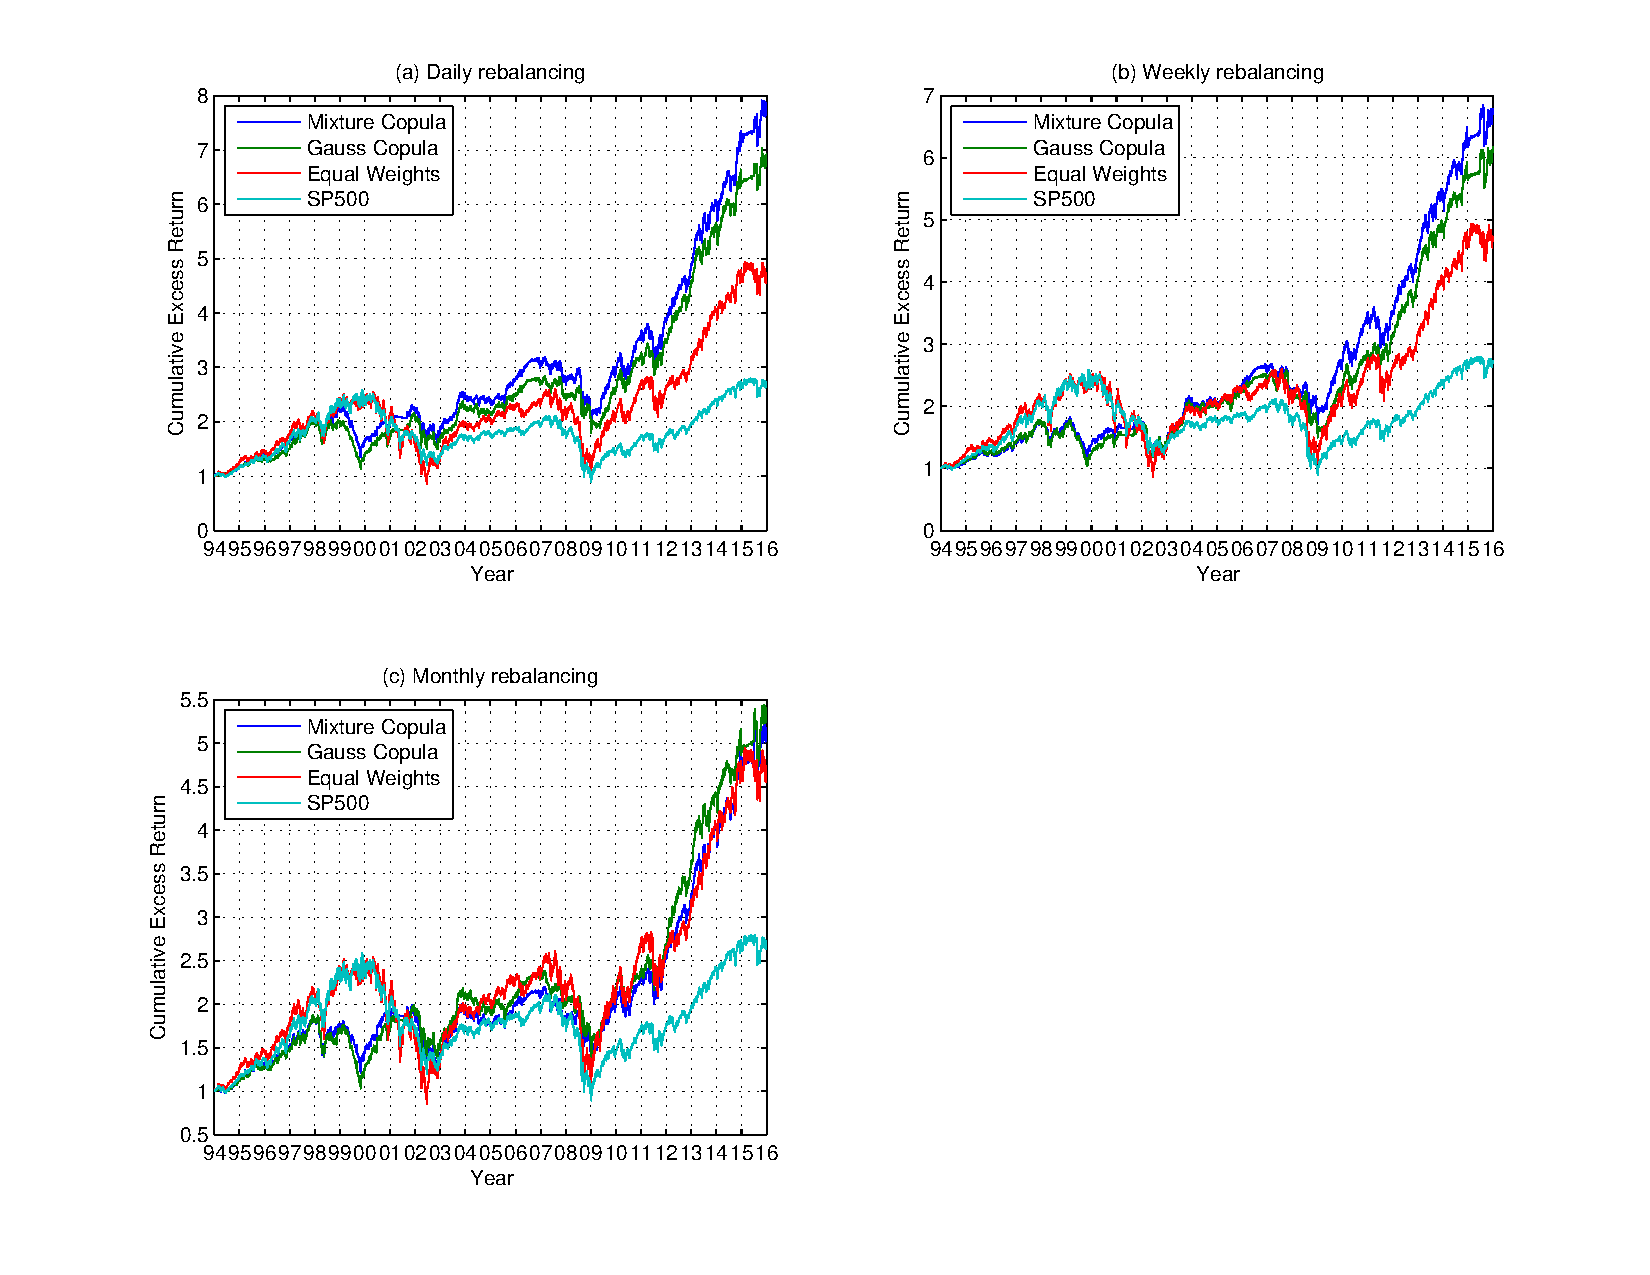
\includegraphics[width=\linewidth]{fig1_rpwcop.pdf}
	\captionsetup{justification=raggedright,
		singlelinecheck=false
	}
	\caption*{Source: Author's own elaboration (2017).}
	\caption*{This figure shows how an investment of \$1 evolves from July 1994 to December 2015 for each of the portfolios.}
	\label{fig:fig01}
\end{figure}

The copula-based approaches are more profitable for daily and weekly rebalancing over time, especially after 2009. We can note the copula methods present a hump-shaped pattern in 1999, while the other benchmarks show a sharp decline in the subperiod that corresponds to the bear market that comprises the dotcom crisis and the September 11th terrorist attack (2000-2002). All portfolios show a hump-shaped pattern during the subprime mortgage financial crisis in 2007-2008. Overall, we can observe that after 2002 the patterns are similar, but the figure indicates that the copula methods, even though the objective function is the minimization of CVaR under a constraint on expected return, preserve more wealth in the long-term period, particularly the WCCVaR portfolio, for daily and weekly rebalancing \footnote{Transaction costs should not be neglected as we could notice after the breakeven analysis}.



\vspace{0.3cm}


\section{Conclusions}

In this paper we combine robust portfolio optimization and copula-based models in a Worst Case CVaR framework. To cope with the large number of financial instruments we employ a procedure similar to that used by \citet*{ggr06} to select a set of diversified assets that can be useful during crises and tranquil periods. Using data from the S\&P 500 stocks from 1990 to 2015 we evaluate the performance of the WCCVaR (Worst Case Copula-CVaR) portfolio, considering different rebalancing strategies, and compare it against three benchmarks: a Gaussian Copula-CVaR (GCCVaR) portfolio, an equally weighted portfolio (1/N) and the S\&P 500 index. 

By selecting a diversified set of assets over a long-term period we found that copula-based approaches offer better hedges against losses than the 1/N portfolio. Moreover, the WCCVaR approach generates portfolios with better downside risk statistics for any rebalancing period and it is more profitable than the Gaussian Copula-CVaR for daily and weekly rebalancing.

Finally, we offer some suggestions for future research for improving our discoveries. First, we could improve the method of asset selection. We suspect that if we use a measure of nonlinear dependence between random variables of arbitrary dimension such as the randomized dependency coefficient (\citet*{lopez2013randomized}) or a procedure based on data mining tools as random forest \citet*{dlrz10} to select the stocks the portfolio performances would be even better. 
Additional suggestions include relaxing the assumption of no short selling and incorporate transaction cost as an additional constraint in the optimization problem as in \citet*{krokhmal2002}.

\addcontentsline{toc}{section}{References}
%\bibliographystyle{rfs}
%\bibliography{mypapers}
\printbibliography[title={REFERENCES}]
\end{refsection}
\newpage


\chapter{Performance of Copula-HEAVY, Copula-GARCH and Distance Pairs Trading on global stock market equity indices}
\thispagestyle{myheadings}
\markright{}


\pagestyle{myheadings}
\markright{}

%\begin{center}
%\Large \sc Nonparametric Frontier Estimation in Two Steps\normalsize \rm  \\[0.4in]
%\end{center}
%\begin{center}\sc Fernando A. Boeira Sabino da Silva,\footnote{Department of Statistics, Federal University of Rio Grande do Sul, Porto Alegre, RS 91509-900, Brazil, e-mail: fsabino@ufrgs.br} and Flavio A. Ziegelmann\footnote{Department of Statistics, Federal University of Rio Grande do Sul, Porto Alegre, RS 91509-900, Brazil, e-mail: flavioz@ufrgs.br} \end{center}
%\date{}                                           % Activate to display a given date or no date

%\begin{document}

\begin{refsection}
\renewcommand{\thetable}{\arabic{table}}

\setlength{\baselineskip}{12pt}
\noindent\bf Abstract. \rm By using an intra-day realized measure we empirically evaluate a Copula-HEAVY pairs trading model against a Copula-GARCH and the distance methods using 21 global stock market indices from January 2000 to June 2016. We find that Copula-GARCH approach is highly profitable with annual excess returns up to 12.10\% and 29.95\% on committed and fully invested capital, respectively, and Sharpe ratios up to 3.16. On the other hand, the Copula-HEAVY and distance methods show an annualized excess returns on committed and fully invested capital as high as 7.02\% and 17.19\% and 3.10\% and 3.62\%, and Sharpe ratios up to 2.21 and 0.6, respectively. The copula-based pairs strategies also present more trading opportunities than the distance strategies. However, the average excess returns of copula strategies are more sensitive to transaction costs and speed of execution. To test the statistical significance of the Sharpe Ratio and excess returns we adopt the stationary bootstrap of \citet*{pr94} using the automatic block-length selection of \citet*{pw04}. Results suggest that the Copula-GARCH is consistently the best rewarding strategy when a fast trade is made.\\[.1in]

\noindent \bf Keywords: \rm Pairs Trading. Copula. Distance. Statistical Arbitrage. High-Frequency. Realized variance. Stationary Bootstrap. \\[.1in]
\noindent \bf JEL Classifications. \rm  C51, C58, G11, G12, G14.
\clearpage

\setlength{\baselineskip}{12pt}
%\pagestyle{plain}
%\setcounter{page}{1}
\setcounter{footnote}{0}
\clearpage
\section{Introduction}
\label{introduction}

Pairs trading is a statistical arbitrage method that is often used by proprietary trading firms and hedge funds which exploits relative mispricing within two assets. The strategy attracts much interest in empirical finance, since it has potential to achieve abnormal returns through relatively low-risk positions. In addition, the strategy is claimed to be market neutral, which means that the investors are not exposed to market risk. The strategy was successfully pioneered by Gerry Bamberger and  Nunzio Tartaglia's quantitative group at Morgan Stanley in the 1980s \citet*{ggr06}. Since then many techniques to compute the spread between stock pairs were proposed; however, the strategy became popular through the study carried out by \citet*{ggr06}, named distance method.

In an efficient market, strategies based on mean-reversion concepts should not generate consistent profits. However, \citet*{ggr06} found that pairs trading generates consistent statistical arbitrage profits in the U.S. equity market during 1962-2002 using all liquid U.S. stocks from the Center for Research in Security Prices (CRSP) data, although the profitability declined over the period. They obtain an annual mean excess return above 11\% during the reported period. The authors attributed the abnormal returns to a non-identified systematic risk factor. They support their view by showing that there is a high degree of correlation between the excess returns of non-overlapping top pairs even after accounting for risk factors from an augmented version of \citet*{ff93}'s three-factor model. \citet*{df10} extend their work by expanding the data sample by more seven years and also found a declining trend (33 basis points (bps) mean excess return per month for 2003-09 versus 124 bps mean excess return per month for 1962-88). \citet*{df12} show that the distance method is unprofitable after 2002 when taking trading costs into account. \citet*{bv12} test the profitability of pairs trading under different weighting structures and trade initiation conditions using data from the Finnish stock market. They also found that their proposed strategy is profitable even after initiating the positions one day after the signal.

Currently, there are three main methods for pairs trading: distance, cointegration, and copula. The first two rely on the assumption that the pair of stocks is linearly associated which holds as long as the data have a multivariate normal distribution. However, it is well known that the dependence between two securities is rarely jointly normal \citep{campbell97,cont01,ane03,mcneil15} and thus a high-dimensional multivariate approach to tail dependence analysis is surely more insightful than assuming multivariate normal returns. Therefore, the trading signals based on the distance and cointegration strategies may fail to catch the dynamics of the spread between a pair of securities, and thus initiate and close the trades at non-optimal positions. To overcome these issues, \citet*{lw2013} propose a pairs trading strategy based on bivariate copulas. Because of its flexibility, copulas are able to model better the empirically verified non-linear relations normally attributed to multivariate financial returns such as asymmetric conditional variance with higher volatility for large negative returns and smaller volatility for positive returns \citep{h98} and leptokurdicity \citep{t01,andreou01}. However, they evaluate its performance using only three pre-selected pairs over a period of less than three years. \citet*{xie14} employ a similar methodology on a daily frequency over a ten-year period selecting 89 stocks from the U.S. utility sector. Both studies found that the copula-based strategy generates higher average excess returns and more trading opportunities than the distance approach. However, \citet*{rf15} found opposite results using daily U.S. equity data from 1962 to 2014. Particularly, the distance, cointegration, and Copula-GARCH strategies show an average monthly excess return of 36, 33, and 5 basis points (bps) after transaction costs, respectively, and 88, 83, and 43 bps before transaction costs, respectively.  All the aforementioned papers test the distance and copula strategies on daily frequency data and the dependence parameters of the copula-based approaches are assumed to be time-invariant.

However, currently there is no extensive research on pairs trading strategies using realized measures computed by employing higher frequency data. \citet*{nath2003high} employs a variant of the \citet*{ggr06}'s approach using intraday quotes from the U.S. treasury market from 1994 to 2000. He found that the strategy outperforms the benchmarks, especially regarding Sharpe Ratio. \citet*{bowen2010high} test the method using a 60-minute frequency in a sample of the FTSE 100 constituent stocks from January to December 2007. They document that the average excess returns of the strategy is very sensitive to trading costs and speed of execution. In particular, the profitability of the strategy for Top 5 pairs using 2.0$\sigma$ standard deviations is almost 20\% more before costs and it is reduced by almost 50\% when employing 10 basis points. In addition, when allowing a one-day waiting period restriction on execution, the profits are eliminated. They also describe that over a half of the excess returns is accomplished in the first hour of trading and 75\% in the first and last hours of the trading day. \citet*{dunis2010} test a cointegration pairs trading approach in intraday data of  5, 10, 20, 30 and 60 minutes in the constituent stocks of the Euro Stoxx 50 index comprising the period from 3rd July 2009 to 17th November 2009. They found an annualized average Information Ratio above 3 for high frequency intervals and about 1.3 using daily data for the Top 5 pairs.

Standard univariate GARCH models specify the conditional volatility as a function of past low-frequency data (\emph{i.e.}, daily returns). \citet*{andersen2001} show that underlying latent volatility can be computed accurately using intraday returns, whereas squared returns only provide a very noisy volatility indicator. It is shown that, when appropriately managed, incorporating realized volatility measures provides better volatility forecasts when compared to estimates constructed using daily data \citep{ss10,hansen2012realized}. \citet*{fleming2003} estimate that a risk-averse investor would be willing to pay 50 to 200 basis points per year to capture the observed gains in performance.

A class of univariate forecasting model that are based on realized measures of high frequency volatility is called High Frequency Based Volatility (HEAVY). It can be shown that the HEAVY model exhibits short-run momentum and mean-reversion effects, adjusting quickly to structural breaks in the level of the volatility process than standard GARCH models \citep{ss10}. Thus, by using realized information about current levels of volatilities, the HEAVY model may be particularly useful during periods of fast changes in the underlying volatility process. The realized measure we use here is a simple realized variance (RV) estimator with a 5-minute sample frequency, namely 5-minute realized variance. \citet*{liu2015does} show that there is little evidence that a 5-minute RV is outperformed by a profusion of other realized measures.

In this chapter, we conduct an empirical investigation in order to offer some evidence of the behavior of the Copula-HEAVY, Copula-GARCH, and distance pairs trading strategies under different investment scenarios using 21 global stock market indexes from January 2000 to June 2016. All data we use are obtained from Oxford-Man Institute of Quantitative Finance Realized Library\footnote{\url{http://realized.oxford-man.ox.ac.uk/data/download}}. We are also interested in providing some evidence of how the delay to start the positions as well the trading costs affects the profitability of these strategies. Our aim is to provide investors with information that allows for a more accurate selection of which strategy should be used in a particular setting and understand any differences in performance.

Our results indicate that the Copula-GARCH strategy outperforms consistently the other strategies for Top 20 pairs in the long term in terms of wealth accumulation and risk-adjusted returns when a fast trade can be executed assuming four equally spaced levels of transaction costs from zero to 15 basis points and before costs for a wait one-day rule. The Copula-HEAVY approach also outperforms the distance methods for transaction costs up to 10 basis points when positions are initiated and closed in the same day the pair diverges and converges, respectively. However, the returns from copula strategies are very sensitive to the magnitude of transaction costs and speed of execution. This is probably due to the fact we measure the degrees of relative mispricing for a single day instead of determining an overall degree of mispricing, increasing the number of trading opportunities.

To test the statistical significance of the returns and Sharpe Ratios we adopt the stationary bootstrap of \citet*{pr94} using the automatic block-length selection of \citet*{pw04} and 10,000 bootstrap resamples. To compute the bootstrap $p$-values we use the methodology proposed by \citet*{lw08}. Our objective is to compare the results on a statistical basis in order to mitigate potential data snooping problems. We find that the Copula-GARCH strategy significantly outperforms the other strategies (all p-values are less than 0.5\%) when a rapid trade is made.

Additionally, we conduct the analysis using four sub-periods to avoid the concern that the results are good only for the whole period: (1) January 2001 to December 2002; (2) January 2003 to June 2007; (3) July 2007 to June 2009, (4) and July 2009 to June 2016. The first sub-period corresponds to the bear market that spans the dotcom crisis and the September 11th terrorist attack. The third sub-period corresponds to the subprime mortgage financial crisis. Our results indicate that the copula methods achieve its best performance during financial downturns when trades can be quickly executed after the signal.

The remainder of this chapter is organized as follows. In Section 2 we briefly discuss the data and introduce the HEAVY model. In Section 3, we present the results of our empirical analysis. Finally, in Section 4, we conclude. The Appendix contains additional results.

\vspace{0.6cm}

\section{Data and the HEAVY model}
\label{section2}

Our data set consists of daily data of adjusted closing prices of 21 global stock market indexes obtained from the Oxford-Man Institute's realized library from January 2000 to June 2016. The data set sample period is made up of 4310 days and consists of the following indexes: S\&P 500, NASDAQ-100, FTSE 100, STI, Nikkei 225, Russell 2000, DAX-30, AORD, DJI, CAC40, HSI, KS11, AEX, SSMI, IBEX 35, Nifty 50, MXX, Ibovespa, S\&P/TSX, EURO STOXX 50, and FTSE MIB.

Our implementation of the pairs trading is similar to \citet*{ggr06} and is explained in more details in subsections 2.2.1 and 2.2.2. Potential security pairs are sorted based on the sum of squared differences in their normalized prices during the formation period. After the pairs are formed, their spread is monitored throughout the trading period and any deviations beyond a certain threshold in that spread would trigger the opening of two simultaneous long and short positions. However, as in \citet*{bv12}, we trade the pairs at the beginning of every six months, so we do not have a time series of overlapping six-month trading period as in \citet*{ggr06}. We use the distance approaches as our benchmarks and evaluate Copula-HEAVY and Copula-GARCH strategies by comparing their performance. As realized measure, we use realized variance at 5-minute intervals without sub-sampling.

Pairs are formed based on the smallest sum of squared deviations between the two normalized price deviations among all stocks listed throughout the 12 plus 6-month period (formation and trading periods) for both distance and copula approaches\footnote{%
	Missing values have been interpolated.}. For the distance method, the positions are initiated when this spread is greater than 0.75 and 2.0 standard deviations (based on \citet*{v04} and \citet*{ggr06}, respectively). If normally distributed, this would happen 45\% and 5\% approximately of the time, respectively. For the copula approach, we set 0.25 and 0.75 for the mispricing indexes. This would be similar to 0.75$\sigma$ trigger point if data is normally distributed.

\vspace{0.6cm}

\subsection{The HEAVY model}

Let us denote the time series of log daily return data and the realized 5-minute variance by $r_{1},r_{2},\ldots,r_{T}$ and $RV_{1},RV_{2},\ldots,RV_{T}$, respectively. With the realized measures computed for $T$ days, the HEAVY (High Frequency Based Volatility) model \citep{ss10} is given by:
\begin{align}
Var\left(r_{t}\left\vert\mathcal{F}_{t-1}^{HF}\right. \right)
&\equiv h_{t}=w_{H}+\alpha _{H}RV_{t-1}+\beta _{H}h_{t-1},  \label{CC} \\
E\left(RV_{t}\left\vert\mathcal{F}_{t-1}^{HF}\right. \right)  &\equiv \mu_{t}=w_{R}+\alpha_{R}RV_{t-1}+\beta_{R}\mu_{t-1},  \label{OC}
\end{align}
for $t=2,\ldots,T$, where $\mathcal{F}_{t-1}^{HF}$ stands for high-frequency information (intraday returns) from the previous day, and $w_{H},\alpha,w_{R},\alpha_{R},\beta_{R}\geq 0$, $\beta _{H}\in[0,1]$ and $\alpha_{R}+\beta_{R}\in[0,1]$ are stability conditions. The first equation models the known as close-to-close conditional variance and is alike to a standard GARCH model\footnote{The standard GARCH(1,1) is given by
	\begin{equation}
		Var\left(r_{t}\left\vert \mathcal{F}_{t-1}^{LF}\right. \right) =\sigma
	_{t}^{2}=w_{G}+\alpha_{G}r_{t-1}^{2}+\sigma_{t-1}^{2},
	\label{GCC}
	\end{equation}
	where $\mathcal{F}_{t-1}^{LF}$ denotes the low-frequency information (daily returns) from the previous day. The GARCH equation models the close-to-close conditional variance.}, whereas the second equation models the conditional expectation of the open-to-close variation\footnote{A Matlab code is available from Kevin Sheppard at \url{https://www.kevinsheppard.com/MFE_Toolbox}.}. The parameters estimates are obtained by using quasi-maximum likelihood.

The implementation of the Copula-HEAVY strategy is similar to the Copula-GARCH approach from subsection 2.2.2. In the first step, we fit an appropriate ARMA-HEAVY model\footnote{We look for the optimal ARMA(p,q) model up to order (1,1).} to each univariate time series (daily returns of the formation period) by obtaining the estimates $\widehat{\mu }_{i}$ and $\widehat{\sigma }_{i}$ of the conditional mean and variance of these processes, respectively. Moreover, using the estimated parametric models, we construct the standardized residuals vectors given, for each $i=1,...,t$, by
\begin{equation}
\begin{aligned}
\widehat{\varepsilon }_{i}=\frac{x_{i}-\widehat{\mu }_{i}}{\widehat{\sigma }_{i}}.
\end{aligned}
\label{eq:eq32}
\end{equation}

The standardized residuals vectors are then converted to the pseudo-observations $z_{i}=\frac{n}{n+1}F_{i}\left( \widehat{\varepsilon }_{i}\right) $, where $F_{i}$ is estimated by using their empirical distribution function. In the second step, with the estimated parameters from the previous step, we nominate the copula that best fits the uniform marginals and estimate its parameter(s). The copulas that are tested are Gaussian, Student's t, Clayton, Frank, Gumbel and one Archimedean mixture copula consisting of the best linear combination of Clayton, Frank and Gumbel copulas. We consider as the optimal copula the one with the lowest negative log-likelihood.

Finally, we follow the approach of \citet*{xie14} to obtain $MI_{X\mid Y}$ and $MI_{Y\mid X}$ as already described in subsection 2.2.2.

\vspace{0.6cm}

\section{Empirical Results}

An empirical study is carried out to evaluate and compare the performance of the distance and copula strategies. Such study is necessarily restrictive because there are many possibilities regarding the selection of the degree of pair-divergence, the trading costs, the number of pairs, the type of volatility model, the probability density functions, the method of pair selection, among other factors.

\vspace{0.3cm}

\subsection{Profitability of the Strategies}

Tables \ref{tab:table201} and \ref{tab:table202} exhibit annualized excess returns, annualized Sharpe and Sortino ratios, \citet*{nw87} adjusted t-statistics, share of negative observations, the maximum drawdown in terms of maximum percentage drop between two consecutive days (MDD1) and between two days within a period of maximum six months (MDD2) for each of the four strategies for from 2001-2016/1 assuming four equally spaced levels of transaction costs for Top 20 pairs. Table \ref{tab:table201} summarize results when positions are initiated and closed in the same day the pair diverges and Table \ref{tab:table202} when we delay trades by one day. Section 1 describes the Return on Committed Capital and Section 2 on Fully Invested Capital.

A series of important observations can be made from Table \ref{tab:table201}. First, notice that there exist strong evidence of the superiority of the Copula-GARCH strategy concerning the profitability of the strategies. The method yields an annual excess return up to 12.10\% and 29.95\% before costs on committed and fully invested capital, respectively and shows the highest Sharpe ratios (up to 3.16). Also note that the approach is the only strategy which delivers Sharpe ratios above 1 for all levels of transaction costs, indicating that investors are compensated for taking on additional risk. The Sortino ratio also confirms that the Copula-GARCH strategy delivers better risk-adjusted performance across-the-board. Second, we can observe that the excess returns from the model are always statistically and economically significant at 1\% (\citet*{nw87} adjusted t-statistics are between 5.94 and 13.57). Furthermore, the Copula-GARCH approach shows a lower probability of a negative trade and it also presents the best results on committed capital when we focus on capital preservation over a period of six months based on maximum drawdown (MDD2) measure.

The Copula-HEAVY strategy also shows a consistent better performance than the distance methods for transaction costs up to 10 basis points in terms of wealth accumulation, wealth preservation and risk-adjusted returns. However, the approach does not generated significant excess returns when we set the transaction costs to be 15 basis points. In this case the distance strategies show better results than the Copula-HEAVY approach, particularly for 0.75$\sigma$ trigger point.\\

\begin{threeparttable}[H]
	\centering \scriptsize \singlespacing
	\caption{Excess returns of pairs trading strategies on portfolios of Top 20 pairs without delay. }
	\begin{tabularx}{\textwidth}{@{\extracolsep{\fill}}llllllll@{}}
		\toprule
		Strategy & Mean  & Sharpe & Sortino & t-stat & \% of negative   & MDD1 & MDD2 \\
		& Return & ratio &  ratio     &  &  trades     &       &  \\
		\midrule
		\multicolumn{8}{c}{\textbf{Section 1: Return on Committed Capital}} \\
		\multicolumn{8}{c}{\textit{Panel A - Before Transaction Costs}} \\
		&       &       &       &       &       &       &  \\
		Distance (2.0$\sigma$) & 1.49 & 0.32 & 0.58 & $1.76^{*}$ & 49.80 & -2.55 & -6.25 \\
		Distance (0.75$\sigma$) & 3.10 & 0.57 & 1.06 & $2.99^{***}$ & 49.88 & -3.05 & -7.43 \\
		Copula-GARCH & 12.10 & 3.16 & 7.21 & $13.57^{***}$ & 42.99 & -2.37 & -2.70 \\
		Copula-HEAVY & 7.02 & 2.21 & 4.38 & $9.81^{***}$ & 44.35 & -2.34 & -3.30 \\
		\multicolumn{1}{r}{} & \multicolumn{1}{r}{} & \multicolumn{1}{r}{} & \multicolumn{1}{r}{} & \multicolumn{1}{r}{} & \multicolumn{1}{r}{} & \multicolumn{1}{r}{} & \multicolumn{1}{r}{} \\
		\multicolumn{8}{c}{\textit{Panel B - Transaction Costs: 5 basis points}} \\
		&       &       &       &       &       &       &  \\
		Distance (2.0$\sigma$) & 1.37  & 0.29  & 0.53  & 1.63  & 49.88 & -2.55  & -6.26 \\
		Distance (0.75$\sigma$) & 2.86  & 0.53  & 0.98  & $2.78^{***}$  & 50.07 & -3.05  & -7.52 \\
		Copula-GARCH & 10.05 & 2.68  & 5.99  & $11.52^{***}$ & 45.06 & -2.37  & -3.66 \\
		Copula-HEAVY & 4.82  & 1.55  & 2.98  & $6.90^{***}$  & 46.81 & -2.35  & -3.87 \\
		\multicolumn{1}{r}{} & \multicolumn{1}{r}{} & \multicolumn{1}{r}{} & \multicolumn{1}{r}{} & \multicolumn{1}{r}{} & \multicolumn{1}{r}{} & \multicolumn{1}{r}{} & \multicolumn{1}{r}{} \\
		\multicolumn{8}{c}{\textit{Panel C - Transaction Costs: 10 basis points}} \\
		&       &       &       &       &       &       &  \\
		Distance (2.0$\sigma$) & 1.25  & 0.27  & 0.49  & 1.50  & 49.95 & -2.55  & -6.29 \\
		Distance (0.75$\sigma$) & 2.62  & 0.48  & 0.90  & $2.56^{**}$  & 50.12 & -3.05  & -7.60 \\
		Copula-GARCH & 8.05  & 2.19  & 4.79  & $9.42^{***}$  & 47.23 & -2.38  & -4.38 \\
		Copula-HEAVY & 2.67  & 0.88  & 1.64  & $3.93^{***}$  & 49.83 & -2.37  & -4.58 \\
		\multicolumn{1}{r}{} & \multicolumn{1}{r}{} & \multicolumn{1}{r}{} & \multicolumn{1}{r}{} & \multicolumn{1}{r}{} & \multicolumn{1}{r}{} & \multicolumn{1}{r}{} & \multicolumn{1}{r}{} \\
		\multicolumn{8}{c}{\textit{Panel D - Transaction Costs: 15 basis points}} \\
		&       &       &       &       &       &       &  \\
		Distance (2.0$\sigma$) & 1.13  & 0.24  & 0.45  & 1.36  & 50.02 & -2.55  & -6.34 \\
		Distance (0.75$\sigma$) & 2.38  & 0.44  & 0.82  & $2.35^{**}$  & 50.22 & -3.06  & -7.69 \\
		Copula-GARCH & 6.08  & 1.69  & 3.61  & $7.27^{***}$  & 49.78 & -2.39  & -5.19 \\
		Copula-HEAVY & 0.58  & 0.19  & 0.37  & 0.91  & 52.47 & -2.38  & -5.54 \\
		\multicolumn{1}{r}{} & \multicolumn{1}{r}{} & \multicolumn{1}{r}{} & \multicolumn{1}{r}{} & \multicolumn{1}{r}{} & \multicolumn{1}{r}{} & \multicolumn{1}{r}{} & \multicolumn{1}{r}{} \\
		\midrule
		\multicolumn{8}{c}{\textbf{Section 2: Return on Fully Invested Capital}} \\
		\multicolumn{8}{c}{\textit{Panel A - Before Transaction Costs}} \\
		&       &       &       &       &       &       &  \\
		Distance (2.0$\sigma$) & 2.29 & 0.31 & 0.60 & $1.76^{*}$ & 49.80 & -3.61 & -8.49 \\
		Distance (0.75$\sigma$) & 3.62 & 0.58 & 1.10 & $3.00^{***}$ & 49.88 & -3.52 & -8.85 \\
		Copula-GARCH & 29.95 & 3.07 & 6.55 & $13.04^{***}$ & 42.99 & -4.24 & -6.96 \\
		Copula-HEAVY & 17.19 & 2.19 & 4.20 & $9.77^{***}$ & 44.35 & -3.86 & -9.68 \\
		\multicolumn{1}{r}{} & \multicolumn{1}{r}{} & \multicolumn{1}{r}{} & \multicolumn{1}{r}{} & \multicolumn{1}{r}{} & \multicolumn{1}{r}{} & \multicolumn{1}{r}{} & \multicolumn{1}{r}{} \\
		\multicolumn{8}{c}{\textit{Panel B - Transaction Costs: 5 basis points}} \\
		&       &       &       &       &       &       &  \\
		Distance (2.0$\sigma$) & 2.13  & 0.29  & 0.56  & $1.65^{*}$  & 49.88 & -3.61  & -8.50 \\
		Distance (0.75$\sigma$) & 3.35  & 0.54  & 1.02  & $2.79^{***}$  & 50.07 & -3.53  & -8.94 \\
		Copula-GARCH & 23.68 & 2.52  & 5.28  & $10.74^{***}$ & 45.06 & -4.25  & -8.40 \\
		Copula-HEAVY & 11.29 & 1.49  & 2.81  & $6.70^{***}$  & 46.77 & -3.88  & -10.93 \\
		\multicolumn{1}{r}{} & \multicolumn{1}{r}{} & \multicolumn{1}{r}{} & \multicolumn{1}{r}{} & \multicolumn{1}{r}{} & \multicolumn{1}{r}{} & \multicolumn{1}{r}{} & \multicolumn{1}{r}{} \\
		\multicolumn{8}{c}{\textit{Panel C - Transaction Costs: 10 basis points}} \\
		&       &       &       &       &       &       &  \\
		Distance (2.0$\sigma$) & 1.96  & 0.27  & 0.52  & 1.54  & 49.95 & -3.61  & -8.51 \\
		Distance (0.75$\sigma$) & 3.08  & 0.50  & 0.94  & $2.59^{***}$  & 50.12 & -3.53  & -9.04 \\
		Copula-GARCH & 17.72 & 1.96  & 4.04  & $8.37^{***}$  & 47.23 & -4.26  & -10.55 \\
		Copula-HEAVY & 5.70  & 0.78  & 1.46  & $3.57^{***}$  & 49.78 & -3.91  & -12.25 \\
		\multicolumn{1}{r}{} & \multicolumn{1}{r}{} & \multicolumn{1}{r}{} & \multicolumn{1}{r}{} & \multicolumn{1}{r}{} & \multicolumn{1}{r}{} & \multicolumn{1}{r}{} & \multicolumn{1}{r}{} \\
		\multicolumn{8}{c}{\textit{Panel D - Transaction Costs: 15 basis points}} \\
		&       &       &       &       &       &       &  \\
		Distance (2.0$\sigma$) & 1.80  & 0.24  & 0.48  & 1.42  & 50.02 & -3.62  & -8.53 \\
		Distance (0.75$\sigma$) & 2.81  & 0.45  & 0.86  & $2.38^{**}$  & 50.22 & -3.53  & -9.13 \\
		Copula-GARCH & 12.04 & 1.38  & 2.81  & $5.94^{***}$  & 49.68 & -4.28  & -12.84 \\
		Copula-HEAVY & 0.40  & 0.06  & 0.16  & 0.40  & 52.47 & -3.93  & -13.82 \\
		\multicolumn{1}{r}{} & \multicolumn{1}{r}{} & \multicolumn{1}{r}{} & \multicolumn{1}{r}{} & \multicolumn{1}{r}{} & \multicolumn{1}{r}{} & \multicolumn{1}{r}{} & \multicolumn{1}{r}{} \\
		\bottomrule
	\end{tabularx}%
	\begin{tablenotes}
		\item \textit{Note:} \scriptsize Summary statistics of the annualized excess returns, annualized Sharpe and Sortino ratios on portfolios of top 20 pairs between January 2001 and June 2016 (4050 observations). The positions are initiated in the same day the pair diverges. The t-statistics are computed using Newey-West standard errors with six-lag correction. The positions are initiated in the same day the pair diverges. The t-statistics are computed using Newey-West standard errors with a six-lag correction. The columns labeled MDD1 and MDD2 compute the largest drawdown in terms of maximum percentage drop between two consecutive days and between two days within a period of maximum six months, respectively.
		\item \scriptsize $^{\ast\ast\ast}$, $^{\ast\ast}$, $^{\ast}$ significant at 1\%, 5\% and 10\% levels. respectively.
		\item Source: Author's own elaboration (2016).
	\end{tablenotes}
	\label{tab:table201}%
\end{threeparttable}%

\vspace{0.6cm}

It should be noted that the excess returns of copula strategies are considerably more affected by increasing transactions costs. Overall, the average excess return of copula approaches are reduced by around 2\% on committed capital for each extra 5 basis points attached to trade. On the other hand, the distance strategies profits are reduced by less than 0.25\% for each 5 basis points added. Considering this trend, it would be required more than 25 basis points to make the Copula-GARCH model less profitable than the distance strategies.

\vspace{0.6cm}

\subsubsection{Speed of execution}

So far we have assumed that a trade can be started as soon as the trigger points are reached. However, one may face situations where the price of a stock bounces very quickly back and forth affecting how fast a trade can be executed. To investigate the robustness of our results to bid-ask bounce \citep{j90,jt95,conrad89} we follow \citet*{ggr06} and use a ``one-day rule'', \emph{i.e.}, we evaluate the performance of the strategies when positions are initiated on the day after the price divergence and closed on the day after the convergence.

Table \ref{tab:table202} displays that the copula strategies are, likewise after transaction costs, more sensitive to the speed of execution than the distance approaches. The Copula-GARCH model still shows a better performance than the other strategies and delivers profits before costs. However, the trading profits do not survive after costs. The 2.0$\sigma$ trigger point shows very modest and not significant profits over the period.

Thus, our results imply that a significant portion of the returns for copula approaches occur in the first day of trading and therefore may be due to bid-ask bounce. However, as highlighted by \citet*{ggr06}, it is difficult to quantify which portion of this reduction is due to bid-ask bounce and which portion is derived from the true mean reversion in prices because of fast market adjustment.

\medskip

\begin{threeparttable}[H]
	\centering \scriptsize \singlespacing
	\caption{Excess returns of pairs trading strategies on portfolios of Top 20 pairs with one day waiting period.}
	\begin{tabularx}{\textwidth}{@{\extracolsep{\fill}}llllllll@{}}
		\toprule
		Strategy & Mean  & Sharpe & Sortino & t-stat & \% of negative   & MDD1 & MDD2 \\
		& Return & ratio &  ratio     &  &  trades     &       &  \\
		\midrule
		\multicolumn{8}{c}{\textbf{Section 1: Return on Committed Capital}} \\
		\multicolumn{8}{c}{\textit{Panel A - Before Transaction Costs}} \\
		&       &       &       &       &       &       &  \\
		Distance (2.0$\sigma$) & 0.38  & 0.09  & 0.18  & 0.56  & 49.90 & -2.21  & -6.93 \\
		Distance (0.75$\sigma$) & 0.01  & 0.00  & 0.05  & 0.14  & 50.74 & -2.37  & -8.39 \\
		Copula-GARCH & 1.31  & 0.39  & 0.67  & $1.86^{*}$  & 49.21 & -2.04  & -5.75 \\
		Copula-HEAVY & -0.34 & -0.12 & -0.16 & -0.50 & 49.31 & -2.34  & -4.98 \\
		\multicolumn{1}{r}{} & \multicolumn{1}{r}{} & \multicolumn{1}{r}{} & \multicolumn{1}{r}{} & \multicolumn{1}{r}{} & \multicolumn{1}{r}{} & \multicolumn{1}{r}{} & \multicolumn{1}{r}{} \\
		\multicolumn{8}{c}{\textit{Panel B - Transaction Costs: 5 basis points}} \\
		&       &       &       &       &       &       &  \\
		Distance (2.0$\sigma$) & 0.26  & 0.06  & 0.13  & 0.42  & 49.98 & -2.21  & -7.01 \\
		Distance (0.75$\sigma$) & -0.22 & -0.04 & -0.03 & -0.10 & 50.84 & -2.37  & -8.53 \\
		Copula-GARCH & -0.54 & -0.16 & -0.24 & -0.67 & 52.54 & -2.07  & -6.61 \\
		Copula-HEAVY & -2.40 & -0.82 & -1.23 & $-3.95^{***}$ & 53.58 & -2.36  & -5.91 \\
		\multicolumn{1}{r}{} & \multicolumn{1}{r}{} & \multicolumn{1}{r}{} & \multicolumn{1}{r}{} & \multicolumn{1}{r}{} & \multicolumn{1}{r}{} & \multicolumn{1}{r}{} & \multicolumn{1}{r}{} \\
		\multicolumn{8}{c}{\textit{Panel C - Transaction Costs: 10 basis points}} \\
		&       &       &       &       &       &       &  \\
		Distance (2.0$\sigma$) & 0.14  & 0.03  & 0.09  & 0.28  & 50.05 & -2.21  & -7.08 \\
		Distance (0.75$\sigma$) & -0.44 & -0.09 & -0.11 & -0.34 & 50.94 & -2.37  & -8.66 \\
		Copula-GARCH & -2.36 & -0.72 & -1.12 & $-3.21^{***}$ & 55.16 & -2.10  & -7.51 \\
		Copula-HEAVY & -4.40 & -1.53 & -2.25 & $-7.36^{***}$ & 56.99 & -2.37  & -7.01 \\
		\multicolumn{1}{r}{} & \multicolumn{1}{r}{} & \multicolumn{1}{r}{} & \multicolumn{1}{r}{} & \multicolumn{1}{r}{} & \multicolumn{1}{r}{} & \multicolumn{1}{r}{} & \multicolumn{1}{r}{} \\
		\multicolumn{8}{c}{\textit{Panel D - Transaction Costs: 15 basis points}} \\
		&       &       &       &       &       &       &  \\
		Distance (2.0$\sigma$) & 0.02  & 0.00  & 0.04  & 0.13  & 50.10 & -2.21  & -7.16 \\
		Distance (0.75$\sigma$) & -0.67 & -0.14 & -0.19 & -0.59 & 51.14 & -2.37  & -8.79 \\
		Copula-GARCH & -4.15 & -1.28 & -1.99 & $-5.75^{***}$ & 57.48 & -2.13  & -8.46 \\
		Copula-HEAVY & -6.36 & -2.23 & -3.24 & $-10.71^{***}$ & 59.63 & -2.39  & -8.11 \\
		\multicolumn{1}{r}{} & \multicolumn{1}{r}{} & \multicolumn{1}{r}{} & \multicolumn{1}{r}{} & \multicolumn{1}{r}{} & \multicolumn{1}{r}{} & \multicolumn{1}{r}{} & \multicolumn{1}{r}{} \\
		\midrule
		\multicolumn{8}{c}{\textbf{Section 2: Return on Fully Invested Capital}} \\
		\multicolumn{8}{c}{\textit{Panel A - Before Transaction Costs}} \\
		&       &       &       &       &       &       &  \\
		Distance (2.0$\sigma$) & 0.50  & 0.07  & 0.18  & 0.54  & 49.95 & -4.01  & -10.87 \\
		Distance (0.75$\sigma$) & -0.21 & -0.04 & -0.02 & -0.05 & 50.35 &  -2.94  & -9.78 \\
		Copula-GARCH & 1.75  & 0.18  & 0.38  & 1.01  & 49.48 & -4.75  & -19.26 \\
		Copula-HEAVY & -2.79 & -0.27 & -0.34 & -0.98 & 49.21 & -6.19  & -16.80 \\
		\multicolumn{1}{r}{} & \multicolumn{1}{r}{} & \multicolumn{1}{r}{} & \multicolumn{1}{r}{} & \multicolumn{1}{r}{} & \multicolumn{1}{r}{} & \multicolumn{1}{r}{} & \multicolumn{1}{r}{} \\
		\multicolumn{8}{c}{\textit{Panel B - Transaction Costs: 5 basis points}} \\
		&       &       &       &       &       &       &  \\
		Distance (2.0$\sigma$) & 0.34  & 0.05  & 0.14  & 0.42  & 50.02 & -4.01  & -10.95 \\
		Distance (0.75$\sigma$) & -0.45 & -0.08 & -0.09 & -0.27 & 50.40 & -2.95  & -9.89 \\
		Copula-GARCH & -1.03 & -0.11 & -0.10 & -0.27 & 51.14 & -4.75  & -19.76 \\
		Copula-HEAVY & -5.17 & -0.51 & -0.71 & $-2.06^{**}$ & 51.80 & -6.19  & -17.55 \\
		\multicolumn{1}{r}{} & \multicolumn{1}{r}{} & \multicolumn{1}{r}{} & \multicolumn{1}{r}{} & \multicolumn{1}{r}{} & \multicolumn{1}{r}{} & \multicolumn{1}{r}{} & \multicolumn{1}{r}{} \\
		\multicolumn{8}{c}{\textit{Panel C - Transaction Costs: 10 basis points}} \\
		&       &       &       &       &       &       &  \\
		Distance (2.0$\sigma$) & 0.18  & 0.03  & 0.10  & 0.31  & 50.07 & -4.01  & -11.03 \\
		Distance (0.75$\sigma$) & -0.69 & -0.12 & -0.16 & -0.49 & 50.47 & -2.95  & -10.01 \\
		Copula-GARCH & -3.73 & -0.40 & -0.59 & -1.57 & 52.10 & -4.76  & -20.25 \\
		Copula-HEAVY & -7.49 & -0.74 & -1.08 & $-3.15^{***}$ & 52.86 & -6.19  & -18.52 \\
		\multicolumn{1}{r}{} & \multicolumn{1}{r}{} & \multicolumn{1}{r}{} & \multicolumn{1}{r}{} & \multicolumn{1}{r}{} & \multicolumn{1}{r}{} & \multicolumn{1}{r}{} & \multicolumn{1}{r}{} \\
		\multicolumn{8}{c}{\textit{Panel D - Transaction Costs: 15 basis points}} \\
		&       &       &       &       &       &       &  \\
		Distance (2.0$\sigma$) & 0.02  & 0.00  & 0.06  & 0.19  & 50.12 & -4.01  & -11.11 \\
		Distance (0.75$\sigma$) & -0.93 & -0.17 & -0.23 & -0.71 & 50.67 & -2.95  & -10.13 \\
		Copula-GARCH & -6.36 & -0.70 & -1.07 & $-2.88^{***}$ & 53.51 & -4.76  & -20.74 \\
		Copula-HEAVY & -9.76 & -0.98 & -1.45 & $-4.24^{***}$ & 54.10 & -6.19  & -19.48 \\
		\multicolumn{1}{r}{} & \multicolumn{1}{r}{} & \multicolumn{1}{r}{} & \multicolumn{1}{r}{} & \multicolumn{1}{r}{} & \multicolumn{1}{r}{} & \multicolumn{1}{r}{} & \multicolumn{1}{r}{} \\
		\bottomrule
	\end{tabularx}%
	\begin{tablenotes}
		\item \textit{Note:} \scriptsize  Summary statistics of the annualized excess returns, annualized Sharpe and Sortino ratios on portfolios of top 20 pairs between January 2001 and June 2016 (4050 observations). We assume a one day waiting period after the pair diverges. The t-statistics are computed using Newey-West standard errors with six-lag correction.  The columns labeled MDD1 and MDD2 compute the largest drawdown in terms of maximum percentage drop between two consecutive days and between two days within a period of maximum six months, respectively.
		\item \scriptsize $^{\ast\ast\ast}$, $^{\ast\ast}$, $^{\ast}$  significant at 1\%, 5\% and 10\% levels, respectively.
		\item Author's own elaboration (2016).
	\end{tablenotes}
	\label{tab:table202}%
\end{threeparttable}%

\vspace{0.6cm}

\medskip

Cumulative excess returns over the full data set for each of the strategies with no delay and with ``one day waiting rule'' are displayed in Figures \ref{fig:fig203}  and \ref{fig:fig204}, respectively. Panels (a) to (h) show the returns from zero to fifteen basis points as transaction costs on committed (left panels) and fully invested capital (right panels), respectively. The conclusions drawn from the graphical inspection of the results are consistent with our quantitative counterparts for the mean excess returns and t-statistics provided in Tables \ref{tab:table201} and \ref{tab:table202}, thus reinforcing our empirical findings.\\

\begin{figure}[H]
	\centering
	\caption{Cumulative excess returns of the pairs trading strategies on portfolios of Top 20 pairs with no delay}
	\includegraphics[width=\linewidth]{fig1_p2_rev.pdf}
	\captionsetup{justification=raggedright,
		singlelinecheck=false
	}
	\caption*{Source: Author's own elaboration (2016.)}
	\caption*{This figure shows how an investment of \$1 evolves from January 2001 to June 2016 for each of the strategies}
	\label{fig:fig203}
\end{figure}

\begin{figure}[H]
	\centering
	\caption{Cumulative excess returns of pairs trading strategies on portfolios of Top 20 pairs with one day waiting period}
	\includegraphics[width=\linewidth]{fig2_p2_rev.pdf}
	\captionsetup{justification=raggedright,
		singlelinecheck=false
	}
	\caption*{Source: Author's own elaboration (2016.)}
	\caption*{This figure shows how an investment of \$1 evolves from January 2001 to June 2016 for each of the strategies}
	\label{fig:fig204}
\end{figure}

\vspace{0.3cm}

\subsection{Trading statistics}

Table \ref{tab:table203} provides trading statistics. The average price deviation trigger for opening pairs are listed in the first row of the panel for each strategy. The positions typically opens when prices have diverged by 5.64\%, 3.15\%, 5.32\% and 5.23\% or more for 2.0$\sigma$, 0.75$\sigma$, Copula-GARCH and Copula-HEAVY strategies, respectively. It is noticeable that the copula approaches generate more trading opportunities than the distance strategies, \emph{i.e.}, the average number of pairs open per period is notably higher across the board for copula strategies. Furthermore, when using the copula framework, the pairs stay open for a shorter period. This is a very important finding, since every trading signal is an opportunity to profit. The average number of pairs traded per six-month period is at least 8.35 times more for our copula strategies than for the distance approaches considered here. In addition, under copula rules, each pair is held open, in average, 2.48 and 2.33 trading days, indicating that the copula approaches are short-term strategies. Meanwhile, the average holding period for the distance approaches is at least 2.37 trading months which indicate that the methods are medium-term strategies in this case.\\

\begin{threeparttable}[H]
	\centering \scriptsize
	\caption{Trading statistics.}
	\begin{tabularx}{\textwidth}{@{\extracolsep{\fill}}p{7cm}p{1cm}p{1cm}p{1cm}p{1cm}@{}}
		\toprule
		\multicolumn{1}{l}{Strategy} & Distance (2.0$\sigma$) & Distance (0.75$\sigma$) & Copula-GARCH & Copula-HEAVY \\
		\midrule
		Average price deviation trigger for opening pairs & 0.0564 & 0.0315 & 0.0532 & 0.0523 \\
		Total number of pairs opened & 758   & 1433   & 11965  & 13456 \\
		Average number of pairs traded per six-month period & 24.45 & 46.23 & 385.97 & 434.06 \\
		Average number of round-trip trades per pair & 1.22 & 2.31 & 19.30 & 21.70 \\
		~~Standard Deviation & 0.70 & 1.78 & 6.12 & 13.33 \\
		Average time pairs are open in days & 69.92 & 49.83 & 2.48 & 2.33 \\
		~~Standard Deviation & 44.49 & 47.37 & 2.32 & 3.13 \\
		Median time pairs are open in days & 65.5    & 30    & 2     & 1 \\			
		\bottomrule
	\end{tabularx}%
	\begin{tablenotes}
		\item \textit{Note:}\scriptsize Trading statistics for portfolio of top 20 pairs between January 2001 and June 2016 (31 periods). Pairs are formed over a 12-month period according to a minimum-distance criterion and then traded over the subsequent 6-month period. Average price deviation trigger for opening a pair is calculated as the price difference divided by the average of the prices.
		\item Source: Author's own elaboration (2016).
	\end{tablenotes}
	\label{tab:table203}%
\end{threeparttable}%

\vspace{1.0cm}

\subsection{Robustness Checks of the Performance of Excess Returns and Sharpe Ratios}

In order to mitigate data-snooping criticisms, we use the stationary bootstrap of \citet*{pr94} to compute the bootstrap p-values using the methodology proposed by \citet*{lw08}. 

We want to further investigate if the average excess return and the Sharpe Ratio of the Copula-GARCH method show a significative superior out-of-sample performance compared to the distance and Copula-HEAVY strategies. 

In order to construct the distributions we bootstrapped the original time series $B=10,000$ times. Our bootstrapped null distributions result from Theorem 2 of \citet*{pr94}. We select the optimal block length for the stationary bootstrap following \citet*{pw04}. As the optimal bootstrap block length is different for each strategy, we average the block lengths found to perform the comparisons. 

To test the hypotheses that the average excess returns and Sharpe Ratios of the Copula-GARCH (cg) model are equal to that of distance (d) and Copula-HEAVY (ch) approaches, that is,
\begin{equation}
H_{0}:\mu_{cg}-\mu_{d}=0  \ \ \textrm{and}
\ \  H_{0}:\frac{\mu_{cg}}{\sigma_{cg}}-\frac{\mu_{d}}{\sigma_{d}}=0,
\label{eq:eq153}
\end{equation} 
and
\begin{equation}
H_{0}:\mu_{cg}-\mu_{ch}=0  \ \ \textrm{and}
\ \  H_{0}:\frac{\mu_{cg}}{\sigma_{cg}}-\frac{\mu_{ch}}{\sigma_{ch}}=0,
\label{eq:eq154}
\end{equation} we compute, following \citet*{davison1997}, a two-sized $p$-value using $B=10000$ (stationary) bootstrap re-samples. 

Table \ref{tab:table204} provides the bootstrap p-values for testing the null hypotheses represented by (\ref{eq:eq153}) and (\ref{eq:eq154}). Sections 1 and 2 compare the Copula-GARCH strategy to the 2.0$\sigma$ and 0.75$\sigma$ trigger points, respectively, and Section 3 to the Copula-HEAVY approach from 2001-2016/1 for all investment scenarios, \emph{i.e.}, without delay and waiting one day period and before and after costs.

As can be deduced from Table \ref{tab:table204} the Copula-GARCH model significantly outperforms the distance strategies when positions are initiated and closed in the same day the pair diverges (p-values < 0.5\%) for both weighting structures. On the other hand, the distance methods provide profits and Sharpe ratios significantly higher for wait one-day rule and 15 basis points at least at 10\% for both weighting schemes. The Copula-GARCH method also show a significant superior performance compared to the Copula-HEAVY approach (p-values less than 0.0001) when a fast execution of the trade can be made and for one-day waiting trading strategy on committed capital, at least at 5\%.

\vspace{0.3cm}

\begin{threeparttable}[H]
	\centering \scriptsize
	\caption{Bootstrap p-values computed from B=10,000 replications for testing the null hypotheses of equality of the average excess returns and Sharpe Ratios over the period between January 2001 and June 2016.}
	\begin{tabularx}{\textwidth}{@{\extracolsep{\fill}}lllllll@{}}
		\toprule
		& & \multicolumn{2}{c}{Committed Capital} & \multicolumn{1}{c}{} & \multicolumn{2}{c}{Fully Invested Capital} \\
		\cmidrule{3-4}  \cmidrule{6-7}
		\multicolumn{1}{c}{Scenario} & & \multicolumn{1}{c}{Return} & Sharpe Ratio &       & \multicolumn{1}{c}{Return}& Sharpe Ratio \\
		\midrule
		& \multicolumn{6}{c}{Section 1: Copula-GARCH versus 2.0$\sigma$} \\
		\midrule
		d0c0 & & $0.0000^{***}(>)$ & $0.0000^{***}(>)$ &       & $0.0000^{***}(>)$ & $0.0000^{***}(>)$ \\
		d0c5 & & $0.0000^{***}(>)$ & $0.0000^{***}(>)$ &       & $0.0000^{***}(>)$ & $0.0000^{***}(>)$   \\
		d0c10 & & $0.0000^{***}(>)$ & $0.0000^{***}(>)$ &       & $0.0000^{***}(>)$ & $0.0000^{***}(>)$ \\
		d0c15 & & $0.0006^{***}(>)$ & $0.0000^{***}(>)$ &       & $0.0000^{***}(>)$ & $0.0000^{***}(>)$ \\
		d1c0 & & 0.3900 & 0.2792  &       & 0.5748 & 0.6934 \\
		d1c5 & & 0.4036 & 0.3918 &       & 0.6358 & 0.6130 \\
		d1c10 & & $0.0134^{**}(<)$ & $0.0062^{***}(<)$ &       & 0.1258 & 0.1522 \\
		d1c15 & & $0.0000^{***}(<)$ & $0.0000^{***}(<)$ &       & $0.0096^{***}(<)$ & $0.0186^{**}(<)$ \\
		\midrule
		& \multicolumn{6}{c}{Section 2: Copula-GARCH versus 0.75$\sigma$} \\
		\midrule
		d0c0 & & $0.0000^{***}(>)$ & $0.0000^{***}(>)$ &       & $0.0000^{***}(>)$ & $0.0000^{***}(>)$ \\
		d0c5 & & $0.0000^{***}(>)$ & $0.0000^{***}(>)$ &       & $0.0000^{***}(>)$ & $0.0000^{***}(>)$   \\
		d0c10 & & $0.0000^{***}(>)$ & $0.0000^{***}(>)$ &       & $0.0000^{***}(>)$ & $0.0000^{***}(>)$ \\
		d0c15 & & $0.0048^{***}(>)$ & $0.0000^{***}(>)$ &       & $0.0000^{***}(>)$ & $0.0008^{***}(>)$ \\
		d1c0 & & 0.2562 & 0.1510  &       & 0.3490 & 0.4118 \\
		d1c5 & & 0.7138 & 0.6324 &       & 0.9116 & 0.9874 \\
		d1c10 & & $0.0620^{*}(<)$ & $0.0182^{**}(<)$ &       & 0.2284 & 0.3592 \\
		d1c15 & & $0.0010^{***}(<)$ & $0.0000^{***}(<)$ &       & $0.0218^{**}(<)$ & $0.0704^{*}(<)$ \\
		\midrule
		& \multicolumn{6}{c}{Section 3: Copula-GARCH versus Copula-HEAVY} \\
		\midrule
		d0c0 & & $0.0000^{***}(>)$ & $0.0000^{***}(>)$ &       & $0.0000^{***}(>)$ & $0.0000^{***}(>)$ \\
		d0c5 & & $0.0000^{***}(>)$ & $0.0000^{***}(>)$ &       & $0.0000^{***}(>)$ & $0.0000^{***}(>)$   \\
		d0c10 & & $0.0000^{***}(>)$ & $0.0000^{***}(>)$ &       & $0.0000^{***}(>)$ & $0.0000^{***}(>)$ \\
		d0c15 & & $0.0000^{***}(>)$ & $0.0000^{***}(>)$ &       & $0.0000^{***}(>)$ & $0.0000^{***}(>)$ \\
		d1c0 & & $0.0134^{**}(>)$  & $0.0138^{**}(>)$  &       & $0.0826^{*}(>)$  & $0.0820^{*}(>)$ \\
		d1c5 & & $0.0028^{***}(>)$ & $0.0010^{***}(>)$ &       & 0.1026 & 0.1250 \\
		d1c10 & & $0.0010^{***}(>)$ & $0.0000^{***}(>)$ &       & 0.1246 & 0.1940 \\
		d1c15 & & $0.0000^{***}(>)$ & $0.0000^{***}(>)$ &       & 0.1650 & 0.2920 \\
		\bottomrule
	\end{tabularx}%
	\begin{tablenotes}
		\item \textit{Note:} \scriptsize This table reports the bootstrap p-values for testing the null hypothesis of equality of the average excess returns and the Sharpe Ratios of Copula-GARCH and distance and Copula-HEAVY strategies for Top 20 pairs over the period between January 2001 and June 2016 (4050 observations). The column labeled Scenario contains symbol labels for trading with no delay or one day waiting period (d0 and d1, respectively) and before or after costs (c0, c5, c10 and c15, respectively). The symbol labels (>) and (<) indicate that the respective null hypothesis is rejected in favor of the alternative and that the average excess returns and/or the Sharpe Ratio of the Copula-GARCH strategy are found greater or less than the the average excess returns and/or the Sharpe Ratio of the distance and Copula-HEAVY strategies, respectively.
		\item \scriptsize $^{\ast\ast\ast}$, $^{\ast\ast}$, $^{\ast}$ significant at 1\%, 5\% and 10\% levels, respectively.
		\item Author's own elaboration (2016).
	\end{tablenotes}
	\label{tab:table204}%
\end{threeparttable}%

\vspace{1.0cm}

\subsection{Sub-period analysis}

Due to the sample horizon over 15 years, a sub-period analysis is inevitable to examine whether the profitability pattern has changed over time. We split the full sample period into four subperiods: (1) January 2001 to December 2002, (2) January 2003 to June 2007, (3) July 2007 to June 2009, and (4) July 2009 to June 2016. The first subperiod corresponds to the bear market that comprises the dotcom crisis and the September 11th terrorist attack. The third subperiod corresponds to the global financial crisis.

Figures \ref{fig:fig205} to \ref{fig:fig208} show annualized excess returns and Sharpe ratios of the four strategies for each subperiod with no delay and one-day waiting period, respectively. Panels (a) to (h) show the returns from zero to fifteen basis points as transaction costs on committed (left panels) and fully invested capital (right panels), respectively. 

As can be discerned analyzing figures \ref{fig:fig205} and \ref{fig:fig207} the Copula-GARCH strategy is consistently the most profitable approach among the four strategies and which produces the highest risk-adjusted returns with no delay to execute the required trades for both weighting structures. Moreover, it is remarkable that the Copula-GARCH method achieves its best performance over the two periods of higher stock market volatility, \emph{i.e.}, during financial downturns that comprise the first and the third subperiods. This is a desirable finding for a market neutral strategy. In addition, the Copula-GARCH method shows Sharpe ratios always above 2.5 over these two subperiods (they range between 2.56 and 3.92 for January 2001 to December 2002 and between 3.46 and 4.55 during the subprime mortgage crisis).

Further, as can be seen from figures \ref{fig:fig205} and \ref{fig:fig207}, the Copula-HEAVY and the 0.75 standard deviation approaches also achieve their best results during the subperiods of higher volatility, although the magnitude of the gains are relatively smaller for the distance strategy during the subprime mortgage crisis. 

\begin{figure}[H]
	\centering
	\caption{Average excess returns of pairs trading strategies for each subperiod with no delay}
	\includegraphics[width=\linewidth]{fig3_p2_rev.pdf}
	\captionsetup{justification=raggedright,
		singlelinecheck=false
	}
	\caption*{Source: Author's own elaboration (2016.)}
	%\caption*{comments}
	\label{fig:fig205}
\end{figure}

\begin{figure}[H]
	\centering
	\caption{Sharpe Ratio (annualized) of pairs trading strategies for each subperiod with no delay}
	\includegraphics[width=\linewidth]{fig5_p2_rev.pdf}
	\captionsetup{justification=raggedright,
		singlelinecheck=false
	}
	\caption*{Source: Author's own elaboration (2016.)}
	%\caption*{comments}
	\label{fig:fig207}
\end{figure}


Figures \ref{fig:fig206} and \ref{fig:fig208} show annualized excess returns and Sharpe ratios of the four strategies for each subperiod with one-day waiting period rule. As can be seen the Copula-HEAVY and the distance strategies are clearly more profitable in the first subperiod. However, there is a substantial decrease of profitability and risk-adjusted returns during the global financial crisis. Hence, it can be deduced that a significant part of the returns of the strategies occur in the first day of trading.

\begin{figure}[H]
	\centering
	\caption{Average excess returns of pairs trading strategies for each subperiod with one day waiting period}
	\includegraphics[width=\linewidth]{fig4_p2_rev.pdf}
	\captionsetup{justification=raggedright,
		singlelinecheck=false
	}
	\caption*{Source: Author's own elaboration (2016.)}
	%\caption*{comments}
	\label{fig:fig206}
\end{figure}

\begin{figure}[H]
	\centering
	\caption{Sharpe Ratio (annualized) pairs trading strategies for each subperiod with one day waiting period}
	\includegraphics[width=\linewidth]{fig6_p2_rev.pdf}
	\captionsetup{justification=raggedright,
		singlelinecheck=false
	}
	\caption*{Source: Author's own elaboration (2016.)}
	%\caption*{comments}
	\label{fig:fig208}
\end{figure}

\vspace{0.3cm}

Robustness checks of the performance of annualiazed excess returns and Sharpe ratios over the four subperiods are presented in in Tables \ref{tab:table206}-\ref{tab:table209} in the Appendix.

The results appear to remain consistent over the subperiods enhancing that the Copula-GARCH pairs strategy outperforms the other strategies when we initiate and close positions in the same day the pair diverges and converges, respectively.

\vspace{0.6cm}

\section{Conclusions}

The main objective of this chapter is to compare alternative copula pairs trading estimation procedures to understand better the factors that affect the profitability of the strategies. The main findings are summarized below.

\begin{enumerate}
	\item Results suggest that the Copula-GARCH pairs trading strategy is consistently the best rewarding strategy when a fast trade can be made.
	\item The Copula-HEAVY pairs trading strategy also shows a consistent better performance than the distance strategies for transaction costs up to 10 basis points in terms of wealth accumulation, wealth preservation and risk-adjusted returns when positions are initiated and closed in the same day the pair diverges and converges, respectively. 
	\item Results suggest that in the whole sample period the high-frequency based volatility model does not produce higher mean excess returns than the standard GARCH(1,1) model. It is possible that the estimation of more parameters leads to high estimation errors and therefore false transaction signals, thus decreasing the profitability of the Copula-HEAVY method.
	\item The excess returns from the Copula-GARCH method are always statistically and economically significant at 1\% when a fast execution of the trade can be made for all levels of transaction costs in this study. For the Copula-HEAVY approach the excess returns are not significant when the transaction costs are set to 15 basis points. 
	\item The Copula-GARCH strategy shows a lower probability of a trade with negative returns compared to the other approaches and it also displays the best results on committed capital when we focus on a steady performance and capital preservation over a period of six months.
	\item Without delay to start and close the positions the Copula-GARCH approach is the only strategy which produces Sharpe ratios above 1 for all levels of transaction costs, indicating that investors are compensated for taking on additional risk. The subperiod analysis also endorses that the strategy yields better risk-adjusted performance.
	\item The copula-based pairs strategies also present more trading opportunities than the distance strategies. However, the average excess returns of copula strategies are more sensitive to timing and transaction costs. When allowing a one-day waiting period restriction on execution, the profits of the copula-based pairs strategy are eliminated after costs. Hence, it can be deduced that a 
	significant part of the returns of the strategies occur in the first day of trading.
	\item It is remarkable that the copula approaches achieved its very best performance over periods of higher volatility, \emph{i.e.}, during financial downturns. This is a desirable finding for a market neutral strategy.
	\item The copula approaches are able to identify more trading opportunities than the distance strategies. Moreover, when using the copula methods the pairs stay open for a shorter period of time. This is a very important finding, since every trading signal is an opportunity to profit.
	
\end{enumerate}

\vspace{0.3cm}

Finally, we provide some suggestions for future research to improve our findings. First, we must become the comparisons more reliable and meaningful making the number of tradeable signals more comparable. We should investigate an overall degree of relative mispricing as in \citet*{rf15}. Second, in one attempt to understand the economic drivers behind our data and to evaluate whether the profitability is a compensation for risk, we could regress daily excess return onto various asset pricing factors (see \citet*{fama2012}). Third, we could employ a mixed copula model to cover a wider range of possible dependencies structures. Fourth, we could create similar copula-based arbitrage for triplets to increase information dependency information and measure relative pricing more comprehensively. Fifth, we could borrow some ideas from statistical learning and perform a model validation during the formation period. After choosing the pairs, we could check its predictive power by splitting data into two subsets. The idea is to select and fit the model based entirely on one part of the data, and then test it on the remaining part. Sixth, we could improve the method of pairs selection before using the copula approach. Since copulas capture better nonlinear dependence structures, we suspect that if we use a nonlinear association measurement such as the randomized dependency coefficient (Lopez-Paz et al., 2013), or a procedure based on data mining tools as random forest (Giovanni De Luca and Zuccolotto, 2010) to select the pairs, the performance of the copula method may be enhanced.

\addcontentsline{toc}{section}{References}
%\bibliographystyle{rfs}
%\bibliography{mypapers}
\printbibliography[title={REFERENCES}]
\end{refsection}


\newpage
\section*{Appendix A - Robustness Checks}
\addcontentsline{toc}{section}{Appendix A -  Robustness Checks}

Tables contain the results of robustness checks over the four subperiods. 

\setcounter{table}{0}
\renewcommand{\thetable}{A.\arabic{table}}

\begin{threeparttable}[H]
	\centering \scriptsize
	\caption{Bootstrap p-values computed from B=10,000 replications for testing the null hypotheses of equality of the average excess returns and Sharpe Ratios over the period between January 2001 and June 2002.}
	\begin{tabularx}{\textwidth}{@{\extracolsep{\fill}}lllllll@{}}
		\toprule
		& & \multicolumn{2}{c}{Committed Capital} & \multicolumn{1}{c}{} & \multicolumn{2}{c}{Fully Invested Capital} \\
		\cmidrule{3-4}  \cmidrule{6-7}
		\multicolumn{1}{c}{Scenario} & & \multicolumn{1}{c}{Return} & Sharpe Ratio &       & \multicolumn{1}{c}{Return}& Sharpe Ratio \\
		\midrule
		& \multicolumn{6}{c}{Section 1: Copula-GARCH versus 2.0$\sigma$} \\
		\midrule
		d0c0 & & $0.0022^{***}(>)$ & $0.0000^{***}(>)$ &       & $0.0046^{***}(>)$ & $0.0028^{***}(>)$ \\
		d0c5 & & $0.0084^{***}(>)$ & $0.0006^{***}(>)$ &       & $0.0158^{**}(>)$ & $0.0084^{***}(>)$   \\
		d0c10 & & $0.0306^{**}(>)$ & $0.0028^{***}(>)$ &       & $0.0544^{*}(>)$ & $0.0318^{**}(>)$ \\
		d0c15 & & 0.1068 & $0.0152^{**}(>)$ &       & 0.1438 & $0.0898^{*}(>)$ \\
		d1c0 & & 0.2906 & 0.1600  &       & 0.7338 & 0.8582 \\
		d1c5 & & 0.5048 & 0.3252 &       & 0.9454 & 0.9402 \\
		d1c10 & & 0.7614 & 0.5726 &       & 0.8950 & 0.7920 \\
		d1c15 & & 0.9320 & 0.9036 &       & 0.6904 & 0.6168 \\
		\midrule
		& \multicolumn{6}{c}{Section 2: Copula-GARCH versus 0.75$\sigma$} \\
		\midrule
		d0c0 & & $0.0714^{*}(>)$ & $0.0000^{***}(>)$ &       & $0.0006^{***}(>)$ & $0.0036^{***}(>)$ \\
		d0c5 & & 0.1622 & $0.0022^{***}(>)$ &       & $0.0040^{***}(>)$ & $0.0114^{**}(>)$   \\
		d0c10 & & 0.2768 & $0.0064^{***}(>)$ &       & $0.0164^{**}(>)$ & $0.0408^{**}(>)$ \\
		d0c15 & & 0.4706 & $0.0226^{**}(>)$ &       & $0.0562^{*}(>)$ & 0.1128 \\
		d1c0 & & 0.4744 & 0.1304  &       & 0.4578 & 0.7448 \\
		d1c5 & & 0.7210 & 0.3012 &       & 0.6228 & 0.9024 \\
		d1c10 & & 0.9850 & 0.5594  &       & 0.8278 & 0.9150 \\
		d1c15 & & 0.6986 & 0.9022 &       & 0.9832 & 0.7670 \\
		\midrule
		& \multicolumn{6}{c}{Section 3: Copula-GARCH versus Copula-HEAVY} \\
		\midrule
		d0c0 & & $0.0068^{***}(>)$ & $0.0136^{**}(>)$ &       & 0.1020 & 0.1156 \\
		d0c5 & & $0.0040^{***}(>)$ & $0.0086^{***}(>)$ &       & 0.1006 & 0.1056   \\
		d0c10 & & $0.0040^{***}(>)$ & $0.0066^{***}(>)$ &       & $0.0862^{*}(>)$ & $0.0868^{*}(>)$ \\
		d0c15 & & $0.0044^{***}(>)$ & $0.0052^{***}(>)$ &       & $0.0954^{*}(>)$ & $0.0914^{*}(>)$ \\
		d1c0 & & $0.0004^{***}(>)$  & $0.0004^{***}(>)$  &       & 0.1846  & 0.1508 \\
		d1c5 & & $0.0004^{***}(>)$ & $0.0004^{***}(>)$ &       & 0.2116 & 0.1882 \\
		d1c10 & & $0.0008^{***}(>)$ & $0.0010^{***}(>)$ &       & 0.2226 & 0.2004 \\
		d1c15 & & $0.0004^{***}(>)$ & $0.0004^{***}(>)$ &       & 0.2292 & 0.2196 \\
		\bottomrule
	\end{tabularx}%
	\begin{tablenotes}
		\item \textit{Note:} \scriptsize This table reports the bootstrap p-values for testing the null hypothesis of equality of the average excess returns and the Sharpe Ratios of Copula-GARCH and distance and Copula-HEAVY strategies for Top 20 pairs over the period between January 2001 and December 2002 (520 observations). The column labeled Scenario contains symbol labels for trading with no delay or one day waiting period (d0 and d1, respectively) and before or after costs (c0, c5, c10 and c15, respectively). The symbol labels (>) and (<) indicate that the respective null hypothesis is rejected in favor of the alternative and that the average excess returns the Sharpe Ratio of the Copula-GARCH strategy are found greater or less than the the average excess returns and/or the Sharpe Ratio of the distance and Copula-HEAVY strategies, respectively.
		\item \scriptsize $^{\ast\ast\ast}$, $^{\ast\ast}$, $^{\ast}$ significant at 1\%, 5\% and 10\% levels, respectively.
		\item Author's own elaboration (2016).
	\end{tablenotes}
	\label{tab:table206}%
\end{threeparttable}%

\vspace{1.0cm}

\begin{threeparttable}[H]
	\centering \scriptsize
	\caption{Bootstrap p-values computed from B=10000 replications for testing the null hypotheses of equality of the average excess returns and Sharpe Ratios over the period between January 2003 and June 2007.}
	\begin{tabularx}{\textwidth}{@{\extracolsep{\fill}}lllllll@{}}
		\toprule
		& & \multicolumn{2}{c}{Committed Capital} & \multicolumn{1}{c}{} & \multicolumn{2}{c}{Fully Invested Capital} \\
		\cmidrule{3-4}  \cmidrule{6-7}
		\multicolumn{1}{c}{Scenario} & & \multicolumn{1}{c}{Return} & Sharpe Ratio &       & \multicolumn{1}{c}{Return}& Sharpe Ratio \\
		\midrule
		& \multicolumn{6}{c}{Section 1: Copula-GARCH versus 2.0$\sigma$} \\
		\midrule
		d0c0 & & $0.0000^{***}(>)$ & $0.0000^{***}(>)$ &       & $0.0000^{***}(>)$ & $0.0000^{***}(>)$ \\
		d0c5 & & $0.0010^{***}(>)$ & $0.0000^{***}(>)$ &       & $0.0000^{***}(>)$ & $0.0000^{***}(>)$   \\
		d0c10 & & $0.0176^{**}(>)$ & $0.0008^{***}(>)$ &       & $0.0022^{***}(>)$ & $0.0022^{***}(>)$ \\
		d0c15 & & 0.2162 & $0.0622^{*}(>)$ &       & 0.1254 & 0.1256 \\
		d1c0 & & 0.2756 & 0.1716  &       & 0.4100 & 0.3882 \\
		d1c5 & & 0.9218 & 0.8570 &       & 0.9550 & 0.8878 \\
		d1c10 & & 0.1788 & $0.0728^{*}(<)$ &       & 0.4678 & 0.5444 \\
		d1c15 & & $0.0134^{**}(<)$ & $0.0004^{***}(<)$ &       & 0.1218 & 0.1774 \\
		\midrule
		& \multicolumn{6}{c}{Section 2: Copula-GARCH versus 0.75$\sigma$} \\
		\midrule
		d0c0 & & $0.0000^{***}(>)$ & $0.0000^{***}(>)$ &       & $0.0000^{***}(>)$ & $0.0000^{***}(>)$ \\
		d0c5 & & $0.0016^{***}(>)$ & $0.0000^{***}(>)$ &       & $0.0000^{***}(>)$ & $0.0000^{***}(>)$   \\
		d0c10 & & $0.0270^{**}(>)$ & $0.0010^{***}(>)$ &       & $0.0008^{***}(>)$ & $0.0036^{***}(>)$ \\
		d0c15 & & 0.2358 & $0.0518^{*}(>)$ &       & 0.1592 & 0.2068 \\
		d1c0 & & 0.1122 & $0.0664^{*}(>)$  &       & 0.4092 & 0.3638 \\
		d1c5 & & 0.6222 & 0.8090 &       & 0.9752 & 0.8340 \\
		d1c10 & & 0.5658 & 0.1946 &       & 0.4272 & 0.6156 \\
		d1c15 & & 0.1040 & $0.0032^{***}(<)$ &       & 0.1118 & 0.2272 \\
		\midrule
		& \multicolumn{6}{c}{Section 3: Copula-GARCH versus Copula-HEAVY} \\
		\midrule
		d0c0 & & $0.0004^{***}(>)$ & $0.0170^{**}(>)$ &       & $0.0116^{**}(>)$ & 0.1266 \\
		d0c5 & & $0.0000^{***}(>)$ & $0.0030^{***}(>)$ &       & $0.0064^{***}(>)$ & $0.0360^{**}(>)$   \\
		d0c10 & & $0.0000^{***}(>)$ & $0.0004^{***}(>)$ &       & $0.0034^{***}(>)$ & $0.0072^{***}(>)$ \\
		d0c15 & & $0.0000^{***}(>)$ & $0.0000^{***}(>)$ &       & $0.0016^{***}(>)$ & $0.0014^{***}(>)$ \\
		d1c0 & & 0.2620  & 0.3456  &       & 0.8122  & 0.7996 \\
		d1c5 & & 0.1990 & 0.1312 &       & 0.8218 & 0.8568 \\
		d1c10 & & 0.1490 & $0.0416^{**}(>)$ &       & 0.8520 & 0.9324 \\
		d1c15 & & 0.1192 & $0.0140^{**}(>)$ &       & 0.8676 & 0.9830 \\
		\bottomrule
	\end{tabularx}%
	\begin{tablenotes}
		\item \textit{Note:} \scriptsize This table reports the bootstrap p-values for testing the null hypothesis of equality of the average excess returns and the Sharpe Ratios of of Copula-GARCH and distance and Copula-HEAVY strategies for Top 20 pairs over the period between January 2003 and June 2007 (1177 observations). The column labeled Scenario contains symbol labels for trading with no delay or one day waiting period (d0 and d1, respectively) and before or after costs (c0, c5, c10 and c15, respectively). The symbol labels (>) and (<) indicate that the respective null hypothesis is rejected in favor of the alternative and that the average excess returns and/or Sharpe Ratio of the Copula-GARCH strategy are found greater or less than the the average excess returns and/or the Sharpe Ratio of the distance and Copula-HEAVY strategies, respectively.
		\item \scriptsize $^{\ast\ast\ast}$, $^{\ast\ast}$, $^{\ast}$ significant at 1\%, 5\% and 10\% levels, respectively.
		\item Author's own elaboration (2016).
	\end{tablenotes}
	\label{tab:table207}%
\end{threeparttable}%

\vspace{1.0cm}

\begin{threeparttable}[H]
	\centering \scriptsize
	\caption{Bootstrap p-values computed from B=10000 replications for testing the null hypotheses of equality of the average excess returns and Sharpe Ratios over the period between July 2007 and June 2009.}
	\begin{tabularx}{\textwidth}{@{\extracolsep{\fill}}lllllll@{}}
		\toprule
		& & \multicolumn{2}{c}{Committed Capital} & \multicolumn{1}{c}{} & \multicolumn{2}{c}{Fully Invested Capital} \\
		\cmidrule{3-4}  \cmidrule{6-7}
		\multicolumn{1}{c}{Scenario} & & \multicolumn{1}{c}{Return} & Sharpe Ratio &       & \multicolumn{1}{c}{Return}& Sharpe Ratio \\
		\midrule
		& \multicolumn{6}{c}{Section 1: Copula-GARCH versus 2.0$\sigma$} \\
		\midrule
		d0c0 & & $0.0000^{***}(>)$ & $0.0000^{***}(>)$ &       & $0.0000^{***}(>)$ & $0.0000^{***}(>)$ \\
		d0c5 & & $0.0000^{***}(>)$ & $0.0000^{***}(>)$ &       & $0.0000^{***}(>)$ & $0.0000^{***}(>)$   \\
		d0c10 & & $0.0000^{***}(>)$ & $0.0000^{***}(>)$ &       & $0.0000^{***}(>)$ & $0.0000^{***}(>)$ \\
		d0c15 & & $0.0006^{***}(>)$ & $0.0000^{***}(>)$ &       & $0.0000^{***}(>)$ & $0.0000^{***}(>)$ \\
		d1c0 & & 0.3064 & 0.3038  &       & 0.2782 & 0.1908 \\
		d1c5 & & 0.6198 & 0.6104 &       & 0.4452 & 0.2830 \\
		d1c10 & & 0.9790 & 0.9930  &       & 0.6520 & 0.4256 \\
		d1c15 & & 0.6022 & 0.6186 &       & 0.8888 & 0.5970 \\
		\midrule
		& \multicolumn{6}{c}{Section 2: Copula-GARCH versus 0.75$\sigma$} \\
		\midrule
		d0c0 & & $0.0000^{***}(>)$ & $0.0000^{***}(>)$ &       & $0.0000^{***}(>)$ & $0.0000^{***}(>)$ \\
		d0c5 & & $0.0000^{***}(>)$ & $0.0000^{***}(>)$ &       & $0.0000^{***}(>)$ & $0.0000^{***}(>)$   \\
		d0c10 & & $0.0000^{***}(>)$ & $0.0000^{***}(>)$ &       & $0.0000^{***}(>)$ & $0.0000^{***}(>)$ \\
		d0c15 & & $0.0000^{***}(>)$ & $0.0000^{***}(>)$ &       & $0.0000^{***}(>)$ & $0.0008^{***}(>)$ \\
		d1c0 & & 0.2148 & 0.2366  &       & 0.2678 & 0.1528 \\
		d1c5 & & 0.4442 & 0.5028 &       & 0.4372 & 0.2468 \\
		d1c10 & & 0.8036 & 0.8930  &       & 0.6752 & 0.3896 \\
		d1c15 & & 0.8154 & 0.7090 &       & 0.9046 & 0.5432 \\
		\midrule
		& \multicolumn{6}{c}{Section 3: Copula-GARCH versus Copula-HEAVY} \\
		\midrule
		d0c0 & & $0.0000^{***}(>)$ & $0.0292^{**}(>)$ &       & $0.0000^{***}(>)$ & $0.0134^{**}(>)$ \\
		d0c5 & & $0.0004^{***}(>)$ & $0.0098^{***}(>)$ &       & $0.0000^{***}(>)$ & $0.0030^{***}(>)$   \\
		d0c10 & & $0.0000^{***}(>)$ & $0.0038^{***}(>)$ &       & $0.0000^{***}(>)$ & $0.0018^{***}(>)$ \\
		d0c15 & & $0.0000^{***}(>)$ & $0.0010^{***}(>)$ &       & $0.0000^{***}(>)$ & $0.0004^{***}(>)$ \\
		d1c0 & & 0.4244 & 0.4092  &       & 0.9108 & 0.8628 \\
		d1c5 & & 0.3420 & 0.2516 &       & 0.9610 & 0.9466 \\
		d1c10 & & 0.2494 & 0.1436  &       & 0.9918 & 0.9616 \\
		d1c15 & & 0.1858 & $0.0784^{*}(>)$ &       & 0.9486 & 0.8682 \\
		\bottomrule
	\end{tabularx}%
	\begin{tablenotes}
		\item \textit{Note:} \scriptsize This table reports the bootstrap p-values for testing the null hypothesis of equality of the average excess returns and the Sharpe Ratios of Copula-GARCH and distance and Copula-HEAVY strategies for Top 20 pairs over the period between July 2007 and June 2009 (522 observations). The column labeled Scenario contains symbol labels for trading with no delay or one day waiting period (d0 and d1, respectively) and before or after costs (c0, c5, c10 and c15, respectively). The symbol labels (>) and (<) indicate that the respective null hypothesis is rejected in favor of the alternative and that the average excess returns and/or the Sharpe Ratio of the Copula-GARCH strategy are found greater or less than the the average excess returns and/or the Sharpe Ratio of the distance and Copula-HEAVY strategies, respectively.
		\item \scriptsize $^{\ast\ast\ast}$, $^{\ast\ast}$, $^{\ast}$ significant at 1\%, 5\% and 10\% levels, respectively.
		\item Author's own elaboration (2016).
	\end{tablenotes}
	\label{tab:table208}%
\end{threeparttable}%

\vspace{1.0cm}

\begin{threeparttable}[H]
	\centering \scriptsize
	\caption{Bootstrap p-values computed from B=10000 replications for testing the null hypotheses of equality of the average excess returns and Sharpe Ratios over the period between July 2009 and June 2016.}
	\begin{tabularx}{\textwidth}{@{\extracolsep{\fill}}lllllll@{}}
		\toprule
		& & \multicolumn{2}{c}{Committed Capital} & \multicolumn{1}{c}{} & \multicolumn{2}{c}{Fully Invested Capital} \\
		\cmidrule{3-4}  \cmidrule{6-7}
		\multicolumn{1}{c}{Scenario} & & \multicolumn{1}{c}{Return} & Sharpe Ratio &       & \multicolumn{1}{c}{Return}& Sharpe Ratio \\
		\midrule
		& \multicolumn{6}{c}{Section 1: Copula-GARCH versus 2.0$\sigma$} \\
		\midrule
		d0c0 & & $0.0000^{***}(>)$ & $0.0000^{***}(>)$ &       & $0.0000^{***}(>)$ & $0.0000^{***}(>)$ \\
		d0c5 & & $0.0060^{***}(>)$ & $0.0008^{***}(>)$ &       & $0.0004^{***}(>)$ & $0.0008^{***}(>)$   \\
		d0c10 & & $0.0916^{*}(>)$ & $0.0212^{**}(>)$ &       & $0.0302^{**}(>)$ & $0.0614^{*}(>)$ \\
		d0c15 & & 0.5020 & 0.2958 &       & 0.5432 & 0.6136 \\
		d1c0 & & 0.3362 & 0.3022  &       & 0.4524 & 0.4410 \\
		d1c5 & & $0.0342^{**}(<)$ & $0.0118^{**}(<)$ &       & 0.1072 & 0.1356 \\
		d1c10 & & $0.0018^{**}(<)$ & $0.0004^{***}(<)$ &       & $0.0114^{**}(<)$ & $0.0228^{**}(<)$ \\
		d1c15 & & $0.0000^{***}(<)$ & $0.0000^{***}(<)$ &       & $0.0002^{***}(<)$ & $0.0032^{**}(<)$ \\
		\midrule
		& \multicolumn{6}{c}{Section 2: Copula-GARCH versus 0.75$\sigma$} \\
		\midrule
		d0c0 & & $0.0000^{***}(>)$ & $0.0000^{***}(>)$ &       & $0.0000^{***}(>)$ & $0.0000^{***}(>)$ \\
		d0c5 & & $0.0152^{**}(>)$ & $0.0004^{***}(>)$ &       & $0.0004^{***}(>)$ & $0.0024^{***}(>)$   \\
		d0c10 & & 0.1512 & $0.0270^{**}(>)$ &       & $0.0250^{**}(>)$ & $0.0756^{*}(>)$ \\
		d0c15 & & 0.5942 & 0.3150 &       & 0.5288 & 0.6858 \\
		d1c0 & & 0.5398 & 0.4508  &       & 0.6374 & 0.6910 \\
		d1c5 & & 0.1042 & $0.0272^{**}(<)$ &       & 0.1758 & 0.2832 \\
		d1c10 & & $0.0084^{***}(<)$ & $0.0002^{***}(<)$ &       & $0.0250^{**}(<)$ & $0.0822^{*}(<)$ \\
		d1c15 & & $0.0000^{***}(<)$ & $0.0000^{***}(<)$ &       & $0.0036^{***}(<)$ & $0.0188^{**}(<)$ \\
		\midrule
		& \multicolumn{6}{c}{Section 3: Copula-GARCH versus Copula-HEAVY} \\
		\midrule
		d0c0 & & $0.0036^{***}(>)$ & $0.0636^{*}(>)$ &       & $0.0052^{***}(>)$ & $0.0994^{*}(>)$ \\
		d0c5 & & $0.0026^{***}(>)$ & $0.0144^{**}(>)$ &       & $0.0032^{***}(>)$ & $0.0324^{**}(>)$   \\
		d0c10 & & $0.0010^{***}(>)$ & $0.0024^{***}(>)$ &       & $0.0048^{***}(>)$ & $0.0116^{**}(>)$ \\
		d0c15 & & $0.0004^{***}(>)$ & $0.0004^{***}(>)$ &       & $0.0050^{***}(>)$ & $0.0038^{***}(>)$ \\
		d1c0 & & 0.9486 & 0.9242 &       & 0.1444 & 0.1492 \\
		d1c5 & & 0.8242 & 0.4358 &       & 0.1508 & 0.161 \\
		d1c10 & & 0.6372 & 0.1756 &       & 0.1792 & 0.1992 \\
		d1c15 & & 0.476 & $0.0624^{*}(>)$ &       & 0.2104 & 0.2396 \\
		\bottomrule
	\end{tabularx}%
	\begin{tablenotes}
		\item \textit{Note:} \scriptsize This table reports the bootstrap p-values for testing the null hypothesis of equality of the average excess returns and the of Copula-GARCH and distance and Copula-HEAVY strategies for Top 20 pairs over the period between July 2009 and June 2016 (1831 observations). The column labeled Scenario contains symbol labels for trading with no delay or one day waiting period (d0 and d1, respectively) and before or after costs (c0, c5, c10 and c15, respectively). The symbol labels (>) and (<) indicate that the respective null hypothesis is rejected in favor of the alternative and that the average excess returns and/or the Sharpe Ratio of the Copula-GARCH strategy are found greater or less than the the average excess returns and/or the Sharpe Ratio of the distance and Copula-HEAVY strategies, respectively.
		\item \scriptsize $^{\ast\ast\ast}$, $^{\ast\ast}$, $^{\ast}$ significant at 1\%, 5\% and 10\% levels, respectively.
		\item Author's own elaboration (2016).
	\end{tablenotes}
	\label{tab:table209}%
\end{threeparttable}%
	
	\newpage


\chapter{Concluding Remarks}
\thispagestyle{myheadings}
\markright{}

\setlength{\baselineskip}{12pt}
%\pagestyle{plain}

\quad In this thesis we discuss copula-based approaches to describe statistical dependencies within pairs of instruments and in a robust optimization framework. We empirically evaluate their performance using comprehensive and long-term data sets and compare them to competitive models.

Chapter 2 and 4 cover the key concepts and definitions of a market neutral strategy, known as pairs trading, and an overview of two alternative estimation procedures, involving the distance and copula-based approaches. In Chapter 3 we apply a copula-based model within a robust convex portfolio optimization. Finally, in Chapter 4 we use realized measures computed employing higher frequency data.

Of particular interest is a family of copulas, known as Archimedean copulas, that has good mathematical properties that are useful in inference procedures and that cover a wide range of dependence structures. By using a convex linear combination of three copulas from this family with different tail dependence characteristics we produce a more flexible copula capable of capturing better the stylized facts and thus giving a more complete description of the joint distribution of multivariate log returns. The mixture copula also allows us to introduce copulas in a robust optimization framework in Chapter 3.

Our findings in Chapter 2 suggests that the copula strategy has a superior performance than the distance approach when the number of trades is comparable. However, the results also suggest, since neither strategy is consistently superior in all subperiods, at least on committed capital, that the strategies may be combined to yield a viable long-short strategy.

In Chapter 3 we combine robust portfolio optimization and copula-based models in a Worst Case CVaR framework. To cope with the large number of financial instruments we employ the distance method of \citet*{ggr06} to select a set of diversified assets that can be useful during crises and tranquil periods and compare the proposed model against three benchmarks: a Gaussian Copula-CVaR (GCCVaR) portfolio, an equally weighted portfolio (1/N) and the S\&P 500 index . Our empirical analysis shows that the Copula-CVaR approach generates portfolios with better downside risk statistics for any rebalancing period and it is more profitable than the Gaussian Copula-CVaR for daily and weekly rebalancing.

Our findings in Chapter 4 reveal that copula methods are more profitable than the distance strategy when fewer restrictions are attached to trade. We also found that the copula based-approaches are more sensitive to timing and transactions costs than the distance model using a measure of relative mispricing for a single day. An overall degree of mispricing should be investigated to make the comparisons more meaningful and reliable.

Copula-based approaches empirically proved to be beneficial and quite useful for those interested in managing their risks in Chapters 2-4. 

%\chapter{References}
%%\addcontentsline{toc}{chapter}{\bf{Referências}}
%\thispagestyle{myheadings}
%\bibliographystyle{rfs}
%\bibliography{mypapers}

\end{document}  